% !TeX program = xelatex
\documentclass[11pt]{article}
\usepackage[a4paper,margin=25mm]{geometry}
\usepackage{fontspec,libertine,amsmath,amssymb,amsthm,booktabs,array,longtable,graphicx}
\usepackage{xurl,tikz}
\usetikzlibrary{arrows.meta}
\providecommand{\Description}[1]{}
\usepackage{xr-hyper}
\externaldocument[taDoc-]{build/technical_appendix}[technical_appendix.pdf]
\usepackage[hidelinks]{hyperref}
\setlength{\emergencystretch}{2em}
\hypersetup{pdftitle={FG-DUCS: Supplementary Proofs and Tables},pdfauthor={Anonymous Authors}}
\newcommand{\Post}{\mathsf{Post}}
\newcommand{\Safe}{\mathsf{Safe}}
\newcommand{\Goal}{Q_{\mathrm{goal}}}
\newcommand{\rank}{\mathsf{rk}}
\newcommand{\Reach}{\mathsf{Reach}}
\newcommand{\Init}{\mathsf{Init}}
\newcommand{\ActT}{\mathsf{ActiveM}}
\newcommand{\SuccSet}{\mathsf{Succ}}
\newcommand{\En}{\mathsf{En}}
\newcommand{\Ev}{\mathsf{Cand}}
\newcommand{\Cand}{\mathsf{Next}}
\newcommand{\Sigmauc}{\Sigma_{\mathrm{uc}}}
\newcommand{\Sigmac}{\Sigma_{\mathrm{c}}}
\newcommand{\SigmaU}{\Sigma_{\mathrm{upd}}}
\newcommand{\ustart}[1]{\mathsf{start}(#1)}
\newcommand{\ustop}[1]{\mathsf{stop}(#1)}
\renewcommand{\thesection}{S\arabic{section}}
\renewcommand{\thetable}{S\arabic{table}}
\renewcommand{\thefigure}{S\arabic{figure}}
\newtheorem{lemma}{Lemma}[section]
\newtheorem{theorem}[lemma]{Theorem}
\newtheorem{proposition}[lemma]{Proposition}
\title{Synthesizing Staged Updates\\between Verified Controllers\\Supplementary Proofs and Tables}
\author{Anonymous Authors}
\date{}
% Derived from validated returned raw; elapsed/RSS are single-trial references, not medians.
\providecommand{\ADDirectFullWins}{14}
\providecommand{\ADDirectFullTimeouts}{13}
\providecommand{\ADWorkflowCapSeconds}{1200}
\providecommand{\ADWorkflowElapsedSeconds}{1201.7}
\providecommand{\ADWorkflowPeakRSSGiB}{13.9}
\providecommand{\ADPCCapSeconds}{3600}
\providecommand{\ADPCElapsedSeconds}{3605.2}
\providecommand{\ADPCPeakRSSGiB}{67.1}

% Generated from validated Xeon raw; do not edit.
\newcommand{\LFConditions}{21}
\newcommand{\LFFamilies}{8}
\newcommand{\LFPublishedWins}{21}
\newcommand{\LFForkWins}{16}
\newcommand{\LFSizeMatches}{15}
\newcommand{\LFSizeMismatches}{1}
\newcommand{\LFUnmeasured}{5}
\newcommand{\LFParserNM}{3}
\newcommand{\LFInstrumentationNM}{2}
\newcommand{\LFRailcabStateDelta}{5}
\newcommand{\LFRailcabTransitionDelta}{7}

\providecommand{\RSMonitorOccurrences}{273}
\providecommand{\RSClassifiedOccurrences}{273}
\providecommand{\RSFluentDeterminedOccurrences}{0}
\providecommand{\RSExactOccurrences}{0}
\providecommand{\RSUntestedOccurrences}{273}
\providecommand{\RSUnclassifiedOccurrences}{0}
\providecommand{\RSNewOccurrences}{138}
\providecommand{\RSUpdateOccurrences}{135}
\providecommand{\RSAExactOccurrences}{138}
\providecommand{\RSEExactOccurrences}{0}
\providecommand{\RSAEUnverifiedOccurrences}{135}
\providecommand{\RSEObserverSyncOccurrences}{89}
\providecommand{\RSEResetConsistentOccurrences}{135}
\providecommand{\RSEAHExactOccurrences}{89}
\providecommand{\RSAHEUnverifiedOccurrences}{46}
\providecommand{\RSAInclusionNew}{138}
\providecommand{\RSAExactNew}{138}
\providecommand{\RSEExactUpd}{89}
\providecommand{\RSUpdOccurrences}{135}
\providecommand{\RSAUnverifiedNew}{0}
\providecommand{\RSEUnverifiedUpd}{46}

% Generated by paper/scripts/integrate_base_v3_evidence.py from saved evidence only.
\newcommand{\VThreeRSROneInvariant}{46}
\newcommand{\VThreeRSRTwoEntry}{89}
\newcommand{\VThreeRSUpdExact}{135}
\newcommand{\VThreeEOneTrials}{54}
\newcommand{\VThreeEOneChanged}{0}
\newcommand{\VThreeEOneWin}{51}
\newcommand{\VThreeEOneLoss}{3}
\newcommand{\VThreeEOneStatesSmaller}{44}
\newcommand{\VThreeEOneTotalRelations}{22}
\newcommand{\VThreeEOneStatesReduced}{44}
\newcommand{\VThreeEOneStatesEqual}{10}
\newcommand{\VThreeETwoMacWin}{16}
\newcommand{\VThreeETwoMacLoss}{1}
\newcommand{\VThreeETwoMacTO}{10}
\newcommand{\VThreeETwoStateSmaller}{10}
\newcommand{\VThreeETwoStateEqual}{6}
\newcommand{\VThreeETwoComparableDF}{16}
\newcommand{\VThreeETwoEagerStateEqual}{14}
\newcommand{\VThreeETwoEagerStateMore}{2}
\newcommand{\VThreeETwoComparableEager}{16}
\newcommand{\VThreeETwoXeonWin}{15}
\newcommand{\VThreeETwoXeonTO}{12}
\newcommand{\VThreeETwoIndustryBaseStatesLazy}{272}
\newcommand{\VThreeETwoIndustryBaseStatesEager}{109726}
\newcommand{\VThreeETwoIndustryBaseStatesDF}{282709}
\newcommand{\VThreeETwoIndustryBaseStatesFullUC}{109726}
\newcommand{\VThreeETwoIndustryBaseXeonFullUCSec}{50.455}
\newcommand{\VThreeETwoIndustryBaseXeonEagerMedianSec}{14.516}
\newcommand{\VThreeETwoIndustryBaseXeonRatio}{3.48}
\newcommand{\VThreeETwoPCOneBaseStatesLazy}{83}
\newcommand{\VThreeETwoPCOneBaseStatesEager}{407019}
\newcommand{\VThreeETwoPCOneBaseStatesDF}{407019}
\newcommand{\VThreeETwoPCOneBaseStatesFullUC}{407019}
\newcommand{\VThreeETwoPCOneBaseXeonFullUCSec}{158.667}
\newcommand{\VThreeETwoPCOneBaseXeonEagerMedianSec}{26.016}
\newcommand{\VThreeETwoPCOneBaseXeonRatio}{6.10}
\newcommand{\VThreeETwoPCOneRTwoStatesLazy}{56443}
\newcommand{\VThreeETwoPCOneRTwoStatesEager}{158218}
\newcommand{\VThreeETwoPCOneRTwoStatesDF}{158218}
\newcommand{\VThreeETwoPCOneRTwoStatesFullUC}{158218}
\newcommand{\VThreeETwoPCOneRTwoXeonFullUCSec}{77.342}
\newcommand{\VThreeETwoPCOneRTwoXeonEagerMedianSec}{12.155}
\newcommand{\VThreeETwoPCOneRTwoXeonRatio}{6.36}
\newcommand{\VThreeETwoRailcabRTwoStatesLazy}{97522}
\newcommand{\VThreeETwoRailcabRTwoStatesEager}{299700}
\newcommand{\VThreeETwoRailcabRTwoStatesDF}{317094}
\newcommand{\VThreeETwoRailcabRTwoStatesFullUC}{299700}
\newcommand{\VThreeETwoRailcabRTwoXeonFullUCSec}{268.563}
\newcommand{\VThreeETwoRailcabRTwoXeonEagerMedianSec}{38.669}
\newcommand{\VThreeETwoRailcabRTwoXeonRatio}{6.95}
\newcommand{\VThreeEFourFixtureTrials}{24}
\newcommand{\VThreeEFourFixtureChanged}{2}
\newcommand{\VThreeEFourRingMin}{2}
\newcommand{\VThreeEFourRingMax}{10}
\newcommand{\VThreeEFourRingChecks}{45}
\newcommand{\VThreeCellNMin}{2}
\newcommand{\VThreeCellNMax}{10}
\newcommand{\VThreeEFiveWitness}{0}
\newcommand{\VThreeEFiveBothLoss}{6}
\newcommand{\VThreeEFiveBothWin}{2}
\newcommand{\VThreeEFiveUnresolved}{10}
\newcommand{\VThreeEFivePairs}{18}
\newcommand{\VThreeEFiveTrials}{25}
\newcommand{\VThreeEFiveNotRun}{29}
\newcommand{\VThreeEFiveIncomplete}{10}
\newcommand{\VThreeESixWitness}{33}
\newcommand{\VThreeESixBothLoss}{11}
\newcommand{\VThreeESixBothWin}{10}
\newcommand{\VThreeESixUnresolved}{1}
\newcommand{\VThreeESixPairs}{55}
\newcommand{\VThreeESixMainPairs}{55}
\newcommand{\VThreeESixIncomplete}{1}
\newcommand{\VThreeESixRollingThresholdCells}{70}
\newcommand{\VThreeESixCanaryPairs}{15}
\newcommand{\VThreeESixTrials}{398}
\newcommand{\VThreeESixWin}{195}
\newcommand{\VThreeESixLoss}{197}
\newcommand{\VThreeESixTO}{6}
\newcommand{\VThreeESixMacTrials}{395}
\newcommand{\VThreeESixXeonTrials}{3}
\newcommand{\VThreeESixPCTwoCap}{7200}
\newcommand{\VThreeESixPCTwoHeap}{200}
\newcommand{\VThreeESixPCTwoFineStates}{6639}
\newcommand{\VThreeESixPCTwoCertificateStates}{381}
\newcommand{\VThreeESixPCTwoQueries}{134128}
\newcommand{\VThreeESixPCTwoXeonJVMSec}{99.024}
\newcommand{\VThreeESixPCTwoXeonCheckSec}{13.713}
\newcommand{\VThreeExtSixTrials}{18}
\newcommand{\VThreeExtSixOOM}{11}
\newcommand{\VThreeExtSixCRASH}{7}
\newcommand{\VThreeExtSixNM}{7}
\newcommand{\VThreeExtSixCap}{3600}
\newcommand{\VThreeExtSixHeap}{200}
\newcommand{\VThreeExtSixDecisions}{0}
\newcommand{\VThreeExtSixPeakStatesMinMillions}{0.7}
\newcommand{\VThreeExtSixPeakStatesMaxMillions}{5.3}
\newcommand{\VThreeExtSixOOMRSSMin}{207.6}
\newcommand{\VThreeExtSixOOMRSSMax}{209.4}

% Generated only from accepted ext7 and saved fixed-budget evidence.
\newcommand{\VThreeExtSevenWin}{3}
\newcommand{\VThreeExtSevenLoss}{1}
\newcommand{\VThreeExtSevenTO}{5}
\newcommand{\VThreeExtSevenOOM}{1}
\newcommand{\VThreeExtSevenTrials}{10}
\newcommand{\VThreeExtSevenAgree}{4}
\newcommand{\VThreeExtSevenUnresolved}{6}
\newcommand{\VThreeExtSevenHeap}{200}
\newcommand{\VThreeExtSevenCap}{7,200}
\newcommand{\VThreeExtSevenStatus}{received}
\newcommand{\VThreeExtSevenIndustryROneStates}{94,046}
\newcommand{\VThreeExtSevenIndustryROneQueries}{635,100}
\newcommand{\VThreeExtSevenIndustryROneLazyStates}{38,942}
\newcommand{\VThreeExtSevenIndustryROneSolverSeconds}{1,331.5}
\newcommand{\VThreeExtSevenIndustryROneJVMSeconds}{1,333.4}
\newcommand{\VThreeExtSevenIndustryROneRSS}{2.51}
\newcommand{\VThreeExtSevenIndustryROneRatio}{2.4}
\newcommand{\VThreeExtSevenRailcabBaseStates}{11,659,723}
\newcommand{\VThreeExtSevenRailcabBaseQueries}{115,706,744}
\newcommand{\VThreeExtSevenRailcabBaseLazyStates}{171}
\newcommand{\VThreeExtSevenRailcabBaseSolverSeconds}{2,557.3}
\newcommand{\VThreeExtSevenRailcabBaseJVMSeconds}{2,570.3}
\newcommand{\VThreeExtSevenRailcabBaseRSS}{125.54}
\newcommand{\VThreeExtSevenRailcabBaseRatio}{68,186}
\newcommand{\VThreeExtSevenWorkflowROneStates}{26,594,216}
\newcommand{\VThreeExtSevenWorkflowROneQueries}{111,677,312}
\newcommand{\VThreeExtSevenWorkflowROneLazyStates}{1,098}
\newcommand{\VThreeExtSevenWorkflowROneSolverSeconds}{2,406.6}
\newcommand{\VThreeExtSevenWorkflowROneJVMSeconds}{2,428.9}
\newcommand{\VThreeExtSevenWorkflowROneRSS}{184.94}
\newcommand{\VThreeExtSevenWorkflowROneRatio}{24,221}
\newcommand{\VThreeExtSevenSurveillanceRTwoStates}{10,841,519}
\newcommand{\VThreeExtSevenSurveillanceRTwoQueries}{55,401,437}
\newcommand{\VThreeExtSevenSurveillanceRTwoLazyStates}{181,116}
\newcommand{\VThreeExtSevenSurveillanceRTwoSolverSeconds}{1,575.3}
\newcommand{\VThreeExtSevenSurveillanceRTwoJVMSeconds}{1,591.7}
\newcommand{\VThreeExtSevenSurveillanceRTwoRSS}{134.43}
\newcommand{\VThreeExtSevenSurveillanceRTwoRatio}{59.9}
\newcommand{\VThreeExtSevenWinStatesMinTenMillions}{1.08}
\newcommand{\VThreeExtSevenWinStatesMaxTenMillions}{2.66}
\newcommand{\VThreeExtSevenWinRatioMinApprox}{60}
\newcommand{\VThreeExtSevenWinRatioMaxApprox}{68,000}
\newcommand{\VThreeExtSevenFailureRSSMin}{208.8}
\newcommand{\VThreeExtSevenFailureRSSMax}{212.1}
\newcommand{\VThreeExtSevenFailureRSSMinWhole}{209}
\newcommand{\VThreeExtSevenFailureRSSMaxWhole}{212}

\begin{document}
% Reproducible exploration order.

\maketitle
Read S1 for additional granularity and observation witnesses, S2 for search invariants and certificates, S3 for requirement interpretation, S4 for the current evaluation and separately identified auxiliary records, and S5 for the expanded comparison. The Technical Appendix supplies the primary formal definitions and case constructions; this part supplies their detailed validation and experimental evidence. Complete Cell definitions and the full synthesis proof are in Technical Appendix~\ref{taDoc-ta:cell} and~\ref{taDoc-ta:source_synthesis}, respectively. Its proofs use the confirmed non-preemptive rule: update events have no successor whenever a modeled uncontrollable event is enabled. Goals are safe, uncontrollable-quiescent states with all update events completed and a compatible supplied endpoint. No fairness assumption is added. Section~S4 follows RQ1--RQ3: constructed mechanisms, independent validation, then the fixed 27-contract comparison. Diagnostic, historical and extended-budget records follow in separate subsections; unresolved outcomes and trial provenance are retained.

\section{Granularity and observation witnesses}
\label{supp:witnesses}
The main paper gives the two completing paths and the local-versus-bulk argument. Here we tabulate its full closure, define the additional observation and requirement-boundary witnesses, and give their complete proofs. We also explain how the smaller executable fixtures relate to these contracts. In the two additional witnesses $\mathcal W_b$ and $\mathcal W_r$, unlisted controller transitions are empty, the four successor rules supply transfer and requirement operations, and every endpoint admits $idle$ and is deadlock-free.

\subsection{Cell closure and the global-transfer embedding}
\label{supp:cell-finite}
The complete Cell input is in main-paper Table~1 and Technical Appendix~\ref{taDoc-ta:cell}; the latter also supplies its residual interpretation. Main-paper Figure~1 gives the entire policy, and Technical Appendix~\ref{taDoc-ta:cell} lists both paths. From the two old entries, the paths have lengths six and five, respectively, with 13 policy states and 11 edges in total. Their final states match the two loadable targets. The policy is safe and rank-decreasing. Joint transfer requires both stations empty, whereas every reachable physical tuple contains exactly one workpiece, so the merged contract has no goal. These arguments use the same endpoints and requirements.

For a global-transfer input with a single component $\star$, identify its old/new component states with the corresponding old/new product states. Carry monitor states and pending requirement operations unchanged. The map on update states is a bijection. The ordinary rule synchronizes the same transitions, the transfer rule applies the same global relation, and requirement stop/start applies the same monitor update and initialization. The sets of modeled uncontrollables coincide, so the non-preemption guard also coincides. Safety, roots, target matching, and quiescence are preserved. This establishes the game isomorphism for the global-transfer fragment.

The following exhaustive census retains unsafe successors to expose the full contract relation. It is distinct from the terminalized solver work and from the policy's retained states.

\begin{table}[ht]
\centering\small
\caption{Full reachable closure of the paper's illustrative two-station fixture, including successors beyond unsafe states. This census is distinct from terminalized solver work.}
\begin{tabular}{@{}lrr@{}}
\toprule
Quantity & Local transfer & Bulk transfer\\
\midrule
Reachable states & 56 & 10\\
Safe / unsafe states & 26 / 30 & 6 / 4\\
Goals & 2 & 0\\
Candidate buckets (all labels) & 392 & 60\\
Singleton / empty buckets & 139 / 253 & 16 / 44\\
Retained policy states / edges & 13 / 11 & --\\
\bottomrule
\end{tabular}
\end{table}
Local counts are 30 for $m_A$, 26 for $m_B$, 20 for $j$, 15 for $\rho_A$, 10 for $\rho_B$, 12 for $s$, and 26 for $t$. Twelve safe-to-unsafe buckets remain visible: eight $m_A$ edges violate inspection and four $j$ edges violate the still-active old requirement. The holder monitor never reaches error. Bulk counts are 5 for each move, 2 for $s$, 4 for $t$, and zero for inspection and transfer. The primitives and omitted-transition conventions determine this census; these counts are not additional rules.

\subsection{Observation-dependent choice}
\paragraph{Complete input.}
$\Sigma_{\mathrm{N}}=\{idle,u,a,b,d_A,d_B\}$; only $u$ is uncontrollable.
The old plant has states $\{w,a_0,b_0,a_1,b_1\}$, initially $w$, and exactly the non-idle transitions
$w\xrightarrow{u}a_0$, $w\xrightarrow{u}b_0$, $a_0\xrightarrow{a}a_1$, $b_0\xrightarrow{b}b_1$, $a_1\xrightarrow{d_A}w$, and $b_1\xrightarrow{d_B}w$.
The new plant has states $\{x,y\}$, initially $x$, with $x\xrightarrow{d_A}y$ and $y\xrightarrow{d_B}x$.
Every old and new plant state has an $idle$ self-loop; there are no other plant transitions.
$g=\{(a_1,x),(b_1,y)\}$, $\SigmaU=\{\rho\}$, $\prec=\emptyset$.
One-state $C^o/C^n$ loop on all six ordinary labels/$\{idle,d_A,d_B\}$, respectively.
All requirement, monitor and $\iota$ families are empty.
$Q_0=\{((o,s),(),\{\rho\}):s\in\{w,a_0,b_0,a_1,b_1\}\}$;
$Z_{load}=\{(x,c_n),(y,c_n)\}$. Goals are the two new states with empty $P$; $\kappa$ appends $c_n$.
In $\mathcal W_b$, both branch paths are admitted by $C^o$, and $d_A$ reaches $y$ from the new initial $x$, establishing the stated entry and load sets.

\paragraph{Policy and fixed-list obstruction.}
In $\mathcal W_b$, all five old component states are reachable under the permissive endpoint controller. The policy waits at $w$, permits $a$ at $a_0$ and $b$ at $b_0$, and transfers at $a_1,b_1$. Both outcomes of $u$ are retained. Ranks $3,2,1,0$ by distance to the compatible new endpoint certify all five roots.

Consider any fixed finite list of controllable events, with uncontrollables accepted without advancing the list position. The environment can take $u$ at $w$ before the next listed controllable. Its two outcomes leave the same list position at $a_0$ and $b_0$. Any finite sequence of $idle$ heads changes neither component state; an infinite sequence would itself fail completion. The next non-idle head is one of $a,b,d_A,d_B,\rho$. At $a_0$, only $a$ among these is enabled; at $b_0$, only $b$ is enabled. Thus no common head can complete both outcomes. An exhausted list also fails at these non-goals. This proves failure for every such fixed list from the root $w$, and therefore for all-root admission.

The executable branching fixture tests the unrestricted policy and two all-time safety restrictions, $[]\neg b$ and $[]\neg a$. Each restriction has a losing branch and hence gives one of the two observed LOSS jobs. These restrictions are concrete obstruction checks; the universal statement about fixed lists follows from the head argument above. In the neutral fixture, both resolving events are available after each branch, so the unrestricted and both restricted tests win.

\subsection{Requirement interleaving}
\paragraph{Complete input.}
All events controllable; $\Sigma_{\mathrm{N}}=\{idle,align\}$, $g=\{(r,n)\}$,
$\SigmaU=\{\rho,t,s\}$, $t=\ustop{r_o},s=\ustart{r_n}$, $\prec=\emptyset$.
The old plant has states $\{w,r\}$, initially $w$, with $w\xrightarrow{align}r$ and an $idle$ self-loop at each state. The new plant has the single initial state $n$ and an $idle$ self-loop. These are all plant transitions.
Each monitor has initial safe state $k$ and absorbing error state $E$; $align$ takes $k$ to $E$, and every other label self-loops at $k$.
One-state $C^o$ has alphabet $\{idle,align\}$ but only an $idle$ loop; $C^n$ has only an $idle$ loop.
$R^{old/new/upd}=\{r_o\}/\{r_n\}/\emptyset$;
$\operatorname{dom}\iota_{r_n}=\{(o,r),(n,n)\}$, $\iota_{r_n}=k$. Its supplied residual forbids $align$ after activation and erases ordinary events before activation (exact RS).
$\Reach(\mathsf{CL}^{\mathrm{old}})=\{(w,c_o,k)\}$,
$Q_0=\{((o,w),(k,\bot),\{\rho,t,s\})\}$;
$Z_{load}=\Reach(\mathsf{CL}^{\mathrm{new}})=\{(n,c_n,k)\}$. The unique goal is $((n,n),(\bot,k),\emptyset)$; $\kappa$ appends $c_n$.
In $\mathcal W_r$, the old controller disables $align$, establishing its singleton entry set.

\paragraph{Policy and interleaving obstruction.}
The old endpoint of $\mathcal W_r$ stays at $w$ using $idle$; its controller disables the controllable $align$ to satisfy the old monitor. The new endpoint at $n$ is likewise safe and deadlock-free. Update admission drops the old controller while retaining the old monitor. The sequence
\[
  \ustop{r_o};\ align;\ \ustart{r_n};\ \rho
\]
first deactivates the old prohibition, reaches the transfer-ready state, starts the new prohibition from its supplied safe residual, and transfers. Every retained state is safe, and the final state matches the only load target.

Every completion must execute $\rho$, which requires the old ready state. Only $align$ reaches that state. While $r_o$ is active, $align$ reaches its error; once $r_n$ is active, $align$ reaches its error. Therefore a safe completion must place $align$ strictly between stop and start. A policy requiring the requirement operations to form a contiguous block excludes this necessary event. Simultaneous stop/start excludes the same gap. Starting first cannot help: it is disallowed at $w$ by $\operatorname{dom}\iota_{r_n}$, and overlap of the prohibitions would still forbid $align$.

The executable separation fixture is a related test input, not the same transition system as $\mathcal W_r$. It requires $startNewSpec\Rightarrow Aligned$ with persistent $Aligned$ set by $align$ and reset at entry. Its NEW monitor instead uses the frontend's current-fluent lookup: the forbidden-event observer $align_a$ must be false at activation. An ordinary $align$ sets both $Aligned$ and $align_a$; $idle$ clears $align_a$ while preserving $Aligned$, and transfer/lifecycle events preserve these observer values. Consequently $stop;align;idle;\rho;start$ is a source-derived five-step winning witness. The saved separation WIN has six certificate states and maximum rank five; the logs contain only transition summaries, so they do not establish the returned policy's exact placement of transfer. The four-step witness above belongs only to the abstract $\mathcal W_r$.

Both executable inputs retain the interval requirement that persistent alignment hold when new requirement starts. Neutral is not removal of this requirement. Both actual separation endpoints have one state and only $idle$ loops. In the actual neutral model, the old endpoint has one $idle$ state; the new endpoint has two states, $NEW\_WAIT\xrightarrow{align}NEW\_READY$, with $idle$ at both. Its OLD/NEW monitors forbid $bad$, and NEW activation requires $bad_a=false$. It therefore permits transfer and alignment before the requirement block. The neutral full/block certificates have maximum ranks five/four; the full policy's extra step is not identified from the summary. The executable block forbids transfer as well as ordinary events between requirement operations. Its separation obstruction still follows because old requirement prevents alignment before stop and the interval requirement prevents starting before alignment. No trace equivalence or monitor-state isomorphism between the abstract and executable encodings is claimed.

\section{Finite games, search invariants, and certificates}
\label{supp:search}
Technical Appendix~\ref{taDoc-ta:source_synthesis} gives the complete synthesis proof and its UC-priority, memorylessness and search-coverage lemmas. Here we expand eligibility, invariants, checking, costs and implementation order. Let $R=\Reach_\sigma(Q_0)$, computed without expanding goals. A maximal run is either infinite, or finite and ending at a goal or at a state with no policy successor. All statements below concern reachable states; a cycle outside $R$ is irrelevant to a particular policy.

\subsection{Complete eligibility checks}
Before synthesis, we check
consistency of event ownership and controllability;
monitor totality, determinism, and absorbing errors; the types of $g_i$ and $\iota_r$; for each $r\in R^{\mathrm{upd}}$, membership in $\operatorname{dom}\iota_r$ of the pre-update-tagged component state of every $z\in\Reach(\mathsf{CL}^{\mathrm{old}})$;
that $\prec$ is a strict partial order; requirement satisfaction and deadlock freedom of the pre-update and post-update closed loops; inclusion of every environment event in the event set of the corresponding controller;
non-suppression of uncontrollable events by the pre-update and post-update controllers; and
reachability of $Z_{\mathrm{load}}$. RS remains external evidence. Synthesis checks $\iota_r$'s type, domain and non-error property; completeness of its activation histories is supplied, rather than inferred.

\subsection{Maximal runs and ranks}
Assume $R$ is finite, all its states are safe, goals are terminal, and every non-goal has a successor. If the reachable non-goal subgraph has a cycle, first follow a path from a root to that cycle and then repeat it. Every edge is policy-permitted, including its selected nondeterministic outcome, so this is an infinite maximal run avoiding goals. Universal finite completion excludes it without invoking fairness.

Conversely, if that subgraph is acyclic, no path can visit a non-goal twice. Every path therefore has at most $|R\setminus\Goal|$ non-goal edges before ending. A non-goal endpoint is impossible by the successor premise. Thus every maximal run ends at a goal. Define $\rank(q)$ as the maximum length of a goal-ending path from $q$, and set goal ranks to zero. Such a path exists because the graph is finite, acyclic off goals, and has no non-goal sinks. For each edge $q\to q'$ from a non-goal, prefixing a longest path from $q'$ proves $\rank(q)\geq1+\rank(q')$. This gives a positive natural-number rank at non-goals. Finally, a strict decrease around a cycle would give $\rank(q)>\rank(q)$, a contradiction. These implications establish all three equivalences. Without the successor premise, a non-goal sink is an acyclic counterexample.

\subsection{The four exploration invariants}
For the partial table $\mathcal D$, queried-empty buckets are recorded by candidate consumption even though they are absent from $\operatorname{dom}\mathcal D$. Each stored nonempty bucket is exact and contains all modeled outcomes. We state invariants at loop boundaries, after discovery queues and the finite reverse-edge worklist have been updated.
\begin{enumerate}
\item \textbf{Uncontrollable completeness.} On first expansion of $q$, all uncontrollable candidates are consumed before promotion can use the state. No candidate is added later: the finite event set is determined by $q$. Therefore every $q\in X$ has its complete uncontrollable successor set known. The transient insertion into $X$ inside the expansion block is not a return point.
\item \textbf{Controllable exhaustion at failure.} A safe non-goal state with no uncontrollable has a cursor over all controllable candidates. Expansion consumes it to the next nonempty bucket or exhaustion. If a nonwinner has candidates remaining, it is in $\mathsf{Retry}$. Each retry consumes further candidates. The failure return is reached only after both queues and the propagation worklist are empty. Hence every such state in $V\setminus W$ has exhausted its cursor. Removing an entry when its state becomes winning cannot remove a losing candidate from this argument.
\item \textbf{Monotone winning evidence.} A promoted state either has all uncontrollable outcomes at smaller retained ranks, or has a complete selected controllable bucket at smaller ranks and no uncontrollable. All those buckets are exact; growing $\mathcal D$ adds other controllable choices rather than new outcomes to an already stored choice. The policy disables those additional controllables. Existing rank-decreasing witness edges consequently remain a valid certificate. Goals are recognized using modeled uncontrollable enabledness before terminalization, so an unqueried uncontrollable cannot invalidate rank zero.
\item \textbf{Open-state coverage.} Each newly discovered safe non-goal is inserted once in $\mathsf{Open}$. It is removed only for first expansion, when it enters $X$. Thus $V\cap\Safe\setminus(X\cup\Goal)\subseteq Open$. Unsafe states and goals are discovered terminals and are handled separately.
\end{enumerate}
The initial root insertion establishes these properties. Expansion, successor discovery, candidate consumption, and promotion preserve them as shown above; no other operation changes their relevant sets.

\subsection{Attractor, termination, soundness, and completeness}
Let $W_0=V\cap\Goal$. At the next layer a safe expanded state joins if its nonempty uncontrollable union is contained in the preceding layers, or if it has no uncontrollable and one complete nonempty controllable bucket contained there. Induction on these layers proves the existence of a winning policy for the current table. These minimum layer indices are analytical, not the implementation's retained certificate ranks. On first promotion the implementation assigns one plus the largest rank of the complete chosen successor set (all uncontrollable outcomes, or one winning controllable choice); goals have rank zero. It never lowers that assigned rank. Every stored choice used for promotion remains complete and rank-decreasing. Extraction may choose another stored controllable set only if all its successors also have smaller retained ranks. Goals satisfy the target and quiescence checks. Invariant I3 therefore preserves a valid certificate as exploration continues without claiming rank minimality.

The complete termination, soundness and completeness proof is in Technical Appendix~\ref{taDoc-ta:source_synthesis}. The invariants above give its search-coverage and rank premises for the supplied successor and goal rules. A winning policy can be normalized by removing controls at UC-enabled states and retaining one winning control elsewhere; all UC outcomes and non-goal successors remain.

\subsection{Checking the returned evidence}
A WIN checker reconstructs the reachable policy domain from all roots and complete $\Post$ buckets. It verifies safety, enabledness of every retained action, nonempty successors outside goals, closure in the rank domain, and strict rank decrease for every outcome. At each goal it checks rank zero, physical uncontrollable quiescence, membership of $\kappa(q)$ in $Z_{load}$, and component/new-monitor equality. Omitted policy entries mean the empty set. The maximal-run lemma then proves the model-level claim without reproducing the synthesizer's exploration order.

A LOSS checker verifies a nonempty intersection with the roots, no goal in $L$, and the obstruction conditions of that proof. Unsafe states are terminal losses. At a safe uncontrollable-free deadlock the universal condition on enabled controllables is vacuous, correctly certifying a loss. A safe uncontrollable-free state with choices requires inspecting every enabled candidate, so checking LOSS may cost as much as the corresponding exhaustive search. These checks trust the shared parser, successor, monitor, transfer, and endpoint/goal semantics; the separately implemented explicit and raw-LTS checks in the fixed correctness campaign (main-paper RQ2) provide additional, scoped cross-checks.

\subsection{Work bound and static encoding}
Technical Appendix~\ref{taDoc-ta:exploration_order} gives the complete counter-based $O(d+c+o)$ work and storage argument, where $d$ counts discovered states, $c$ candidate queries and $o$ returned outcome incidences. The bound assumes indexed predicates and constant-time bookkeeping; preprocessing and Java sorting/scans are additional costs.

For the following full-game encoding, let $N$ count states, $A$ candidate labels summed over states and $B$ outcome incidences. Use a fresh environment root with edges to every $Q_0$ state. At a safe non-goal with uncontrollables, an environment vertex chooses any uncontrollable event and then any outcome. At an uncontrollable-free state, a controller vertex selects a nonempty bucket and an environment vertex chooses its outcome. Unsafe states and deadlocks lose, and goals win. At most one intermediate vertex per nonempty bucket and one edge per outcome are required, giving $O(N+A+B)$ construction. Normalization above proves equivalence to the supplied game; a compatible $\kappa$ remains additional typed evidence.

For any root/safety/goal/controllability-preserving isomorphism preserving all buckets, including empty ones, the strong-predecessor operation commutes with the state bijection. Induction preserves every attractor layer and its rank; complementing gives corresponding losing sets. Selected actions transport through the event bijection. Transport of load targets and $\kappa$ additionally requires matching typed endpoint projections; an untyped graph isomorphism alone supplies no such map.

\subsection{Full-expansion containment and the independent family}
Direct-Full and OTF start from identical roots and use identical terminal tests, candidates, and successor rules. Induct on discovery by OTF. A non-root discovered state is an outcome queried at a previously discovered safe non-goal predecessor. Full expansion also discovers that predecessor by induction; since its terminal test is identical it expands the predecessor and queries the candidate, discovering every outcome. An unsafe or goal successor is recorded by both but expanded by neither. Applying this to the source of each queried bucket proves query containment as well as state containment. This reasoning covers arbitrary order and nondeterminism.

For the exact $n+1$ versus $2^n$ family, component $i$ has one old and one new state, each with a controllable $tick$ loop, and its singleton transfer maps old to new. Both endpoint controllers have one state admitting $tick$; there are no requirements, uncontrollables, or dependencies. The new endpoint is the unique load target. The sole root has every transfer pending. Each update state is determined by a transferred subset $S\subseteq\{1,\ldots,n\}$. It has its $tick$ self-loop and, for each $i\notin S$, the transition $S\xrightarrow{\rho_i}S\cup\{i\}$. The full subset is the unique goal.

Every subset is reached by performing exactly its transfers in some order. Full expansion discovers all $2^n$ subsets, even though it does not expand the final goal. Under pending-transfer-first order, OTF's first nonempty bucket at each non-goal discovers one fresh subset on a chain. The open queue is served before retries, so the chain reaches the goal after $n$ transfers. Propagation then promotes every predecessor on the chain and covers the root before any other candidate is retried. Exactly $n+1$ states have been discovered. The $tick$ self-loop at a non-goal cannot be a winning choice under universal finite completion. This is an existence construction for exploration cost, with no claim that every family or order has the same saving.

\subsection{Fixed exploration order in the measured implementation}
\label{supp:ordering}
Technical Appendix~\ref{taDoc-ta:exploration_order} gives the complete measured order: disabled preliminary guided search, conditional event classes, endpoint mismatch and state ties, LIFO discovery, FIFO retries and promotion timing. It also derives the indexed work bound. The rules order queries, not policy execution; Eager and Update-first provide the reported materialization and order checks.

\section{Monitor intervals and conditional trace lifting}
\label{supp:runtime}
The main paper proves the activation-invariant criterion, supported by the source checks in Technical Appendix~\ref{taDoc-ta:lookup-act}. Here we develop residual-history meanings and frontend premises. Technical Appendix~\ref{taDoc-ta:execution_proof} proves conditional trace lifting under A1--A4 and history completeness: runtime conformance, eventual observation, atomic boundaries and initializer meaning remain premises, while the linked-LTS checker verifies abstract composition.
\subsection{Activation histories and residual meanings}
For prefix-closed requirement language $\mathsf{SafePref}_r$, let $\mathsf H_r(\xi)$ be the declared activation histories projected by $\mathsf{obs}_r$. NEW checks use safe prior histories (A); UPD checks begin their reference at entry (E). Whole-history meaning H is a separate diagnostic.

NEW activation histories include start once: initialization supplies the post-start residual and online monitoring consumes later events. Game admission initializes monitors without an update-game event; the FSP boundary interpretation below accounts for \texttt{hotSwapIn} once in the supplied UPD boundary state. Define $\mathcal C_r(\xi)=\bigcap_{h\in\mathsf H_r(\xi)}\{w:hw\in\mathsf{SafePref}_r\}$ and $\mathcal L_r(m)=\{w:\eta_r^*(m,w)\notin F_r\}$. Residual-sound initialization requires
  \[
    \mathcal L_r(\iota_r(\xi))\subseteq\mathcal C_r(\xi)
    \quad(\xi\in\operatorname{dom}\iota_r)
    \tag{RS}
  \]
with equality for an exact residual and strict inclusion for a conservative one. Distinct activation histories may require finite history bits in components and transfers. RS is supplied external interpretation evidence relative to the given requirement and observation meanings. For $r\in R^{\mathrm{upd}}$, $\operatorname{dom}\iota_r$ includes every reachable old component state.


\subsection{What the frontend initializes}
Cell is an explicit finite contract. The Cell$_n$ measurements load its parameterized JSON representation through \texttt{CellRingDriver}, supplying the holder-dependent UPD initializer directly. The inherited FSP benchmarks use the distinct formula-compilation path below; its constant UPD initializer is not a restriction of the abstract contract.
Java names entry \texttt{hotSwapIn} and the completion-side atomic quotient \texttt{hotSwapOut}; the paper calls the latter load.

The measured frontend has two distinct paths. For each NEW safety formula, it constructs the referenced fluent observers, including implicit action fluents. Observers track their initiating/terminating events, and unrelated events stutter. A product traversal associates each reachable observer vector with a compiled safety-monitor state. Multiple non-error monitor states for one vector are accepted only if their safe-continuation languages agree; the least state identifier is retained. An error association takes precedence. Crucially, the table-building traversal does not expand error monitor states, so it does not check how observer values evolve after a violation.

\path{MtsaRevisedOtfDucsAdapter.newActivation} selects the observer indices belonging to that NEW formula (identity first, then a unique-name match), extracts their states from the augmented component tuple, and looks up the signature. A missing signature, an unknown monitor state or an error excludes the tuple. If observer indices are empty or the mapping is absent, it falls back to the monitor's initial state. Candidate tuples are the physical closure of all old endpoint roots under ordinary events and component transfers, allowing mixed versions. $\operatorname{dom}\iota_r$ retains exactly the non-error lookup entries; this does not prove past-history safety. The observer vector is stored with component zero, follows ordinary events in either version even while the NEW monitor is inactive, and is preserved by component transfers. At start, existing active monitors advance and the NEW monitor is installed from the lookup; it does not consume that start again.

For UPD, \texttt{compileTesters} instead computes a constant boundary state by taking the raw monitor from state zero through \texttt{hotSwapIn}, or stuttering if that label is absent. \texttt{updateActivation} assigns this same non-error state to every reachable old physical tuple; an error boundary is rejected. UPD has no fluent-based activation lookup. The symbolic contract allows both forms as supplied $\iota_r$ maps, but the fluent-determination lemma below applies to an actual initializer only after its state agrees with the history-derived state. Our coverage CSV records the initializer mode separately. Source locations (including \path{UpdatingControllersDefinition}, which builds the table) and extraction commands are in the artifact's \path{experiments/rs_coverage/README.md}.

A lookup initializer uses only the current referenced fluent-observer vector $f(\xi)$, writing $\iota_r(\xi)=\sigma_r(f(\xi))$. It can forget prior violations or pending obligations. The actual new- and update-requirement frontend paths are distinguished above.

\subsection{Safe prior histories for NEW requirements (A)}
A new requirement becomes effective at its own activation. Its supplied meaning retains the progress or obligations represented by the current fluent vector, while excluding prior violating histories from the reference intersection. With at most one occurrence of each update event, define
\[
 \mathsf H_r^{\rm safe}(\xi)=\{h\in\mathsf H_r(\xi):
    \eta_r^*(m_r^0,h)\notin F_r\},\qquad
 \mathcal C_r^{\rm safe}(\xi)=\bigcap_{h\in\mathsf H_r^{\rm safe}(\xi)}
    \mathcal L_r(\eta_r^*(m_r^0,h)).
\]
Then $\mathsf{RS}_A$ is $\mathcal L_r(\iota_r(\xi))\subseteq\mathcal C_r^{\rm safe}(\xi)$.
This is a choice of requirement meaning, not a proof that a past violating trace satisfied the original invariant. In particular, conditioning on safe histories does not validate application intent. If $\mathsf H_r^{\rm safe}(\xi)$ is empty, the intersection is the universal continuation language: inclusion is immediate, but equality generally fails. Exactness below is therefore explicitly restricted to nonempty safe-history domains.

\begin{lemma}[A: language-determined safe-prefix initialization]
\label{lem:rs-a}
Explore the freely reachable monitor/observer product over one-shot update histories, recording but not expanding ERROR pairs. Suppose all non-error monitor states reached at the same fluent vector have equal continuation languages. On the activation domain, let the actual non-error lookup $\sigma_r(v)$ have that common language. Then $\iota_r(\xi)=\sigma_r(f(\xi))$ satisfies $\mathsf{RS}_A$, with equality whenever $\mathsf H_r^{\rm safe}(\xi)\ne\varnothing$.
\end{lemma}
\begin{proof}
Every admissible safe history reaches a non-error product pair with observer vector $f(\xi)$. By language equivalence and lookup compatibility, its residual language equals $\mathcal L_r(\iota_r(\xi))$. A nonempty intersection of these equal languages is that language. For an empty history set, the universal intersection contains the initialized language, proving the stated inclusion.
\end{proof}
Language equivalence, rather than equality of state identifiers, is also the frontend's acceptance condition for multiple non-error states at a lookup vector. Our independent checker compares deterministic state pairs until an ERROR/non-error distinction or pair closure, and separately reconstructs the frontend's error-priority, equivalent-state/minimum-ID rule. This checks the earlier saved monitor/observer exports against the source rule; those exports do not contain a materialized lookup table. A separate fresh frontend export directly checks all 138 tables (S4), while leaving physical-state decoding and actual activation histories unverified. The check establishes $\mathsf{RS}_A$ inclusion for all \RSAExactNew/\RSNewOccurrences{} NEW initializers without a nonemptiness premise. Equality additionally requires nonempty safe histories at the actual activation; their plant-level nonemptiness remains unverified.

\subsection{From update entry: UPD requirements (E)}
An update-interval requirement becomes effective at entry. Its reference monitor starts afresh with the actual entry fluent vector $v$, consumes \texttt{hotSwapIn} once, and observes the subsequent update interval. Let $\mathcal L_r^E(v)$ denote the resulting continuation language and $b_r$ the frontend's constant post-entry monitor state. For the entry vectors $V_r(\xi)$ compatible with $\xi$, define
\[
 \mathcal C_r^E(\xi)=\bigcap_{v\in V_r(\xi)}\mathcal L_r^E(v),
 \qquad \mathsf{RS}_E:\quad
 \mathcal L_r(b_r)\subseteq\mathcal C_r^E(\xi).
\]
The reference language must account for the effect of $v$ on monitor initialization; simply attaching an unused observer vector to the fixed compiled DFA does not establish that relation. Before and after the one entry occurrence, each other update label is permitted at most once in the sufficient-condition overapproximation. This overapproximation may admit update labels before entry that the actual game excludes.

\begin{lemma}[E: entry-value-independent boundary language]
\label{lem:rs-e}
Let $V_r$ overapproximate all reachable entry observer vectors under the one-shot event constraint. If $\mathcal L_r^E(v)=\mathcal L_r(b_r)$ for every $v\in V_r$, then the constant initializer satisfies $\mathsf{RS}_E$ exactly at every actual entry with nonempty $V_r(\xi)\subseteq V_r$.
\end{lemma}
\begin{proof}
Every actual entry vector belongs to $V_r$, so its reference post-entry language equals the boundary language by hypothesis. Thus the nonempty intersection over $V_r(\xi)$ consists of copies of $\mathcal L_r(b_r)$ and equals that language. Constant initialization uses $b_r$, giving equality in $\mathsf{RS}_E$.
\end{proof}
\begin{samepage}
\begin{lemma}[E$'$: update-stage fluents suffice]
\label{lem:rs-e-prime}
Suppose an UPD monitor references only declared fluents whose initiating and terminating labels are update commands: \texttt{stopOldSpec}, \texttt{startNewSpec}, \texttt{reconfigure} (including their indexed forms), or \texttt{hotSwapIn}. No such label occurs before actual entry. If the constant initializer is the non-error boundary state $b_r$ obtained from compiled state zero by consuming \texttt{hotSwapIn} once, then it satisfies $\mathsf{RS}_E$ with equality at every actual entry.
\end{lemma}
\begin{proof}
Before entry, no defining update label occurs, so all referenced fluents retain their declared initial values.
The fresh E monitor therefore starts at state zero and consumes \texttt{hotSwapIn} once, reaching $b_r$.
Every actual entry has reference language $\mathcal L_r(b_r)$, so the reference intersection equals that language.
\end{proof}
\end{samepage}
The E$'$ check reads the expanded initiating/terminating sets of each referenced fluent from the saved model exports, checks the constant initializer and its non-error boundary, and certifies \RSEExactUpd/\RSUpdOccurrences{} UPD occurrences. It uses the actual game's exclusion of pre-entry update commands; the older free-history diagnostic admits such commands and is retained unchanged. A name such as \texttt{stopPump} is an ordinary plant event, not an update command.

The historical E$'$ condition leaves \RSEUnverifiedUpd{} R1 occurrences unverified because they reference ordinary-action predicates. Attaching different observer vectors to a fixed DFA does not establish their reference languages. The additional source-specific check below proves their entry interpretation without changing those historical records.

\begin{lemma}[E: guarded-invariant entry initialization]
\label{lem:r1-entry}
For a fresh entry-scoped requirement $\Box(G\Rightarrow\neg A)$, suppose $G$ is initially false, changes only on actual update commands excluded from old-endpoint histories, and is unchanged by entry. Let $A$ be a disjunction of ordinary-event predicates, each reset by entry. If the saved DFA has the two-state invariant transitions described below and its constant initializer is the non-error false-guard state obtained by consuming entry once from its default initial state, then the initializer satisfies $\mathsf{RS}_E$ with equality at every actual entry.
\end{lemma}
\begin{proof}
No update command occurs before entry, so $G$ is false there. Every possible value of the action predicates satisfies the initial implication. Entry leaves $G$ false and resets all action predicates; the fresh pure invariant has no pending obligation from an earlier position. The resulting continuation language is thus identical for every entry valuation and equals that of the supplied boundary state. The compatible entry set is nonempty at an actual modeled entry, so intersecting these equal languages establishes exactness.
\end{proof}

The added checker reads the original source formulas, expands action aliases, and checks their correspondence to saved monitor/observer exports. For each R1 occurrence, it requires one default-false declared guard, nonempty disjoint initiating/terminating sets consisting only of actual update commands, and ordinary-event predicates reset by entry. It checks source/export equality of these sets, a constant non-error boundary initializer, and all DFA transitions against the two-state invariant: initiating commands set the guard, terminating commands clear it, a forbidden ordinary event when the guard holds enters ERROR, and other events stutter. ERROR absorbs all labels; absent local-alphabet edges become ERROR and labels outside that alphabet stutter, matching the adapter. All 46 monitors omit the entry label from their local alphabets, so consuming entry stutters at the false-guard state.

Inspection of namespace validation and endpoint construction, together with the saved successful input-validation results, establishes that old histories contain only ordinary events. The adapter computes the boundary value once and installs it directly at every old root; initialization does not consume entry a second time. Seven negative mutations test rejection of a wrong guard value, non-update guard event, guard-changing entry, missing declared edge/label, non-rejecting forbidden event and missing entry reset. The checker verifies all 46 occurrences across 4,722 state--label pairs and 854 possible action-predicate entry valuations. These are static validation counts, not extra synthesis trials or enumerated physical histories. S4 preserves the older free-history and E$'$ results, and the new CSV labels its distinct sufficient condition. The new proof uses the existing E meaning; it does not establish the history-inclusive H interpretation or application-level conformance.

\subsection{Whole-history obligations: a stronger diagnostic}\label{supp:history-diagnostic}
For this coverage audit, $\mathsf{obs}_r$ retains the events defining the referenced fluents, independently of the active component version. Run the requirement monitor from $m_r^0$ on the whole projected history before activation and its continuation. With absorbing error states this gives
\[
 \mathcal C_r(\xi)=\bigcap_{h\in\mathsf H_r(\xi)}
 \mathcal L_r\bigl(\eta_r^*(m_r^0,h)\bigr).
\]
H counts violations before activation. If an admitted history reaches ERROR, its continuation language is empty; a non-error initializer accepts the empty suffix and cannot satisfy RS at that activation. We retain the H check as a diagnostic and assert no benchmark RS guarantee under H. The A and E interpretations above have different scopes; none changes the compiled game or any saved synthesis decision.

\begin{lemma}[Fluent-determined exact initialization]
\label{lem:fluent-determined}
Let the freely reachable product of the deterministic requirement monitor (including absorbing errors) and all its referenced fluent observers start at their specified initial states. Suppose equal fluent vectors in that product imply equal monitor states. Let $\sigma_r(v)$ return that unique monitor state for each reachable vector $v$. For any activation state with $\mathsf H_r(\xi)\ne\varnothing$ whose histories are represented in this product and whose supplied initializer is $\iota_r(\xi)=\sigma_r(f(\xi))$, initialization is an exact residual for the history-inclusive interpretation.
\end{lemma}
\begin{proof}
Each projected activation history reaches a product pair $(\eta_r^*(m_r^0,h),f(\xi))$. Fluent determination makes its first coordinate equal to $\sigma_r(f(\xi))$, independently of $h$. Thus every language in the intersection defining $\mathcal C_r(\xi)$ is the same language $\mathcal L_r(\iota_r(\xi))$. Because the history family is nonempty, its intersection is that language, proving equality in RS. For an empty history family, the intersection is $\Sigma^*$ and this argument gives inclusion only, not equality in general.
\end{proof}

A single non-error state is insufficient for this lemma. For $[]p$ with $p$ initially true, let $a$ make $p$ false and $b$ restore it. The empty history and $ab$ have the same current fluent value but reach the safe and absorbing-error monitor states, respectively. A check that discards errors verifies only safe-prefix determination, a weaker condition that needs a separate safe-history premise. We use the full product, including errors. Failure of this plant-independent sufficient condition leaves RS unverified for the actual activation histories; it is not by itself a counterexample to the supplied plant's RS.

\subsection{Lifecycle induction and residual meanings}
At entry, each component is old, all update operations are pending, old monitor states are inherited from the reachable monitored endpoint, new monitors are inactive, and update-interval monitors receive the supplied $\iota_r$. This establishes the version/pending equivalence and $t\in\ActT(P)\iff\mu(t)\ne\bot$.

An ordinary step changes the active product and advances exactly its active monitors, preserving tags and pending operations. A transfer changes one old tag to new, selects every supplied transfer outcome, consumes its pending operation, and advances all active monitors once. A stop removes its old monitor and pending operation while advancing the other active monitors; the stopped monitor does not consume its own stop. A start advances the previously active monitors and installs its new monitor from the residual after its activation boundary, so the new monitor does not consume that boundary twice. The pending set enforces one-shot execution. The non-preemption guard only makes an update bucket empty; it does not alter any successful transition. Induction therefore preserves both invariants and the declared observation intervals.

Old monitors inherit their history from a verified old endpoint. For an activated requirement $r$, let $h\in\mathsf H_r(\xi_{act})$ be its supplied activation history and let $w$ be a subsequently observed monitored suffix. Policy safety ensures $w\in\mathcal L_r(\iota_r(\xi_{act}))$. The external RS premise gives
\[
\mathcal L_r(\iota_r(\xi_{act}))
\subseteq\bigcap_{h\in\mathsf H_r(\xi_{act})}
\{w:hw\in\mathsf{SafePref}_r\}.
\]
Thus the combined observed history satisfies the supplied requirement meaning. For A, this step quantifies over the admissible safe histories and establishes the chosen post-activation obligation; it does not certify a violating pre-activation trace under H. For E, it uses the fresh entry-scoped reference languages and requires the independently justified entry initializer. Conservative residuals may remove legal continuations and can make a supplied game lose; algorithmic completeness is relative to that supplied game. Type, domain, and non-error checks on $\iota_r$ do not establish RS or the accuracy of $\mathsf{SafePref}_r$ as a description of intended application requirements.

At goal, every update operation has occurred, all new monitors are active, old monitors are inactive, and update monitors are safe. Equality of component and new-monitor projections with $\kappa(q)$ carries the new monitored continuation into the verified endpoint. The entry/load boundary contributes no ordinary observation, and update-interval monitoring ends at goal. This establishes the model-level interval safety used by the synthesis theorem.

\clearpage
\section{Supplementary validation and cost tables}
\label{supp:tables}
To follow the main paper, use Section~\ref{supp:vthree-mechanisms} for granularity comparisons (RQ1), Section~\ref{supp:independent-checks} for independent checks (RQ2), and Sections~\ref{supp:fixed-budget} and~\ref{supp:detailed-diagnostics} for fixed-budget costs and policy diagnoses (RQ3). Auxiliary campaigns, extended budgets and Legacy references follow in separate blocks. Constructed pairs, application contracts, checker jobs and single diagnostic runs have different purposes and denominators and are not pooled.

In saved filenames, historical RQ1 (correctness) and RQ2 (capability) both support current RQ2; historical RQ4 (scaling) supports current RQ3. Current RQ1 draws on the E1/E6 granularity campaigns.

\subsection{Constructed operational mechanisms and controls}
\label{supp:vthree-mechanisms}
The E6 input generators construct finite abstractions motivated by documented staged-replacement practices; they are not deployment measurements or replications of production incidents. The final index contains \VThreeESixTrials{} terminal trials (\VThreeESixWin{} WIN, \VThreeESixLoss{} LOSS, \VThreeESixTO{} TO), including \VThreeESixMacTrials{} Mac and \VThreeESixXeonTrials{} Xeon trials. The main comparison population is \VThreeESixMainPairs{} pairs; scale extensions, assumption controls, E4 references and follow-up budgets do not increase that denominator. Full model definitions, generated inputs, prior failed versions, independent checks and primary-source scope are retained under \path{experiments/witness_20260929/e6/}.

Rolling models a fixed number of replicas and a readiness floor. Updating a batch introduces a finite startup gap; the checked threshold concerns this abstraction, not arbitrary asynchronous deployment. Canary adds observed set-valued healthy/broken outcomes and recovery: controls with only healthy outcomes win even when merged, while removing recovery loses under both granularities.

Policy's opposing requirement-boundary orders separate individual from globally merged boundaries. DB-Rolling models secondary-first replacement with a retained availability requirement; the no-slack control loses under both granularities. Rolling+Audit has only one old-stop/new-start pair, so boundary merging remains WIN; transfer merging loses. Its displayed six-step path comes from the Full policy, not Lazy's returned maximum rank.

Threads models backpressure versus saturation; the former wins both ways and the latter loses both ways. These null controls prevent reading every staged update as a granularity separation.

\paragraph{PC2-Rolling: measured and checked facts.}
The fine contract returns WIN on the two-arm physical plant with a calibration phase. Its exported game has \VThreeESixPCTwoFineStates{} discovered states, \VThreeESixPCTwoCertificateStates{} policy states and \VThreeESixPCTwoQueries{} queries; the Xeon counters agree with the saved Mac result. A separate enumeration of the old closed-loop product checks that both raw transfer domains contain every reachable old state. Their product nevertheless puts both arms in calibration, immediately violating the interval availability requirement. Ordinary old-product moves preserve the enumerated invariant, and any completing joint-transfer policy must eventually take that violating transfer; this gives a structural impossibility argument independently of the unresolved solver. The fine Lazy Xeon trial completes in \VThreeESixPCTwoXeonJVMSec{} total JVM seconds; the merged Lazy and fine Direct-Full trials both time out at \VThreeESixPCTwoCap{} seconds with a \VThreeESixPCTwoHeap{} GiB heap. Earlier Mac timeouts remain separate records. Raw exit codes and runtime class hashes are unavailable for these Xeon exports and are not reconstructed. The saved invariant check is not a claim that the larger game was independently enumerated in full.

\paragraph{Inherited-contract granularity transformations (E1).}
E1 merges all transfer events, all old-stop/new-start events, or both on each Base/R1 inherited contract; R2 is excluded because its interval monitors name individual commands. These are contract transformations rather than encodings of the DUCS objective. All \VThreeEOneTrials{} transformations finish with \VThreeEOneChanged{} changes in decision. The raw physical transfer relations are total. The inherited models omit the explicit post-transfer startup/calibration availability phase used in the constructed examples. These observations explain why those particular mechanisms are absent; they do not constitute a theorem that every total-transfer contract permits simultaneous updating. Requirements can still reject the joint successor, as PC2-Rolling above demonstrates.

\clearpage
\subsection{Independent checks for the contract and returned policies}
\label{supp:independent-checks}
The following evidence supports current RQ2 at different levels: finite-game decisions and certificates, frontend/source-monitor agreement, and focused handover fixtures. Functional checks and source-level sufficient conditions do not add application performance samples. Each check retains its explicit exclusions.

\begin{table}[ht]
\centering\small
\caption{Confirmed-semantic checks. Denominators exclude inapplicable checks, not failed cases.}
\begin{tabular}{@{}lrr@{}}
\toprule
Check & Correctness & Capability\\
\midrule
Planned jobs & 92 & 14\\
WIN / LOSS / invalid & 36 / 48 / 8 & 10 / 4 / 0\\
Agreement with raw-LTS expectation & 92/92 & 14/14\\
Internal certificate, eligible jobs & 84/84 & 14/14\\
Separate exhaustive checker, eligible jobs & 84/84 & 14/14\\
Atomic Link check, WIN jobs & 36/36 & 10/10\\
\bottomrule
\end{tabular}
\end{table}
The archived correctness campaign, labeled RQ1 in the saved files, contains 92 jobs: 41 semantic models under two methods and five endpoint-contract fixtures under two methods. Four invalid fixtures reject each method; the remaining contract fixture wins. Related variants share source models, so job count is not a count of independent applications. The archived capability campaign, labeled RQ2, has 14 jobs over eight finite LTS files, including two permanent branch-action bans and their neutral controls. These historical campaign names differ from the current main-paper RQs. All failures and invalid outcomes are retained. The three quiescence probes are separate from these fixed denominators. Historical PRISM results use the previous goal rule and are not included in the confirmed counts.

Ten original semantic models have 31 variants that rename or reorder elements, add unreachable states, or permute components. The code passes 41 focused tests, including five boundary tests; the broader run passes 99 tests with one opt-in integration test unexecuted.

\paragraph{Current interpretation evidence.}
The current results are NEW: \RSNewOccurrences{} A inclusions (nonempty safe-history domains unverified except the stated PC2 tuple), and UPD: \VThreeRSUpdExact{} E justifications (46 R1 and 89 R2). Direct ACT policy arguments cover PC2 and GSM. Separately, all 900 non-error lookup cells have the exact source-invariant continuation language under their reference observers; actual activation key/observation/fallback conformance remains a premise (Technical Appendix~\ref{taDoc-ta:lookup-act}). The additional R1 evidence below strengthens its earlier sufficient condition; no historical failures are removed.

\paragraph{Direct frontend lookup validation.}
We materialized the normal frontend's NEW lookup objects for all 27 application inputs using the same frozen JAR and byte-identical inputs. Each separate JVM ran once with a 2~GiB heap and 120~s limit; all 27 completed, with no retry or omitted target. Frontend compilation constructs the endpoint controllers, but the exporter neither runs FG synthesis nor expands physical closure or the activation domain. These are functional checks, not performance samples or recovered historical JVM objects.

The independent Python checker matches every exported table's keys and values and verifies observer order, alphabets and transitions against the saved definitions; Technical Appendix~\ref{taDoc-ta:lookup-act} gives the complete counts and their relation to source-invariant exactness. It reconstructs the full monitor/observer table over repeatable update events, includes the first ERROR frontier, applies ERROR priority and compares every key and value. A second reconstruction uses the earlier check's alphabet and order: all 138 alphabet differences and 114 column permutations are reconciled explicitly. The resulting non-error values and ERROR counts match the earlier CSV.

Five mutations of copies of real exports are detected: a safe value changed to ERROR, the converse, a deleted key with adjusted count, an omitted observer transition, and permuted columns without matching key permutation. Two separate Python unit cases cover initially-true normalization and ERROR priority. Actual data contain no initially-true columns, safe/ERROR key collisions or multiple safe states needing nontrivial language-equivalence checks, so these Java branches are not validated by the 27 exports. Physical-state decoding, full activation-domain construction and actual safe-history nonemptiness remain unverified. The complete inputs, commands, tables, comparison and negative checks are in \path{evidence/frontend_lookup_demo/}; these files are included in the public artifact.

\paragraph{Additional entry-invariant evidence.}
The separate static checker \path{verify_r1_entry_invariant.py} verifies the guarded-invariant condition for R1 in GSM (1 occurrence), Industry (3), MetaSocket (1), PowerPlant (3), PC Arms=1 (6), PC Arms=2 (12), Railcab (7), Surveillance (7), and Workflow (6): 46/46 in total. Its CSV records each source formula and guard line, saved export selector, original run's input validation and update labels, and the old E$'$ flags without altering them. The seven negative mutations are separate checker tests. No synthesis decision, input formula, measurement or historical diagnostic was replaced. These check files are included in the public artifact.

\subsubsection{Quiescent-goal functional checks}
Three separate one-run fixtures test a safe target match with an enabled uncontrollable event. One old state has a controllable idle loop and a transfer to new state $n_0$. There are no monitors or dependencies. All new states have controllable idle loops. The three cases are:
\begin{center}\small
\begin{tabular}{@{}llll@{}}\toprule
Case & New uncontrollable edges & Targets & Decision\\\midrule
Persistent & $n_0\xrightarrow{spin}n_0$ & $\{n_0\}$ & LOSS\\
Finite & $n_0\xrightarrow{step}n_1$ & $\{n_0,n_1\}$ & WIN\\
Restricted & $n_0\xrightarrow{step}n_1$ & $\{n_0\}$ & LOSS\\\bottomrule
\end{tabular}
\end{center}
A target match at $n_0$ is never a goal while UC is enabled. The finite case reaches quiescent $n_1$, with certificate ranks $2,1,0$ and load into the new controller's state 1. The restricted case cannot return to its only allowed target; its quiescent $n_1$ is not a goal.

The Python checker independently parses restricted FSP and constructs endpoint products, the entire game, NP and goals, and a least fixed point before comparing with Java. It checks all saved game states and buckets, and for WIN all certificate states, ranks, policy edges and endpoint links. The LOSS result is corroborated by independent full-game closure and Java certificate/exhaustive PASS logs; the CLI does not serialize losing-region membership, so no membership comparison is claimed. The frozen campaign JAR runs once per case under a 512~MiB heap and 120~s cap. Inputs, commands, exports and verification output are retained in \path{evidence/quiescent_goal_demo/}. These checks are outside the original 92 jobs and every performance statistic.

\subsubsection{Load-target selector functional checks}
Three separate one-run JVM invocations use the frozen campaign JAR and the same one-component input, changing only \texttt{loadable\_new\_states}. The old environment/controller has one idle state. The new environment/controller starts at $n_0$, permits a controllable move to $n_1$, admits idle at both states and has no return. The sole transfer maps the old state to $n_1$. Selecting both endpoint states or only $n_1$ returns WIN; selecting only $n_0$ returns LOSS. Although $n_0$ is reachable in the fixed endpoint, it is unreachable from the update entry.

Both WIN certificates contain two states and one transfer edge, with maximum rank one, and load new controller state 1 at endpoint \texttt{new-00000001}. All three complete update-game exports have two reachable states; the LOSS game has no goal. Goal states are terminal in the update export; subsequent idle edges remain in the endpoint bundle. The LOSS CLI exit 6 denotes unrealizability, not an execution failure.

The saved \path{evidence/load_target_selector_demo/verify_saved.py} parses the fixture's restricted FSP independently, constructs the endpoint products and a Python least fixed point, and compares all exported edges, goals, physical tuples, empty monitor maps, pending transfer, rank and handover. All comparisons pass, as does Java's separate exhaustive construction. There are no monitors, initializer obligations, uncontrollable events or precedence edges. These checks do not validate those features or deployment behavior and are separate from the original 92-job suite and all performance statistics. The directory retains all three inputs, commands, complete game exports, WIN endpoint bundles and verification outputs; no attempt was repeated.

\subsection{Fixed-budget comparison on the 27 adapted contracts}
\label{supp:fixed-budget}
This is the application comparison for current RQ3. All 135 instance--method cells are retained, including the Legacy reference column; same-game comparisons concern the four FG constructions. The outcome grid and absolute solver times appear first. Technical Appendix~\ref{taDoc-ta:workload_rows} is the complete table of all 14 finished Lazy/Direct-Full exploration pairs. Preparation measurements follow here; complete metric panels and JVM-time details are in Section~\ref{supp:detailed-diagnostics}.

The generated tables report all RQ3 model/method cells and metrics. Timing summaries require five valid, decision-consistent completions; other groups retain their statuses. Mac pilot and Industry/R1 diagnostic measurements are excluded from Xeon timing comparisons. The controlled-family table reports first-trial structure only.
The five Legacy N/M (capture cap) cells are interrupted before synthesis by the author-side \texttt{M9MtsSnapshot} instrumentation's fixed 250,000-state cap. They give no evidence of Legacy capability or solver failure. Saved process statuses remain unchanged; N/M is an evidence-based display annotation.

\noindent\textbf{Benchmark contract coverage}\par
Each triple is base/R1/R2. Transfer fan-out and loadable endpoint counts come from preserved first-trial outputs; component/requirement counts and explicit precedence are cross-checked against the parsed definitions.
\begin{center}\scriptsize\begin{tabular}{@{}lrrrrl@{}}\toprule
Model & Components & Multi-target & Initializers & Prec. & $|Z_{\rm load}|$\\\midrule
GSM & 1 & No & 1/2/3 & 0 & 9\\
Industry & 3 & No & 3/6/9 & 0 & 81\\
MetaSocket & 2 & No & 1/2/3 & 0 & 4\\
PowerPlant & 2 & No & 3/6/10 & 0 & 4\\
PC Arms=1 & 1 & No & 6/12/18 & 0 & 9\\
PC Arms=2 & 2 & No/No/-- & 12/24/36 & 0 & 137\\
Railcab & 4 & Yes & 7/14/18 & 0 & 71\\
Surveillance & 2 & No & 7/14/21 & 0 & 107\\
Workflow & 5 & No & 6/12/17 & 0 & 21\\
\bottomrule\end{tabular}\end{center}
Multi-target reports whether a transfer source has more than one outcome. Initializers count NEW plus UPD requirements; NEW table lookup and UPD constant boundary initialization are distinguished in the RS table. PC Arms=2/R2 multi-target status is unmeasured (--): preserved runs do not contain the final transfer census. Zero explicit precedence does not mean transition monitors impose no ordering constraints.


\begin{table}[ht]
\centering\small
\caption{Full main-campaign outcome grid for all 135 instance--method cells.}
% Generated by summarize_evidence.py; all source observations retained.
\begin{tabular}{@{}lccccc@{}}
\toprule
Model & Lazy & Direct-Full & Eager & Update-first & Legacy\\
\midrule
GSM & W/W/W & W/W/W & W/W/W & W/W/W & W/W/W\\
Industry & W/L/W & W/T/W & W/T/W & W/L/W & N/N/N\\
MetaSocket & W/W/W & W/W/W & W/W/W & W/W/W & W/W/W\\
PowerPlant & W/W/W & W/W/W & W/W/W & W/W/W & W/W/W\\
PC Arms=1 & W/W/W & W/T/W & W/W/W & W/W/W & N/O/N\\
PC Arms=2 & W/W/T & T/T/T & T/T/T & T/T/T & O/O/O\\
Railcab & W/W/W & T/T/W & T/T/W & W/W/W & O/O/O\\
Surveillance & W/W/W & T/T/T & T/T/T & W/W/W & O/O/O\\
Workflow & W/W/W & T/T/T$^{\ddagger}$ & W/T/W & W/W/W & O/O/O\\
\midrule
Decided / 27 & 26 & 14 & 17 & 24 & 9\\
WIN / LOSS & 25/1 & 14/0 & 17/0 & 23/1 & 9/0\\
TO / OOM / N & 1/0/0 & 13/0/0 & 10/0/0 & 3/0/0 & 0/13/5\\
\bottomrule
\end{tabular}
\par\smallskip{\footnotesize Each triple is Base/R1/R2; all 135 cells are retained. W/L: WIN/LOSS; T: timeout; O: out of memory; N: not measured before synthesis (author-side capture cap). $\ddagger$: same-setting supplementary timeout, with the interrupted original preserved. PC Arms=2/R2 also times out in a separate 3,600 s FG trial. Legacy uses its native objective.}

\end{table}
\par\medskip

\begin{table}[!htbp]
\caption{RQ3 solver medians in seconds: Lazy / Direct-Full for all 27 supplied contracts. Every numeric median uses five completed runs.}
\label{tab:rq3-absolute}
\centering\small
\begin{tabular}{@{}lrrr@{}}\toprule
Input & Base & R1 & R2\\\midrule
GSM & 0.0224 / 0.0416 & 0.0228 / 0.045 & 0.0201 / 0.0327\\
Industry & 0.19 / 154 & 562\,L / TO & 1.15 / 28\\
MetaSocket & 0.0149 / 0.0408 & 0.0136 / 0.0426 & 0.0152 / 0.024\\
PowerPlant & 0.0463 / 1.85 & 0.125 / 5.51 & 0.18 / 1.01\\
PC Arms=1 & 0.0741 / 157 & 0.0793 / TO & 6.16 / 77.8\\
PC Arms=2 & 2.61 / TO & 2.6 / TO & TO / TO\\
Railcab & 0.169 / TO & 3.18 / TO & 15.5 / 283\\
Surveillance & 2.01 / TO & 18.6 / TO & 37.1 / TO\\
Workflow & 0.111 / TO & 0.325 / TO & 16.1 / TO$^{\dagger}$\\
\bottomrule\end{tabular}
\par\smallskip{\footnotesize Times include checking and exclude JVM startup, frontend and endpoint preparation; three significant digits. Numeric cells are WIN unless L (LOSS); TO is an unfinished first trial, not a median. $\dagger$ Workflow/R2 retains its interruption and separate same-setting timeout.}

\end{table}

\clearpage
\paragraph{Preparation before game exploration.}
The FSP benchmark driver constructs the fixed endpoint inputs before calling the FG-DUCS solver. Two saved, nonoverlapping intervals expose this work. Definition preparation ($D$) includes old/new controller synthesis, transfer/component preparation, monitor preparation and fluent-observer lookup construction. Adapter preparation ($P$, next page) imports these structures, constructs closed-loop endpoints and activation tables, and validates the input contract. The four FG methods share this code; their exploration choices follow it.

Table~\ref{tab:rq3-definition-preparation} reports $D$ for every supplied contract and method. Both preparation tables use the original fixed-budget runs: 81 completed cells with five repetitions each (405 runs), including the Industry/R1 LOSS results. The other 27 cells retain their outcomes. No preparation value is imputed from another method or contract.

\begin{table}[!htbp]\centering
\caption{Definition preparation $D$, in seconds: five-run median [minimum--maximum]. TO is the process outcome; it does not locate the timeout within preparation or search.}
\label{tab:rq3-definition-preparation}
% Generated from the original fixed-budget metrics CSV; seconds.
\begingroup\footnotesize\setlength{\tabcolsep}{3pt}
\newcommand{\PrepTime}[3]{#1\,{\scriptsize[#2--#3]}}
\begin{tabular}{@{}lrrrr@{}}\toprule
Contract & Lazy & Eager & Update-first & Direct-Full\\\midrule
GSM / Base & \PrepTime{.231}{.229}{.233} & \PrepTime{.232}{.227}{.237} & \PrepTime{.231}{.229}{.233} & \PrepTime{.230}{.228}{.231}\\
GSM / R1 & \PrepTime{.246}{.245}{.249} & \PrepTime{.246}{.241}{.247} & \PrepTime{.246}{.245}{.247} & \PrepTime{.246}{.243}{.249}\\
GSM / R2 & \PrepTime{.257}{.256}{.259} & \PrepTime{.258}{.257}{.259} & \PrepTime{.258}{.257}{.259} & \PrepTime{.259}{.257}{.260}\\
\addlinespace[3pt]
Industry / Base & \PrepTime{.367}{.356}{.371} & \PrepTime{.369}{.364}{.374} & \PrepTime{.367}{.363}{.370} & \PrepTime{.371}{.366}{.380}\\
Industry / R1 & \PrepTime{.511}{.504}{.517} & TO & \PrepTime{.512}{.501}{.518} & TO\\
Industry / R2 & \PrepTime{.469}{.452}{.475} & \PrepTime{.471}{.467}{.480} & \PrepTime{.470}{.454}{.485} & \PrepTime{.467}{.463}{.474}\\
\addlinespace[3pt]
MetaSocket / Base & \PrepTime{.234}{.228}{.237} & \PrepTime{.235}{.232}{.237} & \PrepTime{.233}{.232}{.239} & \PrepTime{.235}{.231}{.241}\\
MetaSocket / R1 & \PrepTime{.251}{.250}{.253} & \PrepTime{.250}{.247}{.251} & \PrepTime{.250}{.245}{.253} & \PrepTime{.249}{.245}{.254}\\
MetaSocket / R2 & \PrepTime{.261}{.259}{.268} & \PrepTime{.262}{.259}{.265} & \PrepTime{.264}{.259}{.266} & \PrepTime{.263}{.261}{.268}\\
\addlinespace[3pt]
PowerPlant / Base & \PrepTime{.280}{.276}{.282} & \PrepTime{.276}{.273}{.281} & \PrepTime{.277}{.276}{.280} & \PrepTime{.278}{.276}{.282}\\
PowerPlant / R1 & \PrepTime{.318}{.317}{.322} & \PrepTime{.321}{.316}{.323} & \PrepTime{.316}{.313}{.321} & \PrepTime{.317}{.312}{.325}\\
PowerPlant / R2 & \PrepTime{.372}{.368}{.374} & \PrepTime{.372}{.369}{.377} & \PrepTime{.369}{.365}{.378} & \PrepTime{.373}{.371}{.374}\\
\addlinespace[3pt]
PC1 / Base & \PrepTime{.372}{.371}{.375} & \PrepTime{.373}{.372}{.374} & \PrepTime{.375}{.372}{.378} & \PrepTime{.377}{.370}{.379}\\
PC1 / R1 & \PrepTime{.466}{.463}{.476} & \PrepTime{.464}{.459}{.470} & \PrepTime{.468}{.463}{.471} & TO\\
PC1 / R2 & \PrepTime{.538}{.537}{.543} & \PrepTime{.538}{.537}{.540} & \PrepTime{.543}{.538}{.545} & \PrepTime{.538}{.537}{.541}\\
\addlinespace[3pt]
PC2 / Base & \PrepTime{.620}{.611}{.628} & TO & TO & TO\\
PC2 / R1 & \PrepTime{.817}{.814}{.834} & TO & TO & TO\\
PC2 / R2 & TO & TO & TO & TO\\
\addlinespace[3pt]
Railcab / Base & \PrepTime{.368}{.365}{.371} & TO & \PrepTime{.369}{.366}{.373} & TO\\
Railcab / R1 & \PrepTime{.471}{.467}{.477} & TO & \PrepTime{.472}{.469}{.476} & TO\\
Railcab / R2 & \PrepTime{.554}{.550}{.562} & \PrepTime{.555}{.549}{.564} & \PrepTime{.560}{.557}{.565} & \PrepTime{.552}{.551}{.560}\\
\addlinespace[3pt]
Surveillance / Base & \PrepTime{.432}{.426}{.439} & TO & \PrepTime{.433}{.432}{.440} & TO\\
Surveillance / R1 & \PrepTime{.538}{.534}{.547} & TO & \PrepTime{.536}{.528}{.551} & TO\\
Surveillance / R2 & \PrepTime{.641}{.634}{.647} & TO & \PrepTime{.639}{.631}{.658} & TO\\
\addlinespace[3pt]
Workflow / Base & \PrepTime{.384}{.382}{.389} & \PrepTime{.383}{.381}{.384} & \PrepTime{.383}{.380}{.390} & TO\\
Workflow / R1 & \PrepTime{.481}{.476}{.489} & TO & \PrepTime{.482}{.480}{.486} & TO\\
Workflow / R2 & \PrepTime{.587}{.584}{.624} & \PrepTime{.596}{.584}{.615} & \PrepTime{.592}{.581}{.595} & TO$^{\dagger}$\\
\bottomrule\end{tabular}\endgroup

\end{table}

\noindent\footnotesize
The saved fields are \path{definition_prepare_total_time} and \path{revised_preparation_time}, originally in milliseconds. $D$ ends before input-size census collection. Internal phase fields are nested within these intervals; adding them again would double-count work. Neither $D+P$ nor JVM minus solver time isolates all frontend work: parsing, census collection, startup, output, linking and other overhead have different scopes. $\dagger$ Workflow/R2 Direct-Full retains its original interruption and the later same-setting timeout; neither supplies a preparation summary. Other timeout cells likewise lack these structured phase values.
\normalsize

\clearpage
\paragraph{Activation closure and adapter preparation.}
Table~\ref{tab:rq3-adapter-preparation} gives $P$ and the size of the activation closure built before solver exploration. Starting from all reachable old-endpoint physical tuples, the frontend closes ordinary transitions and component transfers. A tuple includes component versions and fluent-observer states, but omits endpoint-controller states, requirement-monitor states and pending commands. This is neither the explored update game nor an initializer-entry count. For each contract with a completed run, the count is identical across all completed methods and repetitions; PC2/R2 has no recorded count.

\begin{table}[!htbp]\centering
\caption{Adapter preparation $P$, in seconds: five-run median [minimum--maximum], and precomputed activation-closure tuples. All 27 contracts and four methods remain visible.}
\label{tab:rq3-adapter-preparation}
% Generated from the original fixed-budget metrics CSV; seconds.
\begingroup\footnotesize\setlength{\tabcolsep}{3pt}
\newcommand{\PrepTime}[3]{#1\,{\scriptsize[#2--#3]}}
\begin{tabular}{@{}lrrrrr@{}}\toprule
Contract & Closure & Lazy & Eager & Update-first & Direct-Full\\\midrule
GSM / Base & 19 & \PrepTime{.030}{.030}{.031} & \PrepTime{.030}{.028}{.031} & \PrepTime{.029}{.028}{.030} & \PrepTime{.029}{.028}{.029}\\
GSM / R1 & 19 & \PrepTime{.031}{.030}{.031} & \PrepTime{.030}{.028}{.030} & \PrepTime{.031}{.029}{.031} & \PrepTime{.030}{.029}{.030}\\
GSM / R2 & 19 & \PrepTime{.032}{.031}{.033} & \PrepTime{.031}{.031}{.032} & \PrepTime{.032}{.030}{.033} & \PrepTime{.032}{.031}{.033}\\
\addlinespace[3pt]
Industry / Base & 7,432 & \PrepTime{.557}{.551}{.572} & \PrepTime{.556}{.542}{.573} & \PrepTime{.550}{.545}{.563} & \PrepTime{.551}{.543}{.579}\\
Industry / R1 & 7,432 & \PrepTime{.550}{.544}{.579} & TO & \PrepTime{.568}{.557}{.569} & TO\\
Industry / R2 & 7,432 & \PrepTime{.561}{.555}{.563} & \PrepTime{.555}{.543}{.573} & \PrepTime{.560}{.556}{.568} & \PrepTime{.562}{.557}{.563}\\
\addlinespace[3pt]
MetaSocket / Base & 18 & \PrepTime{.030}{.029}{.031} & \PrepTime{.030}{.029}{.031} & \PrepTime{.030}{.029}{.032} & \PrepTime{.030}{.029}{.033}\\
MetaSocket / R1 & 18 & \PrepTime{.031}{.030}{.033} & \PrepTime{.032}{.029}{.032} & \PrepTime{.031}{.030}{.033} & \PrepTime{.031}{.031}{.033}\\
MetaSocket / R2 & 18 & \PrepTime{.032}{.031}{.033} & \PrepTime{.032}{.031}{.033} & \PrepTime{.032}{.030}{.034} & \PrepTime{.032}{.032}{.033}\\
\addlinespace[3pt]
PowerPlant / Base & 68 & \PrepTime{.051}{.045}{.055} & \PrepTime{.051}{.048}{.053} & \PrepTime{.049}{.047}{.050} & \PrepTime{.050}{.045}{.052}\\
PowerPlant / R1 & 68 & \PrepTime{.056}{.054}{.060} & \PrepTime{.058}{.050}{.059} & \PrepTime{.056}{.054}{.058} & \PrepTime{.058}{.052}{.058}\\
PowerPlant / R2 & 68 & \PrepTime{.052}{.051}{.056} & \PrepTime{.053}{.051}{.056} & \PrepTime{.054}{.052}{.055} & \PrepTime{.052}{.050}{.056}\\
\addlinespace[3pt]
PC1 / Base & 74 & \PrepTime{.116}{.114}{.122} & \PrepTime{.113}{.106}{.123} & \PrepTime{.114}{.103}{.119} & \PrepTime{.116}{.106}{.122}\\
PC1 / R1 & 74 & \PrepTime{.110}{.108}{.111} & \PrepTime{.108}{.100}{.111} & \PrepTime{.108}{.106}{.112} & TO\\
PC1 / R2 & 74 & \PrepTime{.107}{.105}{.125} & \PrepTime{.109}{.101}{.119} & \PrepTime{.108}{.101}{.109} & \PrepTime{.108}{.105}{.110}\\
\addlinespace[3pt]
PC2 / Base & 10,628 & \PrepTime{13.872}{13.696}{14.177} & TO & TO & TO\\
PC2 / R1 & 10,628 & \PrepTime{14.221}{13.974}{14.411} & TO & TO & TO\\
PC2 / R2 & -- & TO & TO & TO & TO\\
\addlinespace[3pt]
Railcab / Base & 7,467 & \PrepTime{.919}{.907}{.942} & TO & \PrepTime{.913}{.899}{.927} & TO\\
Railcab / R1 & 7,467 & \PrepTime{.914}{.908}{.926} & TO & \PrepTime{.905}{.879}{.923} & TO\\
Railcab / R2 & 7,467 & \PrepTime{.907}{.902}{.919} & \PrepTime{.913}{.900}{.923} & \PrepTime{.922}{.909}{.925} & \PrepTime{.919}{.910}{.924}\\
\addlinespace[3pt]
Surveillance / Base & 8,761 & \PrepTime{1.001}{.991}{1.004} & TO & \PrepTime{1.001}{.984}{1.008} & TO\\
Surveillance / R1 & 8,761 & \PrepTime{.994}{.983}{1.013} & TO & \PrepTime{.996}{.984}{1.000} & TO\\
Surveillance / R2 & 8,761 & \PrepTime{1.006}{1.001}{1.013} & TO & \PrepTime{1.013}{1.009}{1.028} & TO\\
\addlinespace[3pt]
Workflow / Base & 52,608 & \PrepTime{5.730}{5.660}{5.737} & \PrepTime{5.735}{5.659}{5.769} & \PrepTime{5.736}{5.725}{5.782} & TO\\
Workflow / R1 & 52,608 & \PrepTime{5.507}{5.444}{5.615} & TO & \PrepTime{5.511}{5.457}{5.643} & TO\\
Workflow / R2 & 52,608 & \PrepTime{5.568}{5.544}{5.659} & \PrepTime{5.511}{5.440}{5.562} & \PrepTime{5.603}{5.552}{5.700} & TO$^{\dagger}$\\
\bottomrule\end{tabular}\endgroup

\end{table}

\noindent\footnotesize
$P$ includes endpoint products, the closure, global-tuple initializer construction and endpoint-contract validation; it is not a closure-only timer. The count is \path{revised_reachable_physical_states_for_activation}. TO and $\dagger$ have the preceding table's meaning. Rounding is to milliseconds; the CSV preserves the recorded precision.
\normalsize

\paragraph{Reading the cost claims.}
Lazy defers update-game states and successor buckets after this preparation. For example, its $P$ medians are 13.872/14.221~s for PC2 Base/R1 and 5.507--5.730~s for Workflow. Thus reduced search does not remove global preparation. Main-paper Table~6 separately reports total JVM ratios. The public \path{scripts/generate_rq3_preparation.py} regenerates these tables and \path{build/generated/rq3-preparation.csv} directly from the archived campaign metrics, without executing synthesis.

\clearpage
\subsection{Detailed fixed-budget measurements and policy diagnoses}
\label{supp:detailed-diagnostics}
The metric panels complete the fixed-budget record from Section~\ref{supp:fixed-budget}. The Industry and Railcab blocks then explain particular outcomes using separate saved diagnostic runs. Their measurement scopes remain distinct.

\subsubsection{Complete metric panels and completion ranks}
\begingroup
% Keep the first panel with its introduction. Pair queries/outcomes and
% linked states/transitions at the original font size; retain all table data.
\newcount\FGMetricPanel
\FGMetricPanel=0
\let\FGClearPage\clearpage
\def\clearpage{%
  \advance\FGMetricPanel by 1
  \ifnum\FGMetricPanel=1\relax
  \else\ifnum\FGMetricPanel=3\par\bigskip
  \else\ifnum\FGMetricPanel=7\par\bigskip
  \else\FGClearPage
  \fi\fi\fi}
The output-state and output-transition panels below count the linked old--update--new controller (saved field \path{output_controller_states}), not the update certificate's rank domain (\path{certificate_states}). Lazy's 25 WIN contracts have 15--1,260 linked states and 8--1,071 certificate states. Linking includes reachable old/new closed-loop states and non-goal update states, identifying goals with their selected new states. Neither quantity is the explored game size.

\IfFileExists{build/generated/rq3-supplement.tex}{\noindent\textbf{Windows Xeon campaign; all 27 instances and five methods retained.}\par
\clearpage\noindent\textbf{Discovered states (first trial)}\par\smallskip
\begingroup\scriptsize\setlength{\tabcolsep}{3pt}
\begin{tabular}{@{}llccccc@{}}
\toprule
Model & Req. & Lazy & Eager & Update-first & Direct-Full & Legacy\\
\midrule
GSM & Base & 31 & 75 & 32 & 75 & --\\
 & R1 & 34 & 114 & 34 & 115 & --\\
 & R2 & 34 & 68 & 46 & 68 & --\\
\addlinespace[2pt]
Industry & Base & 272 & 1.1e+05 & 2470 & 2.8e+05 & N/M\\
 & R1 & 3.9e+04 & TO & 3.1e+04 & TO & N/M\\
 & R2 & 7717 & 2.8e+04 & 2875 & 5.1e+04 & N/M\\
\addlinespace[2pt]
MetaSocket & Base & 8 & 71 & 11 & 82 & --\\
 & R1 & 8 & 88 & 11 & 95 & --\\
 & R2 & 16 & 31 & 17 & 34 & --\\
\addlinespace[2pt]
PowerPlant & Base & 73 & 5634 & 101 & 8168 & --\\
 & R1 & 759 & 2.3e+04 & 911 & 2.4e+04 & --\\
 & R2 & 1330 & 2810 & 600 & 3594 & --\\
\addlinespace[2pt]
PC Arms=1 & Base & 83 & 4.1e+05 & 6018 & 4.1e+05 & N/M\\
 & R1 & 94 & 3.3e+06 & 2e+04 & TO & OOM\\
 & R2 & 5.6e+04 & 1.6e+05 & 9304 & 1.6e+05 & N/M\\
\addlinespace[2pt]
PC Arms=2 & Base & 2502 & TO & TO & TO & OOM\\
 & R1 & 2433 & TO & TO & TO & OOM\\
 & R2 & TO & TO & TO & TO & OOM\\
\addlinespace[2pt]
Railcab & Base & 171 & TO & 1.4e+04 & TO & OOM\\
 & R1 & 1.3e+04 & TO & 3.7e+04 & TO & OOM\\
 & R2 & 9.8e+04 & 3e+05 & 3.8e+04 & 3.2e+05 & OOM\\
\addlinespace[2pt]
Surveillance & Base & 5319 & TO & 1.4e+04 & TO & OOM\\
 & R1 & 9.6e+04 & TO & 6.7e+05 & TO & OOM\\
 & R2 & 1.8e+05 & TO & 1.2e+05 & TO & OOM\\
\addlinespace[2pt]
Workflow & Base & 151 & 4.3e+06 & 173 & TO & OOM\\
 & R1 & 1098 & TO & 519 & TO & OOM\\
 & R2 & 1.5e+05 & 2.9e+05 & 3.3e+04 & TO$^{\ddagger}$ & OOM\\
\addlinespace[2pt]
\bottomrule
\end{tabular}\endgroup

\clearpage\noindent\textbf{Successor queries (first trial)}\par\smallskip
\begingroup\scriptsize\setlength{\tabcolsep}{3pt}
\begin{tabular}{@{}llccccc@{}}
\toprule
Model & Req. & Lazy & Eager & Update-first & Direct-Full & Legacy\\
\midrule
GSM & Base & 27 & 658 & 31 & 658 & --\\
 & R1 & 44 & 695 & 38 & 706 & --\\
 & R2 & 78 & 352 & 44 & 352 & --\\
\addlinespace[2pt]
Industry & Base & 3336 & 1.4e+06 & 3.1e+04 & 5.1e+06 & N/M\\
 & R1 & 2.5e+05 & TO & 2.1e+05 & TO & N/M\\
 & R2 & 5.3e+04 & 2.1e+05 & 1.8e+04 & 7.3e+05 & N/M\\
\addlinespace[2pt]
MetaSocket & Base & 12 & 190 & 18 & 289 & --\\
 & R1 & 12 & 201 & 18 & 257 & --\\
 & R2 & 24 & 53 & 22 & 79 & --\\
\addlinespace[2pt]
PowerPlant & Base & 165 & 2.7e+04 & 242 & 4.8e+04 & --\\
 & R1 & 1927 & 6.4e+04 & 2619 & 6.6e+04 & --\\
 & R2 & 3118 & 7528 & 1149 & 1.4e+04 & --\\
\addlinespace[2pt]
PC Arms=1 & Base & 840 & 2.5e+06 & 5.2e+04 & 3.8e+06 & N/M\\
 & R1 & 852 & 1.2e+07 & 2e+05 & TO & OOM\\
 & R2 & 3.5e+05 & 8.5e+05 & 5.9e+04 & 1.4e+06 & N/M\\
\addlinespace[2pt]
PC Arms=2 & Base & 5e+04 & TO & TO & TO & OOM\\
 & R1 & 4.4e+04 & TO & TO & TO & OOM\\
 & R2 & TO & TO & TO & TO & OOM\\
\addlinespace[2pt]
Railcab & Base & 1575 & TO & 1.4e+05 & TO & OOM\\
 & R1 & 9.8e+04 & TO & 3.7e+05 & TO & OOM\\
 & R2 & 4.4e+05 & 1.4e+06 & 1.6e+05 & 2.8e+06 & OOM\\
\addlinespace[2pt]
Surveillance & Base & 3.8e+04 & TO & 1.1e+05 & TO & OOM\\
 & R1 & 4.8e+05 & TO & 5.5e+06 & TO & OOM\\
 & R2 & 8.8e+05 & TO & 5.8e+05 & TO & OOM\\
\addlinespace[2pt]
Workflow & Base & 1131 & 3e+07 & 1329 & TO & OOM\\
 & R1 & 7142 & TO & 4499 & TO & OOM\\
 & R2 & 5.9e+05 & 1.1e+06 & 1.2e+05 & TO$^{\ddagger}$ & OOM\\
\addlinespace[2pt]
\bottomrule
\end{tabular}\endgroup

\clearpage\noindent\textbf{Transition outcomes (first trial)}\par\smallskip
\begingroup\scriptsize\setlength{\tabcolsep}{3pt}
\begin{tabular}{@{}llccccc@{}}
\toprule
Model & Req. & Lazy & Eager & Update-first & Direct-Full & Legacy\\
\midrule
GSM & Base & 24 & 162 & 25 & 162 & --\\
 & R1 & 28 & 170 & 28 & 172 & --\\
 & R2 & 35 & 98 & 39 & 98 & --\\
\addlinespace[2pt]
Industry & Base & 417 & 3.2e+05 & 5762 & 9.3e+05 & N/M\\
 & R1 & 7e+04 & TO & 5.7e+04 & TO & N/M\\
 & R2 & 1.2e+04 & 5e+04 & 4292 & 1.3e+05 & N/M\\
\addlinespace[2pt]
MetaSocket & Base & 7 & 156 & 10 & 184 & --\\
 & R1 & 7 & 163 & 10 & 177 & --\\
 & R2 & 19 & 44 & 16 & 50 & --\\
\addlinespace[2pt]
PowerPlant & Base & 105 & 2.1e+04 & 141 & 2.8e+04 & --\\
 & R1 & 1441 & 4.9e+04 & 1753 & 5e+04 & --\\
 & R2 & 2519 & 6024 & 873 & 7910 & --\\
\addlinespace[2pt]
PC Arms=1 & Base & 131 & 9.6e+05 & 1.6e+04 & 9.6e+05 & N/M\\
 & R1 & 134 & 5.7e+06 & 5e+04 & TO & OOM\\
 & R2 & 1.2e+05 & 3.4e+05 & 2e+04 & 3.4e+05 & N/M\\
\addlinespace[2pt]
PC Arms=2 & Base & 5615 & TO & TO & TO & OOM\\
 & R1 & 4987 & TO & TO & TO & OOM\\
 & R2 & TO & TO & TO & TO & OOM\\
\addlinespace[2pt]
Railcab & Base & 216 & TO & 3.5e+04 & TO & OOM\\
 & R1 & 2.7e+04 & TO & 8.2e+04 & TO & OOM\\
 & R2 & 1.8e+05 & 5.7e+05 & 6.9e+04 & 6.2e+05 & OOM\\
\addlinespace[2pt]
Surveillance & Base & 1.2e+04 & TO & 3.1e+04 & TO & OOM\\
 & R1 & 2.5e+05 & TO & 1.9e+06 & TO & OOM\\
 & R2 & 4.5e+05 & TO & 2.5e+05 & TO & OOM\\
\addlinespace[2pt]
Workflow & Base & 149 & 1.2e+07 & 185 & TO & OOM\\
 & R1 & 2197 & TO & 999 & TO & OOM\\
 & R2 & 2.4e+05 & 4.6e+05 & 5.4e+04 & TO$^{\ddagger}$ & OOM\\
\addlinespace[2pt]
\bottomrule
\end{tabular}\endgroup

\clearpage\noindent\textbf{Solver time (seconds; five complete trials)}\par\smallskip
\begingroup\scriptsize\setlength{\tabcolsep}{3pt}
\begin{tabular}{@{}llccccc@{}}
\toprule
Model & Req. & Lazy & Eager & Update-first & Direct-Full & Legacy\\
\midrule
GSM & Base & \begin{tabular}[c]{@{}c@{}}W 0.0224\\[-3pt]\mbox{[0.0208, 0.0236]}\end{tabular} & \begin{tabular}[c]{@{}c@{}}W 0.0332\\[-3pt]\mbox{[0.0323, 0.0362]}\end{tabular} & \begin{tabular}[c]{@{}c@{}}W 0.0233\\[-3pt]\mbox{[0.0222, 0.0235]}\end{tabular} & \begin{tabular}[c]{@{}c@{}}W 0.0416\\[-3pt]\mbox{[0.0398, 0.0421]}\end{tabular} & \begin{tabular}[c]{@{}c@{}}W 0.241\\[-3pt]\mbox{[0.234, 0.252]}\end{tabular}\\
 & R1 & \begin{tabular}[c]{@{}c@{}}W 0.0228\\[-3pt]\mbox{[0.0216, 0.0232]}\end{tabular} & \begin{tabular}[c]{@{}c@{}}W 0.0348\\[-3pt]\mbox{[0.0315, 0.0357]}\end{tabular} & \begin{tabular}[c]{@{}c@{}}W 0.0243\\[-3pt]\mbox{[0.0233, 0.0249]}\end{tabular} & \begin{tabular}[c]{@{}c@{}}W 0.045\\[-3pt]\mbox{[0.0438, 0.0472]}\end{tabular} & \begin{tabular}[c]{@{}c@{}}W 0.306\\[-3pt]\mbox{[0.303, 0.309]}\end{tabular}\\
 & R2 & \begin{tabular}[c]{@{}c@{}}W 0.0201\\[-3pt]\mbox{[0.0197, 0.0219]}\end{tabular} & \begin{tabular}[c]{@{}c@{}}W 0.0281\\[-3pt]\mbox{[0.0271, 0.0285]}\end{tabular} & \begin{tabular}[c]{@{}c@{}}W 0.0225\\[-3pt]\mbox{[0.0219, 0.0232]}\end{tabular} & \begin{tabular}[c]{@{}c@{}}W 0.0327\\[-3pt]\mbox{[0.0311, 0.0346]}\end{tabular} & \begin{tabular}[c]{@{}c@{}}W 0.25\\[-3pt]\mbox{[0.234, 0.252]}\end{tabular}\\
\addlinespace[2pt]
Industry & Base & \begin{tabular}[c]{@{}c@{}}W 0.19\\[-3pt]\mbox{[0.187, 0.201]}\end{tabular} & \begin{tabular}[c]{@{}c@{}}W 14.5\\[-3pt]\mbox{[14.2, 14.7]}\end{tabular} & \begin{tabular}[c]{@{}c@{}}W 0.542\\[-3pt]\mbox{[0.528, 0.566]}\end{tabular} & \begin{tabular}[c]{@{}c@{}}W 154\\[-3pt]\mbox{[152, 166]}\end{tabular} & N/M\\
 & R1 & \begin{tabular}[c]{@{}c@{}}L 562\\[-3pt]\mbox{[534, 566]}\end{tabular} & TO & \begin{tabular}[c]{@{}c@{}}L 461\\[-3pt]\mbox{[366, 512]}\end{tabular} & TO & N/M\\
 & R2 & \begin{tabular}[c]{@{}c@{}}W 1.15\\[-3pt]\mbox{[1.13, 1.17]}\end{tabular} & \begin{tabular}[c]{@{}c@{}}W 2.96\\[-3pt]\mbox{[2.93, 3.12]}\end{tabular} & \begin{tabular}[c]{@{}c@{}}W 0.455\\[-3pt]\mbox{[0.446, 0.463]}\end{tabular} & \begin{tabular}[c]{@{}c@{}}W 28\\[-3pt]\mbox{[27.7, 28.3]}\end{tabular} & N/M\\
\addlinespace[2pt]
MetaSocket & Base & \begin{tabular}[c]{@{}c@{}}W 0.0149\\[-3pt]\mbox{[0.0144, 0.0165]}\end{tabular} & \begin{tabular}[c]{@{}c@{}}W 0.0302\\[-3pt]\mbox{[0.027, 0.0308]}\end{tabular} & \begin{tabular}[c]{@{}c@{}}W 0.0165\\[-3pt]\mbox{[0.0154, 0.0183]}\end{tabular} & \begin{tabular}[c]{@{}c@{}}W 0.0408\\[-3pt]\mbox{[0.0392, 0.0423]}\end{tabular} & \begin{tabular}[c]{@{}c@{}}W 0.323\\[-3pt]\mbox{[0.323, 0.324]}\end{tabular}\\
 & R1 & \begin{tabular}[c]{@{}c@{}}W 0.0136\\[-3pt]\mbox{[0.013, 0.0158]}\end{tabular} & \begin{tabular}[c]{@{}c@{}}W 0.0278\\[-3pt]\mbox{[0.0264, 0.0298]}\end{tabular} & \begin{tabular}[c]{@{}c@{}}W 0.0147\\[-3pt]\mbox{[0.0146, 0.0153]}\end{tabular} & \begin{tabular}[c]{@{}c@{}}W 0.0426\\[-3pt]\mbox{[0.0392, 0.0441]}\end{tabular} & \begin{tabular}[c]{@{}c@{}}W 0.443\\[-3pt]\mbox{[0.44, 0.45]}\end{tabular}\\
 & R2 & \begin{tabular}[c]{@{}c@{}}W 0.0152\\[-3pt]\mbox{[0.0143, 0.0162]}\end{tabular} & \begin{tabular}[c]{@{}c@{}}W 0.018\\[-3pt]\mbox{[0.0169, 0.0183]}\end{tabular} & \begin{tabular}[c]{@{}c@{}}W 0.0154\\[-3pt]\mbox{[0.0145, 0.0161]}\end{tabular} & \begin{tabular}[c]{@{}c@{}}W 0.024\\[-3pt]\mbox{[0.0234, 0.0291]}\end{tabular} & \begin{tabular}[c]{@{}c@{}}W 0.29\\[-3pt]\mbox{[0.283, 0.29]}\end{tabular}\\
\addlinespace[2pt]
PowerPlant & Base & \begin{tabular}[c]{@{}c@{}}W 0.0463\\[-3pt]\mbox{[0.0427, 0.0502]}\end{tabular} & \begin{tabular}[c]{@{}c@{}}W 0.487\\[-3pt]\mbox{[0.483, 0.494]}\end{tabular} & \begin{tabular}[c]{@{}c@{}}W 0.052\\[-3pt]\mbox{[0.0506, 0.053]}\end{tabular} & \begin{tabular}[c]{@{}c@{}}W 1.85\\[-3pt]\mbox{[1.82, 1.87]}\end{tabular} & \begin{tabular}[c]{@{}c@{}}W 18\\[-3pt]\mbox{[17.1, 25.7]}\end{tabular}\\
 & R1 & \begin{tabular}[c]{@{}c@{}}W 0.125\\[-3pt]\mbox{[0.12, 0.147]}\end{tabular} & \begin{tabular}[c]{@{}c@{}}W 1.08\\[-3pt]\mbox{[1.04, 1.1]}\end{tabular} & \begin{tabular}[c]{@{}c@{}}W 0.152\\[-3pt]\mbox{[0.146, 0.155]}\end{tabular} & \begin{tabular}[c]{@{}c@{}}W 5.51\\[-3pt]\mbox{[5.43, 5.58]}\end{tabular} & \begin{tabular}[c]{@{}c@{}}W 896\\[-3pt]\mbox{[805, 910]}\end{tabular}\\
 & R2 & \begin{tabular}[c]{@{}c@{}}W 0.18\\[-3pt]\mbox{[0.178, 0.18]}\end{tabular} & \begin{tabular}[c]{@{}c@{}}W 0.251\\[-3pt]\mbox{[0.246, 0.259]}\end{tabular} & \begin{tabular}[c]{@{}c@{}}W 0.114\\[-3pt]\mbox{[0.111, 0.117]}\end{tabular} & \begin{tabular}[c]{@{}c@{}}W 1.01\\[-3pt]\mbox{[0.991, 1.03]}\end{tabular} & \begin{tabular}[c]{@{}c@{}}W 8.25\\[-3pt]\mbox{[7.88, 8.31]}\end{tabular}\\
\addlinespace[2pt]
PC Arms=1 & Base & \begin{tabular}[c]{@{}c@{}}W 0.0741\\[-3pt]\mbox{[0.0678, 0.0754]}\end{tabular} & \begin{tabular}[c]{@{}c@{}}W 26\\[-3pt]\mbox{[25.5, 27]}\end{tabular} & \begin{tabular}[c]{@{}c@{}}W 0.886\\[-3pt]\mbox{[0.848, 0.912]}\end{tabular} & \begin{tabular}[c]{@{}c@{}}W 157\\[-3pt]\mbox{[156, 159]}\end{tabular} & N/M\\
 & R1 & \begin{tabular}[c]{@{}c@{}}W 0.0793\\[-3pt]\mbox{[0.0748, 0.0811]}\end{tabular} & \begin{tabular}[c]{@{}c@{}}W 188\\[-3pt]\mbox{[185, 190]}\end{tabular} & \begin{tabular}[c]{@{}c@{}}W 3.15\\[-3pt]\mbox{[3.05, 3.23]}\end{tabular} & TO & OOM\\
 & R2 & \begin{tabular}[c]{@{}c@{}}W 6.16\\[-3pt]\mbox{[6.06, 6.89]}\end{tabular} & \begin{tabular}[c]{@{}c@{}}W 12.2\\[-3pt]\mbox{[12.1, 12.6]}\end{tabular} & \begin{tabular}[c]{@{}c@{}}W 1.17\\[-3pt]\mbox{[1.16, 1.19]}\end{tabular} & \begin{tabular}[c]{@{}c@{}}W 77.8\\[-3pt]\mbox{[77, 78.2]}\end{tabular} & N/M\\
\addlinespace[2pt]
PC Arms=2 & Base & \begin{tabular}[c]{@{}c@{}}W 2.61\\[-3pt]\mbox{[2.49, 2.95]}\end{tabular} & TO & TO & TO & OOM\\
 & R1 & \begin{tabular}[c]{@{}c@{}}W 2.6\\[-3pt]\mbox{[2.52, 2.78]}\end{tabular} & TO & TO & TO & OOM\\
 & R2 & TO & TO & TO & TO & OOM\\
\addlinespace[2pt]
Railcab & Base & \begin{tabular}[c]{@{}c@{}}W 0.169\\[-3pt]\mbox{[0.164, 0.17]}\end{tabular} & TO & \begin{tabular}[c]{@{}c@{}}W 2.26\\[-3pt]\mbox{[2.25, 2.29]}\end{tabular} & TO & OOM\\
 & R1 & \begin{tabular}[c]{@{}c@{}}W 3.18\\[-3pt]\mbox{[3.12, 3.19]}\end{tabular} & TO & \begin{tabular}[c]{@{}c@{}}W 6.74\\[-3pt]\mbox{[6.64, 6.89]}\end{tabular} & TO & OOM\\
 & R2 & \begin{tabular}[c]{@{}c@{}}W 15.5\\[-3pt]\mbox{[15.5, 15.6]}\end{tabular} & \begin{tabular}[c]{@{}c@{}}W 38.7\\[-3pt]\mbox{[38.6, 38.8]}\end{tabular} & \begin{tabular}[c]{@{}c@{}}W 4.16\\[-3pt]\mbox{[4.13, 4.19]}\end{tabular} & \begin{tabular}[c]{@{}c@{}}W 283\\[-3pt]\mbox{[279, 284]}\end{tabular} & OOM\\
\addlinespace[2pt]
Surveillance & Base & \begin{tabular}[c]{@{}c@{}}W 2.01\\[-3pt]\mbox{[1.99, 2.03]}\end{tabular} & TO & \begin{tabular}[c]{@{}c@{}}W 2.63\\[-3pt]\mbox{[2.41, 2.71]}\end{tabular} & TO & OOM\\
 & R1 & \begin{tabular}[c]{@{}c@{}}W 18.6\\[-3pt]\mbox{[18.4, 18.8]}\end{tabular} & TO & \begin{tabular}[c]{@{}c@{}}W 126\\[-3pt]\mbox{[125, 130]}\end{tabular} & TO & OOM\\
 & R2 & \begin{tabular}[c]{@{}c@{}}W 37.1\\[-3pt]\mbox{[36.9, 37.5]}\end{tabular} & TO & \begin{tabular}[c]{@{}c@{}}W 16.1\\[-3pt]\mbox{[15.3, 16.4]}\end{tabular} & TO & OOM\\
\addlinespace[2pt]
Workflow & Base & \begin{tabular}[c]{@{}c@{}}W 0.111\\[-3pt]\mbox{[0.108, 0.114]}\end{tabular} & \begin{tabular}[c]{@{}c@{}}W 508\\[-3pt]\mbox{[491, 519]}\end{tabular} & \begin{tabular}[c]{@{}c@{}}W 0.116\\[-3pt]\mbox{[0.114, 0.119]}\end{tabular} & TO & OOM\\
 & R1 & \begin{tabular}[c]{@{}c@{}}W 0.325\\[-3pt]\mbox{[0.323, 0.33]}\end{tabular} & TO & \begin{tabular}[c]{@{}c@{}}W 0.215\\[-3pt]\mbox{[0.212, 0.221]}\end{tabular} & TO & OOM\\
 & R2 & \begin{tabular}[c]{@{}c@{}}W 16.1\\[-3pt]\mbox{[15.7, 16.3]}\end{tabular} & \begin{tabular}[c]{@{}c@{}}W 23.9\\[-3pt]\mbox{[23.4, 24.5]}\end{tabular} & \begin{tabular}[c]{@{}c@{}}W 3.18\\[-3pt]\mbox{[3.11, 3.27]}\end{tabular} & TO$^{\ddagger}$ & OOM\\
\addlinespace[2pt]
\bottomrule
\end{tabular}\endgroup

\clearpage\noindent\textbf{Sampled peak RSS (GiB; five complete trials)}\par\smallskip
\begingroup\scriptsize\setlength{\tabcolsep}{3pt}
\begin{tabular}{@{}llccccc@{}}
\toprule
Model & Req. & Lazy & Eager & Update-first & Direct-Full & Legacy\\
\midrule
GSM & Base & \begin{tabular}[c]{@{}c@{}}W 0.113\\[-3pt]\mbox{[0.112, 0.116]}\end{tabular} & \begin{tabular}[c]{@{}c@{}}W 0.122\\[-3pt]\mbox{[0.115, 0.124]}\end{tabular} & \begin{tabular}[c]{@{}c@{}}W 0.112\\[-3pt]\mbox{[0.11, 0.113]}\end{tabular} & \begin{tabular}[c]{@{}c@{}}W 0.12\\[-3pt]\mbox{[0.116, 0.126]}\end{tabular} & \begin{tabular}[c]{@{}c@{}}W 0.144\\[-3pt]\mbox{[0.143, 0.152]}\end{tabular}\\
 & R1 & \begin{tabular}[c]{@{}c@{}}W 0.111\\[-3pt]\mbox{[0.108, 0.115]}\end{tabular} & \begin{tabular}[c]{@{}c@{}}W 0.118\\[-3pt]\mbox{[0.115, 0.12]}\end{tabular} & \begin{tabular}[c]{@{}c@{}}W 0.111\\[-3pt]\mbox{[0.11, 0.115]}\end{tabular} & \begin{tabular}[c]{@{}c@{}}W 0.124\\[-3pt]\mbox{[0.121, 0.131]}\end{tabular} & \begin{tabular}[c]{@{}c@{}}W 0.147\\[-3pt]\mbox{[0.145, 0.154]}\end{tabular}\\
 & R2 & \begin{tabular}[c]{@{}c@{}}W 0.108\\[-3pt]\mbox{[0.107, 0.111]}\end{tabular} & \begin{tabular}[c]{@{}c@{}}W 0.108\\[-3pt]\mbox{[0.107, 0.118]}\end{tabular} & \begin{tabular}[c]{@{}c@{}}W 0.11\\[-3pt]\mbox{[0.109, 0.111]}\end{tabular} & \begin{tabular}[c]{@{}c@{}}W 0.12\\[-3pt]\mbox{[0.115, 0.123]}\end{tabular} & \begin{tabular}[c]{@{}c@{}}W 0.148\\[-3pt]\mbox{[0.141, 0.149]}\end{tabular}\\
\addlinespace[2pt]
Industry & Base & \begin{tabular}[c]{@{}c@{}}W 0.509\\[-3pt]\mbox{[0.498, 0.529]}\end{tabular} & \begin{tabular}[c]{@{}c@{}}W 2.94\\[-3pt]\mbox{[2.69, 3.1]}\end{tabular} & \begin{tabular}[c]{@{}c@{}}W 0.703\\[-3pt]\mbox{[0.697, 0.79]}\end{tabular} & \begin{tabular}[c]{@{}c@{}}W 5.77\\[-3pt]\mbox{[5.58, 6.4]}\end{tabular} & N/M\\
 & R1 & \begin{tabular}[c]{@{}c@{}}L 1.48\\[-3pt]\mbox{[1.39, 1.93]}\end{tabular} & TO & \begin{tabular}[c]{@{}c@{}}L 1.6\\[-3pt]\mbox{[1.54, 1.6]}\end{tabular} & TO & N/M\\
 & R2 & \begin{tabular}[c]{@{}c@{}}W 0.881\\[-3pt]\mbox{[0.876, 0.906]}\end{tabular} & \begin{tabular}[c]{@{}c@{}}W 1.47\\[-3pt]\mbox{[1.39, 1.6]}\end{tabular} & \begin{tabular}[c]{@{}c@{}}W 0.649\\[-3pt]\mbox{[0.623, 0.659]}\end{tabular} & \begin{tabular}[c]{@{}c@{}}W 1.98\\[-3pt]\mbox{[1.86, 2.03]}\end{tabular} & N/M\\
\addlinespace[2pt]
MetaSocket & Base & \begin{tabular}[c]{@{}c@{}}W 0.102\\[-3pt]\mbox{[0.0995, 0.107]}\end{tabular} & \begin{tabular}[c]{@{}c@{}}W 0.112\\[-3pt]\mbox{[0.107, 0.113]}\end{tabular} & \begin{tabular}[c]{@{}c@{}}W 0.103\\[-3pt]\mbox{[0.102, 0.105]}\end{tabular} & \begin{tabular}[c]{@{}c@{}}W 0.116\\[-3pt]\mbox{[0.112, 0.116]}\end{tabular} & \begin{tabular}[c]{@{}c@{}}W 0.153\\[-3pt]\mbox{[0.146, 0.159]}\end{tabular}\\
 & R1 & \begin{tabular}[c]{@{}c@{}}W 0.105\\[-3pt]\mbox{[0.102, 0.106]}\end{tabular} & \begin{tabular}[c]{@{}c@{}}W 0.107\\[-3pt]\mbox{[0.107, 0.108]}\end{tabular} & \begin{tabular}[c]{@{}c@{}}W 0.104\\[-3pt]\mbox{[0.101, 0.105]}\end{tabular} & \begin{tabular}[c]{@{}c@{}}W 0.112\\[-3pt]\mbox{[0.111, 0.115]}\end{tabular} & \begin{tabular}[c]{@{}c@{}}W 0.195\\[-3pt]\mbox{[0.19, 0.202]}\end{tabular}\\
 & R2 & \begin{tabular}[c]{@{}c@{}}W 0.105\\[-3pt]\mbox{[0.103, 0.105]}\end{tabular} & \begin{tabular}[c]{@{}c@{}}W 0.104\\[-3pt]\mbox{[0.102, 0.106]}\end{tabular} & \begin{tabular}[c]{@{}c@{}}W 0.104\\[-3pt]\mbox{[0.101, 0.105]}\end{tabular} & \begin{tabular}[c]{@{}c@{}}W 0.106\\[-3pt]\mbox{[0.105, 0.108]}\end{tabular} & \begin{tabular}[c]{@{}c@{}}W 0.141\\[-3pt]\mbox{[0.14, 0.143]}\end{tabular}\\
\addlinespace[2pt]
PowerPlant & Base & \begin{tabular}[c]{@{}c@{}}W 0.127\\[-3pt]\mbox{[0.124, 0.135]}\end{tabular} & \begin{tabular}[c]{@{}c@{}}W 0.436\\[-3pt]\mbox{[0.426, 0.448]}\end{tabular} & \begin{tabular}[c]{@{}c@{}}W 0.132\\[-3pt]\mbox{[0.13, 0.137]}\end{tabular} & \begin{tabular}[c]{@{}c@{}}W 1.13\\[-3pt]\mbox{[1.08, 1.17]}\end{tabular} & \begin{tabular}[c]{@{}c@{}}W 3.25\\[-3pt]\mbox{[3.05, 3.28]}\end{tabular}\\
 & R1 & \begin{tabular}[c]{@{}c@{}}W 0.181\\[-3pt]\mbox{[0.175, 0.182]}\end{tabular} & \begin{tabular}[c]{@{}c@{}}W 0.643\\[-3pt]\mbox{[0.601, 0.654]}\end{tabular} & \begin{tabular}[c]{@{}c@{}}W 0.177\\[-3pt]\mbox{[0.171, 0.184]}\end{tabular} & \begin{tabular}[c]{@{}c@{}}W 1.57\\[-3pt]\mbox{[1.56, 1.6]}\end{tabular} & \begin{tabular}[c]{@{}c@{}}W 8.07\\[-3pt]\mbox{[7.89, 12.5]}\end{tabular}\\
 & R2 & \begin{tabular}[c]{@{}c@{}}W 0.188\\[-3pt]\mbox{[0.185, 0.193]}\end{tabular} & \begin{tabular}[c]{@{}c@{}}W 0.23\\[-3pt]\mbox{[0.228, 0.234]}\end{tabular} & \begin{tabular}[c]{@{}c@{}}W 0.177\\[-3pt]\mbox{[0.165, 0.186]}\end{tabular} & \begin{tabular}[c]{@{}c@{}}W 0.579\\[-3pt]\mbox{[0.572, 0.587]}\end{tabular} & \begin{tabular}[c]{@{}c@{}}W 2.18\\[-3pt]\mbox{[2.16, 2.56]}\end{tabular}\\
\addlinespace[2pt]
PC Arms=1 & Base & \begin{tabular}[c]{@{}c@{}}W 0.145\\[-3pt]\mbox{[0.143, 0.15]}\end{tabular} & \begin{tabular}[c]{@{}c@{}}W 5.74\\[-3pt]\mbox{[5.19, 6.01]}\end{tabular} & \begin{tabular}[c]{@{}c@{}}W 0.528\\[-3pt]\mbox{[0.474, 0.562]}\end{tabular} & \begin{tabular}[c]{@{}c@{}}W 5.37\\[-3pt]\mbox{[5.17, 5.51]}\end{tabular} & N/M\\
 & R1 & \begin{tabular}[c]{@{}c@{}}W 0.146\\[-3pt]\mbox{[0.144, 0.151]}\end{tabular} & \begin{tabular}[c]{@{}c@{}}W 22.6\\[-3pt]\mbox{[22, 23.7]}\end{tabular} & \begin{tabular}[c]{@{}c@{}}W 1.07\\[-3pt]\mbox{[1.06, 1.14]}\end{tabular} & TO & OOM\\
 & R2 & \begin{tabular}[c]{@{}c@{}}W 1.65\\[-3pt]\mbox{[1.52, 1.75]}\end{tabular} & \begin{tabular}[c]{@{}c@{}}W 3.08\\[-3pt]\mbox{[2.91, 3.16]}\end{tabular} & \begin{tabular}[c]{@{}c@{}}W 0.448\\[-3pt]\mbox{[0.445, 0.458]}\end{tabular} & \begin{tabular}[c]{@{}c@{}}W 3.27\\[-3pt]\mbox{[3.18, 3.34]}\end{tabular} & N/M\\
\addlinespace[2pt]
PC Arms=2 & Base & \begin{tabular}[c]{@{}c@{}}W 7.26\\[-3pt]\mbox{[7.2, 7.47]}\end{tabular} & TO & TO & TO & OOM\\
 & R1 & \begin{tabular}[c]{@{}c@{}}W 7.36\\[-3pt]\mbox{[7.19, 7.54]}\end{tabular} & TO & TO & TO & OOM\\
 & R2 & TO & TO & TO & TO & OOM\\
\addlinespace[2pt]
Railcab & Base & \begin{tabular}[c]{@{}c@{}}W 0.794\\[-3pt]\mbox{[0.778, 0.806]}\end{tabular} & TO & \begin{tabular}[c]{@{}c@{}}W 0.932\\[-3pt]\mbox{[0.916, 0.942]}\end{tabular} & TO & OOM\\
 & R1 & \begin{tabular}[c]{@{}c@{}}W 1.47\\[-3pt]\mbox{[1.46, 1.5]}\end{tabular} & TO & \begin{tabular}[c]{@{}c@{}}W 1.6\\[-3pt]\mbox{[1.5, 1.62]}\end{tabular} & TO & OOM\\
 & R2 & \begin{tabular}[c]{@{}c@{}}W 2.86\\[-3pt]\mbox{[2.51, 2.95]}\end{tabular} & \begin{tabular}[c]{@{}c@{}}W 5.26\\[-3pt]\mbox{[5.26, 5.29]}\end{tabular} & \begin{tabular}[c]{@{}c@{}}W 1.65\\[-3pt]\mbox{[1.62, 1.68]}\end{tabular} & \begin{tabular}[c]{@{}c@{}}W 5.47\\[-3pt]\mbox{[5.33, 5.58]}\end{tabular} & OOM\\
\addlinespace[2pt]
Surveillance & Base & \begin{tabular}[c]{@{}c@{}}W 0.933\\[-3pt]\mbox{[0.928, 0.951]}\end{tabular} & TO & \begin{tabular}[c]{@{}c@{}}W 1.4\\[-3pt]\mbox{[1.13, 1.45]}\end{tabular} & TO & OOM\\
 & R1 & \begin{tabular}[c]{@{}c@{}}W 3\\[-3pt]\mbox{[2.86, 3.02]}\end{tabular} & TO & \begin{tabular}[c]{@{}c@{}}W 14.2\\[-3pt]\mbox{[14, 14.5]}\end{tabular} & TO & OOM\\
 & R2 & \begin{tabular}[c]{@{}c@{}}W 4.4\\[-3pt]\mbox{[4.37, 4.4]}\end{tabular} & TO & \begin{tabular}[c]{@{}c@{}}W 2.53\\[-3pt]\mbox{[2.49, 2.55]}\end{tabular} & TO & OOM\\
\addlinespace[2pt]
Workflow & Base & \begin{tabular}[c]{@{}c@{}}W 1.54\\[-3pt]\mbox{[1.52, 1.63]}\end{tabular} & \begin{tabular}[c]{@{}c@{}}W 42.3\\[-3pt]\mbox{[37.6, 45]}\end{tabular} & \begin{tabular}[c]{@{}c@{}}W 1.53\\[-3pt]\mbox{[1.5, 1.61]}\end{tabular} & TO & OOM\\
 & R1 & \begin{tabular}[c]{@{}c@{}}W 1.54\\[-3pt]\mbox{[1.54, 1.55]}\end{tabular} & TO & \begin{tabular}[c]{@{}c@{}}W 1.57\\[-3pt]\mbox{[1.51, 1.62]}\end{tabular} & TO & OOM\\
 & R2 & \begin{tabular}[c]{@{}c@{}}W 2.54\\[-3pt]\mbox{[2.54, 2.64]}\end{tabular} & \begin{tabular}[c]{@{}c@{}}W 3.74\\[-3pt]\mbox{[3.71, 3.97]}\end{tabular} & \begin{tabular}[c]{@{}c@{}}W 1.61\\[-3pt]\mbox{[1.58, 1.62]}\end{tabular} & TO$^{\ddagger}$ & OOM\\
\addlinespace[2pt]
\bottomrule
\end{tabular}\endgroup

\clearpage\noindent\textbf{Linked controller states (first trial)}\par\smallskip
\begingroup\scriptsize\setlength{\tabcolsep}{3pt}
\begin{tabular}{@{}llccccc@{}}
\toprule
Model & Req. & Lazy & Eager & Update-first & Direct-Full & Legacy\\
\midrule
GSM & Base & 41 & 42 & 42 & 41 & 86\\
 & R1 & 39 & 41 & 41 & 41 & 92\\
 & R2 & 34 & 41 & 39 & 40 & 77\\
\addlinespace[2pt]
Industry & Base & 459 & 475 & 476 & 459 & N/M\\
 & R1 & -- & TO & -- & TO & N/M\\
 & R2 & 441 & 460 & 458 & 438 & N/M\\
\addlinespace[2pt]
MetaSocket & Base & 15 & 18 & 18 & 15 & 83\\
 & R1 & 15 & 18 & 18 & 15 & 79\\
 & R2 & 15 & 16 & 16 & 15 & 61\\
\addlinespace[2pt]
PowerPlant & Base & 59 & 59 & 70 & 59 & 2434\\
 & R1 & 32 & 61 & 53 & 65 & 945\\
 & R2 & 58 & 59 & 46 & 53 & 1117\\
\addlinespace[2pt]
PC Arms=1 & Base & 62 & 78 & 70 & 61 & N/M\\
 & R1 & 62 & 78 & 70 & TO & OOM\\
 & R2 & 72 & 75 & 74 & 59 & N/M\\
\addlinespace[2pt]
PC Arms=2 & Base & 625 & TO & TO & TO & OOM\\
 & R1 & 625 & TO & TO & TO & OOM\\
 & R2 & TO & TO & TO & TO & OOM\\
\addlinespace[2pt]
Railcab & Base & 206 & TO & 196 & TO & OOM\\
 & R1 & 136 & TO & 186 & TO & OOM\\
 & R2 & 203 & 221 & 212 & 204 & OOM\\
\addlinespace[2pt]
Surveillance & Base & 1260 & TO & 1522 & TO & OOM\\
 & R1 & 376 & TO & 976 & TO & OOM\\
 & R2 & 982 & TO & 829 & TO & OOM\\
\addlinespace[2pt]
Workflow & Base & 193 & 199 & 199 & TO & OOM\\
 & R1 & 182 & TO & 194 & TO & OOM\\
 & R2 & 164 & 198 & 147 & TO$^{\ddagger}$ & OOM\\
\addlinespace[2pt]
\bottomrule
\end{tabular}\endgroup

\clearpage\noindent\textbf{Linked controller transitions (first trial)}\par\smallskip
\begingroup\scriptsize\setlength{\tabcolsep}{3pt}
\begin{tabular}{@{}llccccc@{}}
\toprule
Model & Req. & Lazy & Eager & Update-first & Direct-Full & Legacy\\
\midrule
GSM & Base & 49 & 50 & 50 & 49 & 119\\
 & R1 & 47 & 49 & 49 & 49 & 117\\
 & R2 & 42 & 49 & 47 & 48 & 102\\
\addlinespace[2pt]
Industry & Base & 1021 & 1037 & 1038 & 1021 & N/M\\
 & R1 & -- & TO & -- & TO & N/M\\
 & R2 & 1008 & 1022 & 1020 & 1000 & N/M\\
\addlinespace[2pt]
MetaSocket & Base & 21 & 24 & 24 & 21 & 156\\
 & R1 & 21 & 24 & 24 & 21 & 143\\
 & R2 & 21 & 22 & 22 & 21 & 107\\
\addlinespace[2pt]
PowerPlant & Base & 78 & 78 & 89 & 78 & 7796\\
 & R1 & 51 & 80 & 72 & 84 & 2303\\
 & R2 & 77 & 78 & 65 & 72 & 3148\\
\addlinespace[2pt]
PC Arms=1 & Base & 80 & 96 & 88 & 79 & N/M\\
 & R1 & 80 & 96 & 88 & TO & OOM\\
 & R2 & 90 & 93 & 92 & 77 & N/M\\
\addlinespace[2pt]
PC Arms=2 & Base & 1360 & TO & TO & TO & OOM\\
 & R1 & 1360 & TO & TO & TO & OOM\\
 & R2 & TO & TO & TO & TO & OOM\\
\addlinespace[2pt]
Railcab & Base & 287 & TO & 276 & TO & OOM\\
 & R1 & 215 & TO & 266 & TO & OOM\\
 & R2 & 283 & 300 & 293 & 283 & OOM\\
\addlinespace[2pt]
Surveillance & Base & 1638 & TO & 1900 & TO & OOM\\
 & R1 & 754 & TO & 1354 & TO & OOM\\
 & R2 & 1360 & TO & 1207 & TO & OOM\\
\addlinespace[2pt]
Workflow & Base & 243 & 249 & 249 & TO & OOM\\
 & R1 & 232 & TO & 244 & TO & OOM\\
 & R2 & 214 & 248 & 197 & TO$^{\ddagger}$ & OOM\\
\addlinespace[2pt]
\bottomrule
\end{tabular}\endgroup

\par{\scriptsize W/L: winning/losing. Seconds: median [min, max] for five valid, consistent completions; ranges in S4. TO: 1,200 s timeout; OOM: out of memory. N/M (capture cap): author-side M9MtsSnapshot instrumentation stops before synthesis at its fixed 250,000-state cap; no evidence of Legacy capability or solver failure. Original operational interruptions are retained in S4. Legacy uses native semantics. Other incomplete groups show statuses, without medians.}
}{\par\emph{Xeon measurements pending. Run the result renderer to materialize the table schema.}}
\endgroup
\clearpage\noindent\textbf{Censored JVM attempts and elapsed time}\par
The 1,200 s cap covers the whole JVM invocation, including startup, frontend and endpoints, solving, checks and output. For each Direct-Full timeout with five consistent FG completions, $b=1200/\operatorname{median}(t_{\rm FG,elapsed})$ is a lower bound on that censored attempt relative to the FG elapsed median, not a Direct-Full median or a solver-only speedup. The last column records the $1200/\operatorname{median}(t_{\rm FG,solver})$ quotient for transparency; it has no solver-time lower-bound interpretation because the cap includes non-solver work. Displayed bounds are rounded downward.
\begin{longtable}{@{}llrrrr@{}}\toprule
Model & Target & FG elapsed (s) & FG solver (s) & $b$ ($\geq$) & Cap/solver\\\midrule\endhead
Industry & r1 & 563.93 & 562.13 & 2.12 & 2.13\\
PC Arms=1 & r1 & 1.32 & 0.08 & 910.06 & 15125.54\\
PC Arms=2 & base & 19.36 & 2.61 & 61.99 & 459.89\\
PC Arms=2 & r1 & 19.86 & 2.60 & 60.43 & 461.22\\
Railcab & base & 2.23 & 0.17 & 539.14 & 7090.31\\
Railcab & r1 & 5.25 & 3.18 & 228.62 & 377.56\\
Surveillance & base & 4.34 & 2.01 & 276.32 & 596.89\\
Surveillance & r1 & 21.16 & 18.64 & 56.71 & 64.37\\
Surveillance & r2 & 39.89 & 37.07 & 30.08 & 32.38\\
Workflow & base & 7.06 & 0.11 & 169.92 & 10810.32\\
Workflow & r1 & 7.17 & 0.33 & 167.45 & 3688.87\\
Workflow & r2 & 23.05 & 16.06 & 52.05 & 74.70\\
\bottomrule\end{longtable}
Workflow/R2 uses the authorized supplementary attempt; the original operational interruption remains in the provenance table. Industry/R1 compares an unresolved attempt with a completed LOSS decision. The table measures time to decide the supplied game, not time to return a controller.
\clearpage\noindent\textbf{Total JVM elapsed seconds: five-run median [min, max]}\par
\begingroup\scriptsize\setlength{\tabcolsep}{3pt}
\begin{tabular}{@{}llccccc@{}}
\toprule
Model & Req. & FG lazy & Eager & Update-first & Direct-Full & Legacy\\
\midrule
GSM & BASE & \begin{tabular}[c]{@{}c@{}}W 0.913\\[-3pt]\mbox{[0.913, 0.913]}\end{tabular} & \begin{tabular}[c]{@{}c@{}}W 0.913\\[-3pt]\mbox{[0.913, 0.914]}\end{tabular} & \begin{tabular}[c]{@{}c@{}}W 0.913\\[-3pt]\mbox{[0.912, 0.915]}\end{tabular} & \begin{tabular}[c]{@{}c@{}}W 0.913\\[-3pt]\mbox{[0.913, 0.916]}\end{tabular} & \begin{tabular}[c]{@{}c@{}}W 1.22\\[-3pt]\mbox{[1.11, 1.22]}\end{tabular}\\
 & R1 & \begin{tabular}[c]{@{}c@{}}W 0.913\\[-3pt]\mbox{[0.912, 0.914]}\end{tabular} & \begin{tabular}[c]{@{}c@{}}W 0.913\\[-3pt]\mbox{[0.913, 0.914]}\end{tabular} & \begin{tabular}[c]{@{}c@{}}W 0.913\\[-3pt]\mbox{[0.913, 0.914]}\end{tabular} & \begin{tabular}[c]{@{}c@{}}W 0.913\\[-3pt]\mbox{[0.913, 1.01]}\end{tabular} & \begin{tabular}[c]{@{}c@{}}W 1.22\\[-3pt]\mbox{[1.22, 1.22]}\end{tabular}\\
 & R2 & \begin{tabular}[c]{@{}c@{}}W 0.914\\[-3pt]\mbox{[0.912, 0.915]}\end{tabular} & \begin{tabular}[c]{@{}c@{}}W 0.914\\[-3pt]\mbox{[0.914, 0.914]}\end{tabular} & \begin{tabular}[c]{@{}c@{}}W 0.913\\[-3pt]\mbox{[0.913, 0.914]}\end{tabular} & \begin{tabular}[c]{@{}c@{}}W 0.914\\[-3pt]\mbox{[0.913, 0.914]}\end{tabular} & \begin{tabular}[c]{@{}c@{}}W 1.12\\[-3pt]\mbox{[1.11, 1.22]}\end{tabular}\\
\addlinespace[2pt]
Industry & BASE & \begin{tabular}[c]{@{}c@{}}W 1.92\\[-3pt]\mbox{[1.92, 1.92]}\end{tabular} & \begin{tabular}[c]{@{}c@{}}W 16.3\\[-3pt]\mbox{[16, 16.5]}\end{tabular} & \begin{tabular}[c]{@{}c@{}}W 2.22\\[-3pt]\mbox{[2.22, 2.33]}\end{tabular} & \begin{tabular}[c]{@{}c@{}}W 156\\[-3pt]\mbox{[154, 168]}\end{tabular} & N/M\\
 & R1 & \begin{tabular}[c]{@{}c@{}}L 564\\[-3pt]\mbox{[536, 568]}\end{tabular} & TO & \begin{tabular}[c]{@{}c@{}}L 462\\[-3pt]\mbox{[368, 514]}\end{tabular} & TO & N/M\\
 & R2 & \begin{tabular}[c]{@{}c@{}}W 2.93\\[-3pt]\mbox{[2.93, 2.93]}\end{tabular} & \begin{tabular}[c]{@{}c@{}}W 4.75\\[-3pt]\mbox{[4.74, 4.95]}\end{tabular} & \begin{tabular}[c]{@{}c@{}}W 2.23\\[-3pt]\mbox{[2.22, 2.33]}\end{tabular} & \begin{tabular}[c]{@{}c@{}}W 29.8\\[-3pt]\mbox{[29.5, 30.1]}\end{tabular} & N/M\\
\addlinespace[2pt]
MetaSocket & BASE & \begin{tabular}[c]{@{}c@{}}W 0.912\\[-3pt]\mbox{[0.813, 0.914]}\end{tabular} & \begin{tabular}[c]{@{}c@{}}W 0.914\\[-3pt]\mbox{[0.91, 0.915]}\end{tabular} & \begin{tabular}[c]{@{}c@{}}W 0.914\\[-3pt]\mbox{[0.911, 0.914]}\end{tabular} & \begin{tabular}[c]{@{}c@{}}W 0.913\\[-3pt]\mbox{[0.91, 0.914]}\end{tabular} & \begin{tabular}[c]{@{}c@{}}W 1.22\\[-3pt]\mbox{[1.21, 1.32]}\end{tabular}\\
 & R1 & \begin{tabular}[c]{@{}c@{}}W 0.913\\[-3pt]\mbox{[0.913, 0.913]}\end{tabular} & \begin{tabular}[c]{@{}c@{}}W 0.914\\[-3pt]\mbox{[0.914, 0.915]}\end{tabular} & \begin{tabular}[c]{@{}c@{}}W 0.914\\[-3pt]\mbox{[0.912, 0.914]}\end{tabular} & \begin{tabular}[c]{@{}c@{}}W 0.913\\[-3pt]\mbox{[0.912, 0.913]}\end{tabular} & \begin{tabular}[c]{@{}c@{}}W 1.42\\[-3pt]\mbox{[1.42, 1.43]}\end{tabular}\\
 & R2 & \begin{tabular}[c]{@{}c@{}}W 0.913\\[-3pt]\mbox{[0.913, 0.914]}\end{tabular} & \begin{tabular}[c]{@{}c@{}}W 0.913\\[-3pt]\mbox{[0.913, 0.914]}\end{tabular} & \begin{tabular}[c]{@{}c@{}}W 0.914\\[-3pt]\mbox{[0.912, 0.915]}\end{tabular} & \begin{tabular}[c]{@{}c@{}}W 0.914\\[-3pt]\mbox{[0.913, 0.915]}\end{tabular} & \begin{tabular}[c]{@{}c@{}}W 1.22\\[-3pt]\mbox{[1.22, 1.22]}\end{tabular}\\
\addlinespace[2pt]
PowerPlant & BASE & \begin{tabular}[c]{@{}c@{}}W 1.01\\[-3pt]\mbox{[1.01, 1.02]}\end{tabular} & \begin{tabular}[c]{@{}c@{}}W 1.62\\[-3pt]\mbox{[1.52, 1.62]}\end{tabular} & \begin{tabular}[c]{@{}c@{}}W 1.01\\[-3pt]\mbox{[1.01, 1.02]}\end{tabular} & \begin{tabular}[c]{@{}c@{}}W 2.83\\[-3pt]\mbox{[2.83, 2.83]}\end{tabular} & \begin{tabular}[c]{@{}c@{}}W 19.2\\[-3pt]\mbox{[18.3, 27]}\end{tabular}\\
 & R1 & \begin{tabular}[c]{@{}c@{}}W 1.12\\[-3pt]\mbox{[1.12, 1.12]}\end{tabular} & \begin{tabular}[c]{@{}c@{}}W 2.13\\[-3pt]\mbox{[2.02, 2.13]}\end{tabular} & \begin{tabular}[c]{@{}c@{}}W 1.22\\[-3pt]\mbox{[1.12, 1.22]}\end{tabular} & \begin{tabular}[c]{@{}c@{}}W 6.56\\[-3pt]\mbox{[6.45, 6.66]}\end{tabular} & \begin{tabular}[c]{@{}c@{}}W 898\\[-3pt]\mbox{[807, 912]}\end{tabular}\\
 & R2 & \begin{tabular}[c]{@{}c@{}}W 1.22\\[-3pt]\mbox{[1.22, 1.22]}\end{tabular} & \begin{tabular}[c]{@{}c@{}}W 1.32\\[-3pt]\mbox{[1.32, 1.32]}\end{tabular} & \begin{tabular}[c]{@{}c@{}}W 1.22\\[-3pt]\mbox{[1.21, 1.22]}\end{tabular} & \begin{tabular}[c]{@{}c@{}}W 2.12\\[-3pt]\mbox{[2.02, 2.13]}\end{tabular} & \begin{tabular}[c]{@{}c@{}}W 9.29\\[-3pt]\mbox{[8.88, 9.38]}\end{tabular}\\
\addlinespace[2pt]
PC Arms=1 & BASE & \begin{tabular}[c]{@{}c@{}}W 1.22\\[-3pt]\mbox{[1.21, 1.22]}\end{tabular} & \begin{tabular}[c]{@{}c@{}}W 27.6\\[-3pt]\mbox{[27.2, 28.5]}\end{tabular} & \begin{tabular}[c]{@{}c@{}}W 2.03\\[-3pt]\mbox{[2.02, 2.12]}\end{tabular} & \begin{tabular}[c]{@{}c@{}}W 159\\[-3pt]\mbox{[157, 160]}\end{tabular} & N/M\\
 & R1 & \begin{tabular}[c]{@{}c@{}}W 1.32\\[-3pt]\mbox{[1.31, 1.32]}\end{tabular} & \begin{tabular}[c]{@{}c@{}}W 191\\[-3pt]\mbox{[188, 193]}\end{tabular} & \begin{tabular}[c]{@{}c@{}}W 4.43\\[-3pt]\mbox{[4.25, 4.55]}\end{tabular} & TO & OOM\\
 & R2 & \begin{tabular}[c]{@{}c@{}}W 7.56\\[-3pt]\mbox{[7.46, 8.27]}\end{tabular} & \begin{tabular}[c]{@{}c@{}}W 13.6\\[-3pt]\mbox{[13.6, 14.1]}\end{tabular} & \begin{tabular}[c]{@{}c@{}}W 2.43\\[-3pt]\mbox{[2.42, 2.53]}\end{tabular} & \begin{tabular}[c]{@{}c@{}}W 79.4\\[-3pt]\mbox{[78.5, 79.6]}\end{tabular} & N/M\\
\addlinespace[2pt]
PC Arms=2 & BASE & \begin{tabular}[c]{@{}c@{}}W 19.4\\[-3pt]\mbox{[19.2, 19.9]}\end{tabular} & TO & TO & TO & OOM\\
 & R1 & \begin{tabular}[c]{@{}c@{}}W 19.9\\[-3pt]\mbox{[19.7, 20.3]}\end{tabular} & TO & TO & TO & OOM\\
 & R2 & TO & TO & TO & TO & OOM\\
\addlinespace[2pt]
Railcab & BASE & \begin{tabular}[c]{@{}c@{}}W 2.23\\[-3pt]\mbox{[2.22, 2.23]}\end{tabular} & TO & \begin{tabular}[c]{@{}c@{}}W 4.24\\[-3pt]\mbox{[4.24, 4.25]}\end{tabular} & TO & OOM\\
 & R1 & \begin{tabular}[c]{@{}c@{}}W 5.25\\[-3pt]\mbox{[5.24, 5.25]}\end{tabular} & TO & \begin{tabular}[c]{@{}c@{}}W 8.88\\[-3pt]\mbox{[8.76, 9.07]}\end{tabular} & TO & OOM\\
 & R2 & \begin{tabular}[c]{@{}c@{}}W 17.9\\[-3pt]\mbox{[17.8, 17.9]}\end{tabular} & \begin{tabular}[c]{@{}c@{}}W 41.2\\[-3pt]\mbox{[41.2, 41.4]}\end{tabular} & \begin{tabular}[c]{@{}c@{}}W 6.36\\[-3pt]\mbox{[6.35, 6.46]}\end{tabular} & \begin{tabular}[c]{@{}c@{}}W 285\\[-3pt]\mbox{[282, 287]}\end{tabular} & OOM\\
\addlinespace[2pt]
Surveillance & BASE & \begin{tabular}[c]{@{}c@{}}W 4.34\\[-3pt]\mbox{[4.34, 4.44]}\end{tabular} & TO & \begin{tabular}[c]{@{}c@{}}W 5.15\\[-3pt]\mbox{[4.85, 5.25]}\end{tabular} & TO & OOM\\
 & R1 & \begin{tabular}[c]{@{}c@{}}W 21.2\\[-3pt]\mbox{[20.8, 21.3]}\end{tabular} & TO & \begin{tabular}[c]{@{}c@{}}W 129\\[-3pt]\mbox{[129, 134]}\end{tabular} & TO & OOM\\
 & R2 & \begin{tabular}[c]{@{}c@{}}W 39.9\\[-3pt]\mbox{[39.9, 40.4]}\end{tabular} & TO & \begin{tabular}[c]{@{}c@{}}W 18.8\\[-3pt]\mbox{[18, 19.1]}\end{tabular} & TO & OOM\\
\addlinespace[2pt]
Workflow & BASE & \begin{tabular}[c]{@{}c@{}}W 7.06\\[-3pt]\mbox{[6.96, 7.06]}\end{tabular} & \begin{tabular}[c]{@{}c@{}}W 518\\[-3pt]\mbox{[501, 528]}\end{tabular} & \begin{tabular}[c]{@{}c@{}}W 7.06\\[-3pt]\mbox{[7.06, 7.16]}\end{tabular} & TO & OOM\\
 & R1 & \begin{tabular}[c]{@{}c@{}}W 7.17\\[-3pt]\mbox{[7.06, 7.26]}\end{tabular} & TO & \begin{tabular}[c]{@{}c@{}}W 7.06\\[-3pt]\mbox{[6.96, 7.17]}\end{tabular} & TO & OOM\\
 & R2 & \begin{tabular}[c]{@{}c@{}}W 23.1\\[-3pt]\mbox{[22.8, 23.4]}\end{tabular} & \begin{tabular}[c]{@{}c@{}}W 30.9\\[-3pt]\mbox{[30.4, 31.6]}\end{tabular} & \begin{tabular}[c]{@{}c@{}}W 10.2\\[-3pt]\mbox{[10.1, 10.3]}\end{tabular} & TO$^{\ddagger}$ & OOM\\
\addlinespace[2pt]
\bottomrule
\end{tabular}\endgroup

Incomplete cells retain their original display statuses and receive no timing estimate. Elapsed time is measured by the harness monotonic clock; timeout termination overhead is excluded from the conservative 1,200 s numerator above.


\paragraph{Completion-rank coverage.}
All 25 winning Lazy contracts have five saved worst-completion-rank values, for 125 records. Human-readable and structured metric entries agree in every saved output, and each contract's rank is identical across its five repetitions. Maximum retained ranks range from 4 to 34, with median 19 across contracts; Railcab Base/R1 have 21/33. The raw summary preserves the other two contracts as LOSS/TO with no winning rank. These are upper bounds on observed game events under the stated execution-progress premises, not downtime measurements or minimal update lengths. The script \path{evidence/summarize_completion_ranks.py} and all 27 rows in \path{evidence/completion_ranks.csv} permit rechecking without rerunning synthesis.

\clearpage
\subsubsection{Industry/R1 losing region and a separate contract variant}
\paragraph{Industry/R1 diagnostic.}
One Mac run of the frozen JAR enables the separate exhaustive checker and confirms UNREALIZABLE by its reachable-state fixed point (110,992 states, 873,132 successor queries, 211,940 outcomes). Its exported game stops at goals, giving 110,825 states; a Python fixed point on this export identifies 89 winning and 42 losing entries among 131 roots and checks every losing-region closure condition. These counts concern correctness, not performance.

The stored graph identifies a losing entry $Q77863$: TOR has already completed once, DSD1 has not, and pending inputs have been received. All nine update events can execute in stop--reconfigure--start order, reaching safe, uncontrollable-quiescent $Q19580$ with no pending update event, but with a signature outside the new endpoint's compatible set. From there the environment can sustain
\[
Q19580\xrightarrow{\texttt{validateDSD1}}Q29028
\xrightarrow{\texttt{dsd1Ok.0}}Q21628
\xrightarrow{\texttt{reviewDSD1}}Q19204
\xrightarrow{\texttt{receiveDSD1}}Q19580.
\]
Validation and review are controllable; rejection and receipt are uncontrollable. At each safe state, alternative GF1/TOR validations violate an active monitor; declining validation at quiescent $Q19580$ deadlocks. The four safe states and eight unsafe alternatives form a 12-state spoiling certificate. R1 disallows ordinary controllable events between stopping the old requirements and starting the new ones. The global losing-region check, rather than this illustrative update order alone, rules out alternative policies. The exported game, command, outputs, collector diagnostics, and reproducible graph analysis are in \path{raw/industry-r1-independent/}. Update-command preemption alone cannot remove a cycle with no pending update commands; whether a different command/handover contract avoids this region remains unverified.

\paragraph{Separate validation-permitting contract variant.}
Keep the original Industry components, endpoint controllers, transfer relations, roots, precedence and Post/goal rules. In each of the three R1 update-time properties, replace
\[
\begin{gathered}
\Box(\mathit{AfterStopBeforeStart}_r\Rightarrow\neg\mathit{AnyAction})\\
\text{by}\quad
\Box(\mathit{AfterStopBeforeStart}_r\Rightarrow
\neg(\mathit{AnyAction}\land\neg\mathit{validateGF1})).
\end{gathered}
\]
Thus the same one event, \texttt{validateGF1}, becomes permitted in those intervals; the other seven ordinary controllable labels stay forbidden. This assumes that gate-form validation is an acceptable operation during update. It changes the supplied contract, not the synthesis semantics, and its application-level acceptability is an external premise.

One Mac run with the frozen JAR returns WIN, passing the 214-state winning certificate, atomic Link and separate exhaustive checks (145,864 reachable states). A Python fixed point over the export confirms that the 131 roots match the original tuples and all win, including the original 42 losing entries. Its independently extracted rank certificate covers 273 states and 407 successor buckets; its different size reflects policy extraction, not a different decision.

At the illustrative losing root's counterpart, a winning path reconfigures the three components, stops the three old requirements, starts the new no-duplicate requirement, and validates GF1. Each of the uncontrollable outcomes \texttt{adjustGF1}, \texttt{approveGF1} and \texttt{cancelGF1} resets the relevant TOR/DSD1 history fluents; receipt of GF1 and activation of the remaining two requirements then reach a compatible goal. All outcomes are retained in the certificate. The exact three-line LTS diff, executable checks, source-fluent definitions and raw evidence are in \path{experiments/industry_r1_contract_variant/}. This decision-only diagnosis supplies no timing comparison and is excluded from the 27-instance table; the original R1 LOSS remains unchanged.

\clearpage
\subsubsection{Qualitative Railcab policy exports}
\paragraph{Export scope.}
The two qualitative illustrations are separate, single executions on macOS/ARM64 with OpenJDK 17.0.19, using the saved RQ3 campaign JAR, input model, solver properties and 64~GiB heap limit. Only the output options change: \texttt{--transition-output full} and \path{--deployment-output handoff-bundle.json} retain complete policy bodies. The scripts, exact commands, outputs and extraction checks are in \path{evidence/railcab_policy_demo} and \path{evidence/railcab_r1_policy_demo}. Their times are excluded from every performance table. Each was executed once; both return WIN with certificate and Link checks. No independent full-game enumeration or actual runtime experiment was added.

Both exports have 22 old entries and 71 new endpoint states. Their structural fields agree with the saved campaign. Full realized-controller transition counts differ from certificate counts and are not substituted for them.

\paragraph{Base: both outcomes of one transfer.}
Base exports 115 certificate states, 117 buckets, 118 outcomes, two reached goals and maximum rank 21.

Figure~\ref{fig:railcab-policy} shows the entire descendant fragment of Base state M69 (rank 13), reached from old entry O1 after five old stops. All four components are old; every old monitor is inactive, every new monitor is unstarted and Base has no interval monitor. Both outcomes of one transfer and their distinct endpoint continuations are retained. AC,T and AC,F have the same milestone location but different \texttt{ApproachingCrossingHappen} observer values; they must not be merged. The fragment has 26 states and 25 edges, with state identifiers and every expanded edge in \path{policy-fragment-edges.csv}. M69's outcomes are M15 (rank 11) and M19 (rank 12); their suffixes end at M20 and M7, loading controller states 3 and 1.
% Saved-policy illustration for Supplement S4.
% Requires tikz and arrows.meta. The uniform enlargement preserves geometry.
% Source: railcab_policy_demo/policy-fragment.json and handoff-bundle.json.
% Full descendant subgraph of M69: 26 states, 25 edges. Exact contractions:
% M30 -> M29 -> M28 -> M27 (3 transfers); M27 -> ... -> M20 (7 starts).
% M19 -> M18 -> M17 -> M16 (3 transfers); M14 -> ... -> M7 (7 starts).
% Transfer order: ANOTHER_REQUEST, REQUEST_ATOMIC, TURNS.
% Start order: P_BRAKE_DURING_LASTBRAKE, P_BRAKE_IF_SOMETHING_BAD,
% P_CHECK_STATUS_AFTER_APPROACHING_CROSSING,
% P_CHECK_STATUS_BEFORE_LAST_EMERGENCY_BRAKE,
% P_EBRAKE_DURING_ELASTBRAKE, P_EBRAKE_IF_SOMETHING_BAD, P_NEW_NOT_CRASH.
\begin{figure}[!htbp]
\centering
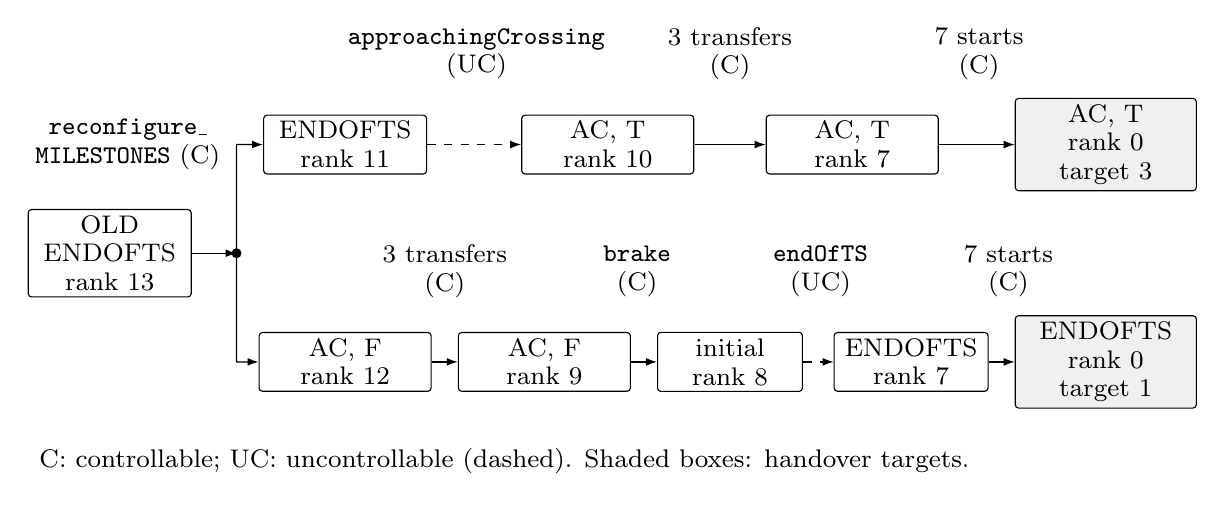
\begin{tikzpicture}[
  x=1mm,y=1mm,scale=1.15,transform shape,
  font=\fontsize{8}{9}\selectfont,
  statebox/.style={draw,rounded corners=1.2pt,line width=.4pt,
    align=center,inner xsep=1pt,inner ysep=2pt,minimum width=18mm},
  goalbox/.style={statebox,fill=black!6,minimum width=20mm},
  edge/.style={-{Latex[length=1.4mm,width=1mm]},line width=.45pt},
  uc/.style={edge,dashed},
  action/.style={align=center,inner sep=0pt}
]
\node[statebox,minimum width=18mm] (source) at (9,0)
  {OLD\\ENDOFTS\\rank 13};
\coordinate (fork) at (23,0);
\node[action] at (11,12)
  {\texttt{reconfigure\_}\\\texttt{MILESTONES} (C)};
\draw[edge] (source.east) -- (fork);
\fill (fork) circle (.55mm);

% Both outcomes belong to the single controllable transfer above.
\node[statebox] (upperA) at (35,12) {ENDOFTS\\rank 11};
\node[statebox,minimum width=19mm] (upperB) at (64,12) {AC, T\\rank 10};
\node[statebox,minimum width=19mm] (upperC) at (91,12) {AC, T\\rank 7};
\node[goalbox] (upperGoal) at (119,12) {AC, T\\rank 0\\target 3};
\draw[edge] (fork) -- (23,12) -- (upperA.west);
\draw[uc] (upperA.east) -- (upperB.west);
\node[action] at (49.5,22) {\texttt{approachingCrossing}\\(UC)};
\draw[edge] (upperB.east) -- (upperC.west);
\node[action] at (77.5,22) {3 transfers\\(C)};
\draw[edge] (upperC.east) -- (upperGoal.west);
\node[action] at (105,22) {7 starts\\(C)};

\node[statebox,minimum width=19mm] (lowerA) at (35,-12) {AC, F\\rank 12};
\node[statebox,minimum width=19mm] (lowerB) at (57,-12) {AC, F\\rank 9};
\node[statebox,minimum width=16mm] (lowerC) at (77.5,-12) {initial\\rank 8};
\node[statebox,minimum width=17mm] (lowerD) at (97.5,-12) {ENDOFTS\\rank 7};
\node[goalbox] (lowerGoal) at (119,-12) {ENDOFTS\\rank 0\\target 1};
\draw[edge] (fork) -- (23,-12) -- (lowerA.west);
\draw[edge] (lowerA.east) -- (lowerB.west);
\node[action] at (46,-2) {3 transfers\\(C)};
\draw[edge] (lowerB.east) -- (lowerC.west);
\node[action] at (67.25,-2) {\texttt{brake}\\(C)};
\draw[uc] (lowerC.east) -- (lowerD.west);
\node[action] at (87.5,-2) {\texttt{endOfTS}\\(UC)};
\draw[edge] (lowerD.east) -- (lowerGoal.west);
\node[action] at (108.25,-2) {7 starts\\(C)};

\node[anchor=west,align=left,font=\fontsize{8}{9}\selectfont] at (0,-23)
{C: controllable; UC: uncontrollable (dashed). Shaded boxes: handover targets.};
\end{tikzpicture}
\caption{Both outcomes of one Railcab/Base transfer after five old stops and before any new start; Base has no interval monitor. AC is approaching-crossing; T/F records whether that event occurred since \texttt{endOfTS}. Boxes show milestone state and rank; targets identify supplied new-controller states. Only single-path sequences of three transfers or seven starts are contracted. Every branch of this 26-state, 25-edge fragment is retained.}
\Description{A controllable milestone transfer has two outcomes. One waits for approachingCrossing, completes transfers and starts, then hands control to controller state 3. The other transfers, brakes, waits for endOfTS, starts the monitors and hands control to state 1. Ranks decrease on every branch.}
\label{fig:railcab-policy}
\end{figure}


Each contracted transfer block uses \texttt{ANOTHER\_REQUEST}, \texttt{REQUEST\_ATOMIC}, then \texttt{TURNS}. Each start block activates, in order, \texttt{P\_BRAKE\_DURING\_LASTBRAKE}, \path{P_BRAKE_IF_SOMETHING_BAD}, \path{P_CHECK_STATUS_AFTER_APPROACHING_CROSSING}, \path{P_CHECK_STATUS_BEFORE_LAST_EMERGENCY_BRAKE}, \path{P_EBRAKE_DURING_ELASTBRAKE}, \path{P_EBRAKE_IF_SOMETHING_BAD}, and \texttt{P\_NEW\_NOT\_CRASH}. Every internal contracted state has exactly one bucket and one outcome. Extraction verifies all 118 rank decreases and both component/new-monitor matches with the fixed endpoint.

\paragraph{R1: two uncontrollable events.}
R1 exports 44 certificate states, 46 buckets, 46 outcomes, one goal and maximum rank 33. It retains seven UPD monitors throughout all 44 certificate states, including its goal. Their guards become true after any old stop until the associated new start. Together they forbid \texttt{requestEnter}, \texttt{brake}, \texttt{emergencyBrake}, \texttt{idle\_c} and \texttt{checkCrossingStatus} during the relevant intervals; they do not forbid uncontrollables. The returned policy performs its ordinary controllable steps before its first stop. Milestone transfers occur at LB or NR and each has one outcome. R1 has \emph{zero} multi-outcome buckets. Its branch at M30 instead has two distinct uncontrollable labels, \texttt{enterAllowed.0} and \texttt{enterAllowed.1}. For entry O1, all 32 descendant states/32 edges are retained; branches merge before the suffix of five stops, three remaining transfers and seven starts. All $46\times7=322$ interval-monitor steps match the source DFA, and the goal matches the physical tuple and NEW monitors of new controller state 3. These are checks of the particular returned certificate, not a proof that every winning policy has this order.

\paragraph{How interval guards change the stop/brake order.}
The Base and R1 exports share old endpoint entry O1, controller state 1, with identical component and old-monitor states. Their update roots are Base M64 (rank 18) and R1 M28 (rank 27); identifiers are local to each export. Base takes five old stops to M69 (rank 13), then its MILESTONES transfer has two outcomes retained in the saved export and the paths below. On the lower branch, three further transfers reach M16 (rank 9), whose brake edge reaches M0 (rank 8).

The R1 prefix, without any old stop, consists of:
\begin{center}\small
\begin{tabular}{lll}
Source & Event & Target\\\hline
M28 (27) & requestEnter (C) & M30 (26)\\
M30 (26) & enterAllowed.0 (UC) & M31 (20)\\
M31 (20) & lastBrake (UC) & M37 (19)\\
M37 (19) & reconfigure\_MILESTONES (C) & M19 (18)\\
M19 (18) & brake (C) & M1 (17)\\
M1 (17) & endOfTS (UC) & M2 (16)\\
M2 (16) & approachingCrossing (UC) & M13 (15)\\
M13 (15) & stopOldSpec\_P\_BRAKE\_DURING\_LASTBRAKE (C) & M14 (14)
\end{tabular}
\end{center}
Parentheses give ranks. The final four sources each have one successor. All five old monitors remain active until M13. The stop removes one and changes all seven R1 monitor guards from 0 to 1. Four further stops, three transfers and seven starts reach M3 (rank 0).

The separate $enterAllowed.1$ branch completes from the same old entry without brake. This extraction does not establish that braking is necessary for every run. The file \path{railcab_stop_brake_paths.csv} preserves every edge of the selected Base/R1 entry-to-goal paths (18/22 edges) and all alternative outgoing edges from states on those selected paths. The accompanying extraction script checks path membership, ownership, ranks, common entry and saved UPD-monitor transitions without rerunning synthesis. Original campaign measurements remain unchanged.

\clearpage
\subsection{Archived auxiliary campaigns and historical checks}
\label{supp:auxiliary-campaigns}
This section retains older sufficient-condition diagnostics, the auxiliary requirement-boundary fixtures, construction/contract variants, and controlled scaling families. They supplement the current RQs without replacing fixed-budget failures or increasing the main constructed-pair denominator.

\subsubsection{Historical initialization coverage}
\paragraph{Archived H/A/E$'$ sufficient-condition results.}
The table preserves the earlier H/A/E$'$ checks. Its E$'$ column records the syntactic test, which leaves 46 R1 occurrences unverified. Lemma~\ref{lem:r1-entry} establishes their exact E initialization using a different sufficient condition. The old result is retained.

\noindent\textbf{RS sufficient-condition coverage}\par
Counts are requirement occurrences over base/R1/R2; repeated new requirements remain in the denominator. The independent free product includes absorbing ERROR and evolving fluent values after error. A failed sufficient check leaves RS untested and does not establish a reachable contract violation.
\begin{center}\scriptsize\begin{tabular}{@{}lrrrrrrrr@{}}\toprule
Model & New / upd & H checked & H FD & H exact & H untested & A sound$^a$ & E$^{\prime}$ exact$^b$ & A/E$^{\prime}$ unverified\\\midrule
GSM & 3 / 3 & 6 & 0 & 0 & 6 & 3 & 2 & 1\\
Industry & 9 / 9 & 18 & 0 & 0 & 18 & 9 & 6 & 3\\
MetaSocket & 3 / 3 & 6 & 0 & 0 & 6 & 3 & 2 & 1\\
PowerPlant & 9 / 10 & 19 & 0 & 0 & 19 & 9 & 7 & 3\\
PC Arms=1 & 18 / 18 & 36 & 0 & 0 & 36 & 18 & 12 & 6\\
PC Arms=2 & 36 / 36 & 72 & 0 & 0 & 72 & 36 & 24 & 12\\
Railcab & 21 / 18 & 39 & 0 & 0 & 39 & 21 & 11 & 7\\
Surveillance & 21 / 21 & 42 & 0 & 0 & 42 & 21 & 14 & 7\\
Workflow & 18 / 17 & 35 & 0 & 0 & 35 & 18 & 11 & 6\\
\bottomrule\end{tabular}\end{center}
FD means that equal reachable fluent valuations determine the same monitor state, including ERROR. Exact additionally requires compatibility with the actual initializer: NEW uses its non-error lookup; UPD uses a constant monitor state after \texttt{hotSwapIn}. Per-requirement state counts, two conflicting histories, and update-boundary checks are in \path{rs-requirements.csv}.
$^a$All \RSAInclusionNew{} NEW occurrences satisfy RS under A: the checked safe-prefix language condition gives equality when the actual safe-history set is nonempty; with an empty set, inclusion is automatic. Plant-level nonemptiness is not established, so exactness remains conditional. $^b$The archived E$^{\prime}$ column uses the syntactic sufficient condition (Lemma E$^{\prime}$): every referenced fluent is declared and affected only by update labels, which cannot occur before entry; the constant initializer must match the non-error state after one \texttt{hotSwapIn}. Remaining event/plant predicates retain unverified reference-language comparisons. Earlier E diagnostic columns and all H/A results are unchanged. Update labels occur at most once in the new prefix explorations; continuation-language equivalence is checked over all words, a stronger condition.


\subsubsection{Auxiliary requirement-boundary inputs}
The capability campaign contains 14 decisions. Its requirement-boundary comparison follows.
\begin{figure}[!htbp]
\centering
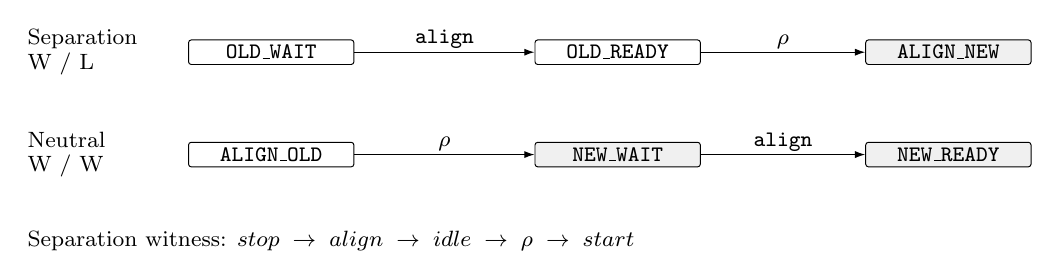
\begin{tikzpicture}[x=1mm,y=1mm,font=\fontsize{8}{9}\selectfont,
  rqnode/.style={draw,rounded corners=1pt,line width=.35pt,inner xsep=2pt,
    inner ysep=2pt,minimum width=21mm,align=center},
  rqedge/.style={-{Latex[length=1.3mm,width=.9mm]},line width=.4pt},
  rqlabel/.style={inner sep=1pt,fill=white}]
\node[anchor=west,align=left,inner sep=0pt] at (0,6) {Separation\\W / L};
\node[anchor=west,align=left,inner sep=0pt] at (0,-7) {Neutral\\W / W};
\node[rqnode] (ow) at (31,6) {\texttt{OLD\_WAIT}};
\node[rqnode] (orr) at (75,6) {\texttt{OLD\_READY}};
\node[rqnode,fill=black!6] (an) at (117,6) {\texttt{ALIGN\_NEW}};
\draw[rqedge] (ow.east) -- node[rqlabel,above] {\texttt{align}} (orr.west);
\draw[rqedge] (orr.east) -- node[rqlabel,above] {$\rho$} (an.west);
\node[rqnode] (ao) at (31,-7) {\texttt{ALIGN\_OLD}};
\node[rqnode,fill=black!6] (nw) at (75,-7) {\texttt{NEW\_WAIT}};
\node[rqnode,fill=black!6] (nr) at (117,-7) {\texttt{NEW\_READY}};
\draw[rqedge] (ao.east) -- node[rqlabel,above] {$\rho$} (nw.west);
\draw[rqedge] (nw.east) -- node[rqlabel,above] {\texttt{align}} (nr.west);
\node[anchor=west,align=left,inner sep=0pt] at (0,-18) {Separation witness: $stop\;\to\;align\;\to\;idle\;\to\;\rho\;\to\;start$};
\end{tikzpicture}
\caption{Measured requirement-boundary inputs. Row outcomes are free/block (W: WIN, L: LOSS). All events are controllable; shaded states are new. Each node has an $idle$ loop; neutral also has $bad$ loops. $\rho$ is the sole transfer. Old/new monitors forbid $align$ in separation and $bad$ in neutral. An interval monitor permits $start$ only after $align$ since entry. A requirement block forbids intervening events/transfers between $stop$ and $start$. Separation is WIN with free boundaries and LOSS with a block; neutral is WIN in both.}
\Description{Separation has an old alignment action before transfer; neutral moves alignment into the new component. Interval constraints require alignment before activating the new monitor.}
\label{fig:rq2-boundary}
\end{figure}

Each input has one old entry. Separation's endpoints allow only $idle$; neutral's old endpoint allows $idle$, and its new controller allows $idle$ and the displayed $align$. OLD/NEW testers have one safe state and an error sink; NEW activation requires a false forbidden-event observer. Entry sets $Aligned$ false. In separation, $align$ sets persistent $Aligned$ and a separate observer of the last ordinary event. $idle$ clears only the observer; update events preserve both.

The source-derived sequence $stop,align,idle,\rho,start$ matches the saved six-state certificate and maximum rank five. Old requirement prevents $align$ before $stop$, so a contiguous block cannot complete. Neutral permits $\rho,align$ before the block. Its block/free runs return ranks four/five; ranks need not be minimal. These are source-derived witnesses and saved certificate counts, not recovered execution traces.

\subsubsection{Granularity and construction ablations}
\label{supp:vthree-ablations}
The E1 transformations are described with the granularity evidence above. The remaining E4/E5 variants and E2 construction comparison are additional campaigns; the generated tables also preserve the full E1 and E6 series indices without expanding the main comparison populations.

E4-1 checks the transformations against saved finite fixtures. Transfer/both merging recovers the cell's losing bulk case. Merging the stop commands with each other and the start commands with each other does not forbid ordinary steps between stop and start: the transformed boundary fixture is therefore distinct from the hand-written contiguous-block restriction. E4-2's corrected Cell$_n$ rings preserve one circulating workpiece; local and boundary-merged inputs win, transfer/both-merged inputs lose. The original series' input-validation errors are retained, not treated as synthesis losses. The series are stored in \path{experiments/witness_20260929/e4_1/} and \path{experiments/witness_20260929/e4_2_corrected/}.

E5 uniformly restricts each physical transfer domain to the declared initial local state. Of \VThreeEFivePairs{} fine/merged pairs, \VThreeEFiveWitness{} separate, \VThreeEFiveBothLoss{} lose both ways, \VThreeEFiveBothWin{} win both ways and \VThreeEFiveIncomplete{} remain unresolved. The \VThreeEFiveTrials{} attempted jobs and \VThreeEFiveNotRun{} deadline-excluded jobs remain separate. Railcab/Base's fine job timed out; its merged job and the other deadline-excluded jobs were not run. Enabled UC requests at the restricted states can prevent a safe quiescent transfer opportunity. Sources and domain checks are in \path{experiments/witness_20260929/e5/tables/}.

E2 changes graph construction alone: Full+UC omits controllable buckets at states with enabled UC events, then constructs the reachable graph before solving. The Mac series has an initial capped pass and a longer pass over its timeouts; its final decisions are \VThreeETwoMacWin{} WIN, \VThreeETwoMacLoss{} LOSS and \VThreeETwoMacTO{} unresolved. State counts, unlike runtime, can be compared across these saved deterministic constructions. On comparable cells, Full+UC is smaller than Direct-Full in \VThreeETwoStateSmaller{} and equal in \VThreeETwoStateEqual{}. It is equal in count to Eager in \VThreeETwoEagerStateEqual{} and larger in \VThreeETwoEagerStateMore{} (GSM/R1 and PowerPlant/R1); equality of the state sets was not checked. OTF without UC pruning is not implemented, so this is an incomplete two-factor comparison. The separate Xeon series uses one fresh trial per cell; Industry/R1 is TO there despite Mac's LOSS. No Mac runtime is used in the paired Xeon table. Sources: \path{experiments/ablation_20260928/tables/} and \path{experiments/ablation_20260928/raw/e2_xeon/}.

\begin{table}[!htbp]
\caption{Construction choices: saved state counts (E2: Mac; other methods: fixed-budget Xeon) and separate Xeon timings. DF = Direct-Full; F+UC = full construction with UC pruning. Time is solve plus internal checking (seconds); F+UC is one trial, Eager a five-run median.}
\label{tab:e2-choices}
\centering\small
\begin{tabular}{@{}lrrrrrr@{}}\toprule
 & \multicolumn{4}{c}{Discovered states} & \multicolumn{2}{c}{Xeon seconds}\\
Input & Lazy & Eager & DF & F+UC & F+UC & Eager\\\midrule
Industry/Base & \VThreeETwoIndustryBaseStatesLazy{} & \VThreeETwoIndustryBaseStatesEager{} & \VThreeETwoIndustryBaseStatesDF{} & \VThreeETwoIndustryBaseStatesFullUC{} & \VThreeETwoIndustryBaseXeonFullUCSec{} & \VThreeETwoIndustryBaseXeonEagerMedianSec{}\\
PC1/Base & \VThreeETwoPCOneBaseStatesLazy{} & \VThreeETwoPCOneBaseStatesEager{} & \VThreeETwoPCOneBaseStatesDF{} & \VThreeETwoPCOneBaseStatesFullUC{} & \VThreeETwoPCOneBaseXeonFullUCSec{} & \VThreeETwoPCOneBaseXeonEagerMedianSec{}\\
PC1/R2 & \VThreeETwoPCOneRTwoStatesLazy{} & \VThreeETwoPCOneRTwoStatesEager{} & \VThreeETwoPCOneRTwoStatesDF{} & \VThreeETwoPCOneRTwoStatesFullUC{} & \VThreeETwoPCOneRTwoXeonFullUCSec{} & \VThreeETwoPCOneRTwoXeonEagerMedianSec{}\\
Railcab/R2 & \VThreeETwoRailcabRTwoStatesLazy{} & \VThreeETwoRailcabRTwoStatesEager{} & \VThreeETwoRailcabRTwoStatesDF{} & \VThreeETwoRailcabRTwoStatesFullUC{} & \VThreeETwoRailcabRTwoXeonFullUCSec{} & \VThreeETwoRailcabRTwoXeonEagerMedianSec{}\\\bottomrule
\end{tabular}
\end{table}

% Generated by paper/scripts/integrate_base_v3_evidence.py from saved evidence only.
\begin{table}[p]
\centering\small
\caption{Selected E2 Xeon timing observations (seconds).}
\label{tab:vthree-e2-timing}
\setlength{\tabcolsep}{3pt}
\begin{tabular}{lrrrr}
\toprule
Contract & Full+UC states & Full+UC (1) & Eager (5 med.) & Ratio \\
\midrule
Industry/Base & 109,726 & 50.455 & 14.516 & 3.48 \\
PC1/Base & 407,019 & 158.667 & 26.016 & 6.10 \\
PC1/R2 & 158,218 & 77.342 & 12.155 & 6.36 \\
Railcab/R2 & 299,700 & 268.563 & 38.669 & 6.95 \\
\bottomrule
\end{tabular}
\par\smallskip\footnotesize Full+UC is one trial; Eager is the median of five valid completed trials. Both timing columns are Xeon observations using the LTS solve-plus-internal-check timer, 64\,GiB heap and 1,200\,s whole-JVM cap. The displayed Full+UC state counts are identical in the saved Mac and Xeon trials. The full E2 structural comparison uses Mac Full+UC counts and existing Xeon counts for the other methods, retaining each marked budget; it pools no times across hosts. Ratios are descriptive, without repetition-based uncertainty for Full+UC. Equal counts do not establish equal state sets. OTF without UC pruning remains unimplemented.
\end{table}

\begin{table}[p]
\centering\small
\caption{Granularity checks on adapted contracts and controlled variants.}
\label{tab:vthree-granularity}
\setlength{\tabcolsep}{3pt}
\begin{tabular}{lrrrr}
\toprule
Series & Comparisons/trials & WIN & LOSS & TO/NR \\
\midrule
E1 transformations & 54 & 51 & 3 & 0 \\
E4 fixtures & 24 & 19 & 5 & 0 \\
E4 corrected rings & 45 & 27 & 18 & 0 \\
E5 scheduled trials & 54 & 4 & 12 & 9/29 \\
\bottomrule
\end{tabular}
\par\smallskip\footnotesize E1 changes no decision in 54 comparisons; 44 discovered-state counts decrease and 10 are equal. The 22 original physical transfer relations are total, which alone does not prove safety or completion. E4 rings cover $n=2,\ldots,10$; the initial series with 30 input errors is retained separately. Boundary batching is not the handmade contiguous-block restriction. E5 has 18 pairs: no witness, six both-LOSS, two both-WIN, ten unresolved; NR denotes the deadline exclusion.
\end{table}

\begin{table}[p]
\centering\small
\caption{E6 registered trials by saved series, with hosts and additional budgets kept separate.}
\label{tab:vthree-e6-series}
\setlength{\tabcolsep}{3pt}
\begin{tabular}{lrrrr}
\toprule
Series & Trials & WIN & LOSS & TO \\
\midrule
rolling/v1 & 100 & 50 & 50 & 0 \\
canary/v1 & 60 & 30 & 30 & 0 \\
policy/v2 & 6 & 3 & 3 & 0 \\
db\_rolling/v2 & 8 & 2 & 6 & 0 \\
rolling\_audit/v1 & 8 & 4 & 4 & 0 \\
threads/v1 & 80 & 40 & 40 & 0 \\
rolling\_scale/v1 & 80 & 40 & 40 & 0 \\
canary\_controls/v1 & 48 & 24 & 24 & 0 \\
pc2\_rolling/v2 & 3 & 1 & 0 & 2 \\
pc2\_rolling/extended\_7200 & 2 & 0 & 0 & 2 \\
pc2\_rolling/xeon\_20260929\_2344 & 3 & 1 & 0 & 2 \\
\bottomrule
\end{tabular}
\par\smallskip\footnotesize The 55 main comparisons are 33 witnesses, 11 both-LOSS, 10 both-WIN and one unresolved PC2 comparison. Rolling scale (20 pairs), Canary controls (12 pairs), and E4 references (9 pairs) are separate. These deliberately constructed cases do not estimate prevalence. PC2 measured TO remains TO despite its separately checked safety obstruction. Audit boundary merging remains WIN; Threads supplies ten both-WIN and ten both-LOSS controls. All new timings are single trials, not medians.
\end{table}


\clearpage
\subsubsection{Controlled families, Travel, and hub scaling}
These are additional scaling populations for current RQ3; RQ4 in generated captions is the archived campaign name. Their first-trial structure, completion eligibility, censored outcomes, and complete plotted ranges are retained below.

\begingroup
% Keep the first generated panel with its introductory heading.
\let\FGClearPage\clearpage
\def\clearpage{\let\clearpage\FGClearPage}
\IfFileExists{build/generated/rq4-controlled.tex}{\clearpage\noindent\textbf{Controlled families: first-trial structure}\par
All 132 jobs are retained. These single trials provide no timing medians.
\begin{longtable}{@{}lrrrr@{}}
\toprule
Model & Lazy & Eager & Update-first & Direct-Full\\\midrule\endhead
ctrl\_fanout\_01 & W: 2 & W: 2 & W: 2 & W: 2\\
ctrl\_fanout\_02 & W: 2 & W: 2 & W: 2 & W: 2\\
ctrl\_fanout\_04 & W: 2 & W: 2 & W: 2 & W: 2\\
ctrl\_fanout\_08 & W: 2 & W: 2 & W: 2 & W: 2\\
ctrl\_fanout\_16 & W: 2 & W: 2 & W: 2 & W: 2\\
transfer\_outcomes\_01 & W: 2 & W: 2 & W: 2 & W: 2\\
transfer\_outcomes\_02 & W: 3 & W: 3 & W: 3 & W: 3\\
transfer\_outcomes\_04 & W: 5 & W: 5 & W: 5 & W: 5\\
transfer\_outcomes\_08 & W: 9 & W: 9 & W: 9 & W: 9\\
transfer\_outcomes\_16 & W: 17 & W: 17 & W: 17 & W: 17\\
uc\_events\_00 & W: 2 & W: 2 & W: 2 & W: 2\\
uc\_events\_01 & W: 3 & W: 3 & W: 3 & W: 3\\
uc\_events\_02 & W: 5 & W: 5 & W: 5 & W: 5\\
uc\_events\_04 & W: 9 & W: 9 & W: 9 & W: 9\\
uc\_events\_08 & W: 17 & W: 17 & W: 17 & W: 17\\
uc\_outcomes\_01 & W: 3 & W: 3 & W: 3 & W: 3\\
uc\_outcomes\_02 & W: 5 & W: 5 & W: 5 & W: 5\\
uc\_outcomes\_04 & W: 9 & W: 9 & W: 9 & W: 9\\
uc\_outcomes\_08 & W: 17 & W: 17 & W: 17 & W: 17\\
requirements\_00 & W: 2 & W: 2 & W: 2 & W: 2\\
requirements\_01 & W: 4 & W: 10 & W: 4 & W: 15\\
requirements\_02 & W: 6 & W: 26 & W: 6 & W: 94\\
requirements\_04 & W: 10 & W: 82 & W: 10 & W: 2556\\
requirements\_08 & W: 18 & W: 290 & W: 18 & W: 1179640\\
precedence\_closure\_00 & W: 5 & W: 11 & W: 5 & W: 16\\
precedence\_closure\_01 & W: 5 & W: 8 & W: 5 & W: 12\\
precedence\_closure\_02 & W: 5 & W: 7 & W: 5 & W: 9\\
precedence\_closure\_03 & W: 5 & W: 6 & W: 5 & W: 8\\
precedence\_closure\_06 & W: 5 & W: 5 & W: 5 & W: 5\\
decision\_transfer\_complete & W: 3 & W: 3 & W: 3 & W: 3\\
decision\_transfer\_partial & L: 3 & L: 3 & L: 3 & L: 3\\
decision\_self\_loop\_controllable & W: 2 & W: 2 & W: 2 & W: 2\\
decision\_self\_loop\_uncontrollable & L: 1 & L: 1 & L: 1 & L: 1\\
\bottomrule\end{longtable}
Cells show decision and discovered states. Queries and outcomes: \texttt{rq4-controlled.csv}.
}{}
\endgroup
\IfFileExists{build/generated/rq4-returned.tex}{\clearpage\noindent\textbf{Travel and hub: completed returns}\par
Travel retains all 48 instances; hub retains 30 seeds under each of three UC profiles.
W/TO/OOM are first-trial counts. Five-run timing eligibility is shown separately.
\begin{center}\small\begin{tabular}{@{}llrrrr@{}}\toprule
Family & Method & W & TO & OOM & Five-run cells\\\midrule
Travel & Lazy & 20 & 26 & 2 & 20\\
Travel & Eager & 20 & 26 & 2 & 20\\
Travel & Update-first & 20 & 26 & 2 & 20\\
Travel & Direct-Full & 18 & 28 & 2 & 18\\
Hub & Lazy & 90 & 0 & 0 & 90\\
Hub & Eager & 90 & 0 & 0 & 90\\
Hub & Update-first & 90 & 0 & 0 & 90\\
Hub & Direct-Full & 90 & 0 & 0 & 90\\
\bottomrule\end{tabular}\end{center}
All completed decisions agree. Travel has 960 planned repetition slots: 504 executed trials and 456 explicit resource-failure skips; hub completes all 1,800 trials.
\texttt{rq4-points.csv} retains all plotted method/instance cells; the two \texttt{rq4-*-comparisons.csv} files retain paired ratios and unresolved statuses.
Travel lazy/Direct-Full state ratios range from 0.03435 to 0.46154 over 18 completed pairs. The upper endpoint is $N=1,K=1$ (12/26 states); all eight $N=1$ ratios exceed one third. No case is excluded to tighten this range.
Lazy and update-first match states, queries and outcomes on all 20 completed Travel instances. Unresolved instances have no measured structure and do not count as equal pairs.
Hub timings are solve-only; Travel LTS timings include the internal checks. Ratios are paired within each family, never pooled across these scopes.
}{}

\begin{table}[!htbp]
\centering\small
\caption{All Travel first-trial outcomes. Entries are Lazy/Eager/Update-first/Direct-Full; W = WIN, T = timeout, O = out of memory.}
\begin{tabular}{@{}lcccccccc@{}}\toprule
$N\backslash K$ & 1 & 2 & 4 & 6 & 8 & 12 & 16 & 20\\\midrule
1 & WWWW & WWWW & WWWW & WWWW & WWWW & WWWW & WWWW & WWWW\\
2 & WWWW & WWWW & WWWW & WWWW & WWWW & WWWW & WWWW & WWWW\\
4 & WWWW & WWWW & WWWT & WWWT & TTTT & TTTT & TTTT & TTTT\\
6 & TTTT & TTTT & OOOO & OOOO & TTTT & TTTT & TTTT & TTTT\\
8 & TTTT & TTTT & TTTT & TTTT & TTTT & TTTT & TTTT & TTTT\\
12 & TTTT & TTTT & TTTT & TTTT & TTTT & TTTT & TTTT & TTTT\\
\bottomrule\end{tabular}
\par\smallskip{\footnotesize $N$ counts amenities; $K$ changes UC choices, path length and local state count together. Each outcome comes from the retained first trial under 1,200 s/64 GiB. Resource failures have no median.}

\end{table}

\begin{figure}[p]
\centering
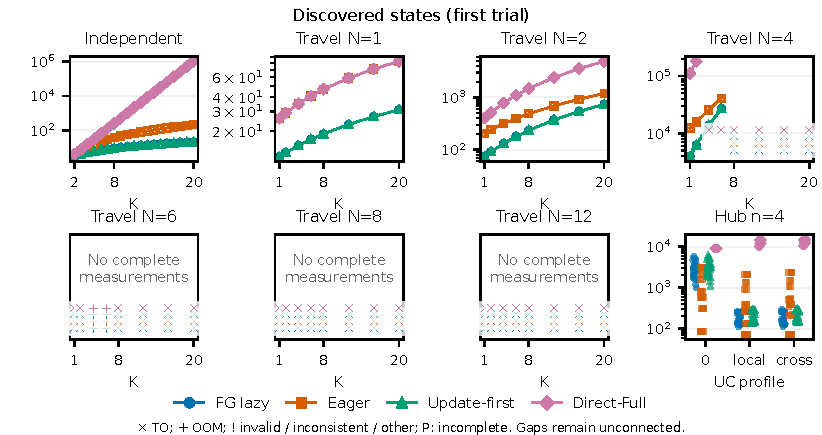
\includegraphics[width=\linewidth]{build/generated/rq4-states-vs-k-full.pdf}
\caption{Full scaling-state panels, retaining every tested Travel concurrency level and every hub profile. RQ4 is the archived campaign name; these results appear under RQ3 (Scaling limits) in the main paper. The saved plots label the independent component count as $K$; it is $n$ in the main paper and S2, distinct from Travel's choice count $K$. Censored outcomes have status marks and no numeric ordinate.}
\end{figure}
\begin{figure}[p]
\centering
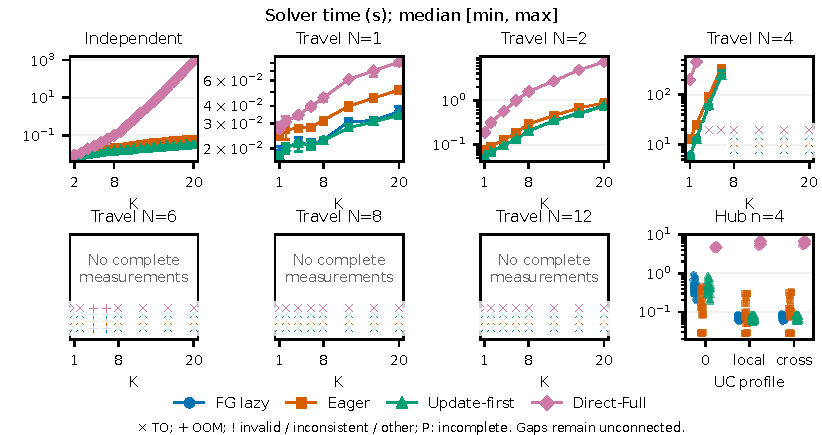
\includegraphics[width=\linewidth]{build/generated/rq4-time-vs-k-full.pdf}
\caption{Full scaling-time panels from the archived RQ4 campaign. Medians and ranges require five valid, consistent completions; TO/OOM and other incomplete outcomes remain visible.}
\end{figure}

\clearpage
\subsection{Extended-budget trials}
\label{supp:extended-budget}
These single trials extend the budget for previously unresolved conditions; the fixed-budget results remain unchanged. Missing raw is not a failed trial, and a capped single trial supplies no five-run median.
% Generated from extended-budget configs and returned evidence.
\providecommand{\ExtBudgetPlanned}{27}
\providecommand{\ExtBudgetChecked}{8}
\providecommand{\ExtBudgetTimeout}{16}
\providecommand{\ExtBudgetOOM}{1}
\providecommand{\ExtBudgetSkipped}{2}
\providecommand{\ExtBudgetPending}{0}
\providecommand{\ExtBudgetReceived}{27}
\providecommand{\ExtBudgetTimeCap}{7{,}200}
\providecommand{\ExtBudgetInitialHeap}{64}
\providecommand{\ExtBudgetExpandedHeap}{200}
\providecommand{\ExtBudgetWins}{7}
\providecommand{\ExtBudgetLosses}{1}
\providecommand{\ExtTravelFourFourDFSeconds}{1{,}872}
\providecommand{\ExtTravelFourFourDFSolverSeconds}{1{,}814}
\providecommand{\ExtTravelFourFourDFStates}{412{,}688}
\providecommand{\ExtTravelFourFourDFRSS}{7}
\providecommand{\ExtTravelFourSixDFSeconds}{6{,}990}
\providecommand{\ExtTravelFourSixDFSolverSeconds}{6{,}768}
\providecommand{\ExtTravelFourSixDFStates}{817{,}362}
\providecommand{\ExtTravelFourSixDFRSS}{13}
\providecommand{\ExtTravelFourEightLazySeconds}{1{,}636}
\providecommand{\ExtTravelFourEightLazySolverSeconds}{756}
\providecommand{\ExtTravelFourEightLazyStates}{47{,}829}
\providecommand{\ExtTravelFourEightLazyRSS}{16}
\providecommand{\ExtTravelFourEightUpdateFirstSeconds}{1{,}655}
\providecommand{\ExtTravelFourEightUpdateFirstSolverSeconds}{718}
\providecommand{\ExtTravelFourEightUpdateFirstStates}{47{,}829}
\providecommand{\ExtTravelFourEightUpdateFirstRSS}{19}
\providecommand{\ExtTravelFourEightEagerSeconds}{2{,}036}
\providecommand{\ExtTravelFourEightEagerSolverSeconds}{961}
\providecommand{\ExtTravelFourEightEagerStates}{64{,}248}
\providecommand{\ExtTravelFourEightEagerRSS}{17}
\providecommand{\ExtIndustryDFSeconds}{1{,}695}
\providecommand{\ExtIndustryDFSolverSeconds}{1{,}693}
\providecommand{\ExtIndustryDFStates}{110{,}825}
\providecommand{\ExtIndustryDFRSS}{3}
\providecommand{\ExtPCOneDFSeconds}{2{,}220}
\providecommand{\ExtPCOneDFSolverSeconds}{2{,}216}
\providecommand{\ExtPCOneDFStates}{3{,}252{,}233}
\providecommand{\ExtPCOneDFRSS}{25}
\providecommand{\ExtWorkflowDFSeconds}{1{,}387}
\providecommand{\ExtWorkflowDFSolverSeconds}{1{,}378}
\providecommand{\ExtWorkflowDFStates}{1{,}774{,}711}
\providecommand{\ExtWorkflowDFRSS}{24}
\providecommand{\ExtSurveillanceDFOOMSeconds}{5{,}271}
\providecommand{\ExtSurveillanceDFOOMSolverSeconds}{--}
\providecommand{\ExtSurveillanceDFOOMStates}{--}
\providecommand{\ExtSurveillanceDFOOMRSS}{211}
\providecommand{\ExtPCTwoLazySeconds}{7{,}205}
\providecommand{\ExtPCTwoLazySolverSeconds}{--}
\providecommand{\ExtPCTwoLazyStates}{--}
\providecommand{\ExtPCTwoLazyRSS}{187}
\providecommand{\ExtTravelSixOneLazySeconds}{7{,}205}
\providecommand{\ExtTravelSixOneLazySolverSeconds}{--}
\providecommand{\ExtTravelSixOneLazyStates}{--}
\providecommand{\ExtTravelSixOneLazyRSS}{79}
\providecommand{\ExtTravelSixOneDFSeconds}{7{,}205}
\providecommand{\ExtTravelSixOneDFSolverSeconds}{--}
\providecommand{\ExtTravelSixOneDFStates}{--}
\providecommand{\ExtTravelSixOneDFRSS}{79}
\providecommand{\ExtFixedMatches}{5}
\providecommand{\ExtFixedComparable}{5}
\providecommand{\ExtFixedUncompared}{3}
\providecommand{\ExtDFHeapFailures}{10}
\providecommand{\ExtDFHeapTimeouts}{9}
\providecommand{\ExtDFHeapTimeoutRSSMin}{159}
\providecommand{\ExtDFHeapTimeoutRSSMax}{213}
\providecommand{\ExtDFPriorRSSMin}{65}
\providecommand{\ExtDFPriorRSSMax}{69}
\providecommand{\ExtDFBothUnresolved}{10}
\providecommand{\ExtLazyHeapPairs}{9}
\providecommand{\ExtLazyHeapSolverUpper}{37.1}
\providecommand{\ExtLazyHeapRSSUpper}{7.4}

\begingroup\scriptsize\setlength{\tabcolsep}{3pt}
\begin{longtable}{@{}llrrrrrrrr@{}}
\caption{Extended-budget single trials (separate from the fixed-budget campaign).}\label{tab:ext-budget}\\
\toprule Cell / campaign & Method & GiB & Cap (s) & Status & JVM (s) & Solver (s) & RSS (GiB) & States & JVM ratio\\\midrule\endhead
Travel(4,4)/base [ext1] & DF & 64 & 7200 & WIN & 1.87e+03 & 1.81e+03 & 7.36 & 412688 & 15.7\\
Travel(4,6)/base [ext1] & DF & 64 & 7200 & WIN & 6.99e+03 & 6.77e+03 & 12.7 & 817362 & 13.4\\
Travel(4,8)/base [ext1] & Lazy & 64 & 7200 & WIN & 1.64e+03 & 756 & 15.9 & 47829 & --\\
Travel(4,8)/base [ext1] & Update-first & 64 & 7200 & WIN & 1.66e+03 & 718 & 19.2 & 47829 & --\\
Industry/r1 [ext2] & DF & 64 & 7200 & LOSS & 1.7e+03 & 1.69e+03 & 2.79 & 110825 & 3.01\\
PC1/r1 [ext2] & DF & 64 & 7200 & WIN & 2.22e+03 & 2.22e+03 & 25.1 & 3252233 & 1.68e+03\\
Travel(4,8)/base [ext3] & DF & 64 & 7200 & TO & 7.2e+03 & -- & 17.2 & -- & --\\
Travel(4,8)/base [ext3] & Eager & 64 & 7200 & WIN & 2.04e+03 & 961 & 17.2 & 64248 & --\\
Travel(4,12)/base [ext3] & Lazy & 64 & 7200 & TO & 7.2e+03 & -- & 32 & -- & --\\
Travel(6,1)/base [ext3] & Lazy & 64 & 7200 & TO & 7.2e+03 & -- & 47 & -- & --\\
Travel(6,1)/base [ext3] & DF & 64 & 7200 & TO & 7.2e+03 & -- & 48.6 & -- & --\\
Railcab/base [ext4] & DF & 200 & 7200 & TO & 7.21e+03 & -- & 190 & -- & --\\
Surveillance/base [ext4] & DF & 200 & 7200 & TO & 7.21e+03 & -- & 213 & -- & --\\
Workflow/base [ext4] & DF & 200 & 7200 & TO & 7.21e+03 & -- & 191 & -- & --\\
Workflow/r1 [ext4] & DF & 200 & 7200 & TO & 7.21e+03 & -- & 192 & -- & --\\
Railcab/r1 [ext4] & DF & 200 & 7200 & TO & 7.21e+03 & -- & 212 & -- & --\\
PC2/base [ext4] & DF & 200 & 7200 & TO & 7.21e+03 & -- & 210 & -- & --\\
PC2/r1 [ext4] & DF & 200 & 7200 & TO & 7.21e+03 & -- & 209 & -- & --\\
Surveillance/r1 [ext4] & DF & 200 & 7200 & OOM & 5.27e+03 & -- & 211 & -- & --\\
Workflow/r2 [ext4] & DF & 200 & 7200 & WIN & 1.39e+03 & 1.38e+03 & 23.6 & 1774711 & 60.1\\
Surveillance/r2 [ext4] & DF & 200 & 7200 & TO & 7.21e+03 & -- & 159 & -- & --\\
PC2/r2 [ext4] & DF & 200 & 7200 & TO & 7.21e+03 & -- & 209 & -- & --\\
PC2/r2 [ext4] & Lazy & 200 & 7200 & TO & 7.21e+03 & -- & 187 & -- & --\\
Travel(6,1)/base [ext5] & Lazy & 200 & 7200 & TO & 7.21e+03 & -- & 78.6 & -- & --\\
Travel(6,1)/base [ext5] & DF & 200 & 7200 & TO & 7.21e+03 & -- & 78.9 & -- & --\\
Travel(6,4)/base [ext5] & Lazy & 200 & 7200 & SKIP & -- & -- & -- & -- & --\\
Travel(6,4)/base [ext5] & DF & 200 & 7200 & SKIP & -- & -- & -- & -- & --\\
\bottomrule\end{longtable}\endgroup
Each row has one planned trial. WIN/LOSS display SUCCESS/UNREALIZABLE; TO is timeout at the stated cap. NOT\_RUN/INCOMPLETE means no completed return; -- means unmeasured or ineligible, never zero. SKIP displays SKIPPED\_MONOTONE, a scheduling exclusion, not a measured resource failure or an inferred losing decision; reasons are in the CSV. ! marks a provenance/check failure; the raw status is retained. The ratio uses total JVM elapsed time divided by the same cell's fixed-budget, five-valid-trial Lazy median (1,200 s, 64 GiB), only for matching checked decisions. It differs from the main paper's solver-time ratios. The CSV separately reports solver-time ratios; timeouts have no ratio. An extended trial is never treated as a five-run median. RSS measures process memory, not heap occupancy.

The \ExtFixedComparable{} comparable extended decisions all match fixed-budget Lazy: Direct-Full on Travel $(4,4)$ and $(4,6)$, Industry/R1 (LOSS), PC1/R1 and Workflow/R2 (WIN). The \ExtFixedUncompared{} Travel $(4,8)$ decisions agree with one another, but fixed-budget Lazy timed out there; they are not baseline decision matches. JVM elapsed time includes preprocessing and other work outside the solver. For Travel $(4,8)$, Lazy, Update-first and Eager have JVM/solver times \ExtTravelFourEightLazySeconds{}/\ExtTravelFourEightLazySolverSeconds{}, \ExtTravelFourEightUpdateFirstSeconds{}/\ExtTravelFourEightUpdateFirstSolverSeconds{} and \ExtTravelFourEightEagerSeconds{}/\ExtTravelFourEightEagerSolverSeconds{} seconds. Table~\ref{tab:ext-budget}'s JVM ratios compare a single extended trial with a fixed-budget Lazy five-run median; the main paper's solver ratios use solver time. Separate solver ratios are retained in the CSV.

Industry/R1's \ExtIndustryDFStates{} states here count the game with goal states terminal. The larger independent-checker count in the Industry/R1 diagnostic above includes reachable states before this truncation, so the enumeration domains differ. Surveillance/R1 has an explicit \texttt{Java heap space} failure. Timeout logs contain no heap-occupancy or GC measurements, so large process RSS alone does not prove a full heap or identify the bottleneck. The \ExtBudgetSkipped{} Travel $(6,4)$ skips record the preregistered unmet success prerequisite for $(6,1)$ under both budgets; they are not observed timeouts or losing decisions.

\paragraph{Additional timeout evidence.}
The generated provenance below retains both the original interrupted attempt and its separate same-setting follow-up. The main PC Arms=2/R2 cell continues to report its original 1,200~s TO; the single 3,600~s result is separate evidence.

\noindent\textbf{Authorized RQ3 follow-ups: original and returned records}\par
Workflow/R2 Direct-Full uses the pre-authorized same-setting replacement for its table status ($\mathrm{TO}^{\ddagger}$). The original operational interruption remains below. PC Arms=2/R2 retains its original 1,200 s TO; the 3,600 s single trial is a separate sensitivity check. Neither follow-up supplies a median or performance ratio.
\begingroup\scriptsize\begin{longtable}{@{}p{.21\linewidth}p{.73\linewidth}@{}}\toprule Field & Recorded value\\\midrule\endhead
Record & PC Arms=2/R2; fg\_ducs\_otf; original\\
Campaign / config & rq3 / config.json\\
Start / end (UTC) & 2026-09-15T09:55:34.006646+00:00 / 2026-09-15T10:15:38.375540+00:00\\
Cap / heap / status & 1200 s / 64g / TIMEOUT\\
Elapsed / peak RSS & 1202.9343 s / 31.2834 GiB (process working set)\\
Original association & rq3/runs/productioncell\_arms2\_\_r2\_\_rep01\_\_fg\_ducs\_otf/meta.json\\
\addlinespace[4pt]
Record & PC Arms=2/R2; fg\_ducs\_otf; supplementary\\
Campaign / config & rq3\_supplement\_pc\_arms2\_r2\_fg\_3600 / config.json\\
Start / end (UTC) & 2026-09-18T06:58:43.395208+00:00 / 2026-09-18T07:58:50.033019+00:00\\
Cap / heap / status & 3600 s / 64g / TIMEOUT\\
Elapsed / peak RSS & 3605.1630 s / 67.1467 GiB (process working set)\\
Original association & rq3/runs/productioncell\_arms2\_\_r2\_\_rep01\_\_fg\_ducs\_otf/meta.json\\
\addlinespace[4pt]
Record & Workflow/R2; direct\_full; original\\
Campaign / config & rq3 / config.json\\
Start / end (UTC) & 2026-09-15T00:12:34.878356+00:00 / not recorded\\
Cap / heap / status & 1200 s / 64g / INTERRUPTED\_NOT\_RETRIED\\
Elapsed / peak RSS & not recorded / not recorded\\
Original association & rq3/runs/workflow\_\_r2\_\_rep01\_\_direct\_full/meta.json\\
\addlinespace[4pt]
Record & Workflow/R2; direct\_full; supplementary\\
Campaign / config & rq3\_supplement\_workflow\_r2\_direct\_full / config.json\\
Start / end (UTC) & 2026-09-18T06:38:27.266316+00:00 / 2026-09-18T06:58:30.415640+00:00\\
Cap / heap / status & 1200 s / 64g / TIMEOUT\\
Elapsed / peak RSS & 1201.6564 s / 13.8951 GiB (process working set)\\
Original association & rq3/runs/workflow\_\_r2\_\_rep01\_\_direct\_full/meta.json\\
\addlinespace[4pt]
\bottomrule\end{longtable}\endgroup
After repetition 1 times out, Workflow repetitions 2--5 have status \path{SKIPPED_AFTER_RESOURCE_FAILURE}; all five planned slots are retained in the generated provenance CSV. The PC follow-up planned one trial.
Returned artifact digests and saved configuration/plan identities are verified. Input bytes, frozen JAR identity, JVM arguments, and stable host/runtime facts match the original records. The PC follow-up changes only the time cap and repetition count. All use the Xeon W-2265, 24 logical CPUs, Windows 10 build 19045, Temurin 17.0.20.1, and a 64 GiB heap cap.
Peak RSS is sampled Windows process working-set memory. Heap occupancy was not recorded; the limiting resource remains unidentified. The recorded elapsed duration includes timeout termination overhead. The interrupted original has no recorded end time or RSS.


\clearpage
% Generated by paper/scripts/integrate_ext7.py.
\subsection{Separate Eager enlarged-heap trials}
\label{supp:vthree-ext-seven}
Each of the \VThreeExtSevenTrials{} conditions has one Eager trial on the same Xeon/JAR as the fixed-budget campaign, with a \VThreeExtSevenHeap{}~GiB Java heap and a \VThreeExtSevenCap{}~s process-time cap; these are single observations, not timing medians, and no Mac times enter this comparison.
All \VThreeExtSevenAgree{} decisions match fixed-budget Lazy; the state ratio is Eager's \texttt{states\_discovered} divided by Lazy's saved \texttt{states\_discovered} (structure repetition~1, equal over all five valid baseline repetitions), and is reported only when both decide.
The \VThreeExtSevenTO{} timeouts and \VThreeExtSevenOOM{} Java-heap OOM have no completed state/query/solver-time record or ratio; their JVM times include termination overhead, and sampled working-set RSS is process memory rather than heap occupancy.
Counts describe the states discovered by the UC-pruned Eager search, which treats unsafe/goal states as terminal; they do not equate its state set with E2 or the unpruned Direct-Full game.

\begin{table}[!htbp]
\centering\footnotesize
\caption{Eager enlarged-heap trials (ext7). W = WIN; L = LOSS; TO = timeout. Times are seconds and RSS is GiB; each timing is one trial.}
\label{tab:vthree-ext-seven}
\setlength{\tabcolsep}{2.5pt}
\begin{tabular}{@{}llrrrrrrrl@{}}\toprule
Condition & Status & States & Queries & Solver & JVM & RSS & Lazy states & Ratio & Src.\\\midrule
Industry/R1 & L & 94,046 & 635,100 & 1,331.5 & 1,333.4 & 2.51 & 38,942 & 2.4 & a \\
Railcab/Base & W & 11,659,723 & 115,706,744 & 2,557.3 & 2,570.3 & 125.54 & 171 & 68,186 & b \\
Workflow/R1 & W & 26,594,216 & 111,677,312 & 2,406.6 & 2,428.9 & 184.94 & 1,098 & 24,221 & c \\
Surv./Base & TO & -- & -- & -- & 7,205.1 & 211.94 & 5,319 & -- & d \\
Railcab/R1 & TO & -- & -- & -- & 7,205.2 & 209.62 & 13,339 & -- & e \\
Surv./R1 & TO & -- & -- & -- & 7,205.1 & 212.13 & 96,301 & -- & f \\
Surv./R2 & W & 10,841,519 & 55,401,437 & 1,575.3 & 1,591.7 & 134.43 & 181,116 & 59.9 & g \\
PC2/Base & TO & -- & -- & -- & 7,205.2 & 209.66 & 2,502 & -- & h \\
PC2/R1 & OOM & -- & -- & -- & 2,981.3 & 209.06 & 2,433 & -- & i \\
PC2/R2 & TO & -- & -- & -- & 7,205.2 & 208.83 & -- & -- & j \\
\bottomrule\end{tabular}
\par\smallskip\raggedright
Solver time includes internal checking; JVM includes preparation and process shutdown.
The status/count/timing fields are cross-checked against each job's \path{meta.json}, \path{output.txt} and \path{stderr.txt}.
Source directories below are relative to \path{experiments/rq3_xeon/raw/ext7_eager_heap200/};
baseline counts come from \path{paper/build/generated/rq3-cells.csv} and agree with all five corresponding raw repetitions.
\par\smallskip
\begin{tabular}{@{}ll@{}}
a & \path{runs/industry__r1__rep01__fg_ducs_otf_eager_controllable/} \\
b & \path{runs/railcab__base__rep01__fg_ducs_otf_eager_controllable/} \\
c & \path{runs/workflow__r1__rep01__fg_ducs_otf_eager_controllable/} \\
d & \path{runs/surveillance__base__rep01__fg_ducs_otf_eager_controllable/} \\
e & \path{runs/railcab__r1__rep01__fg_ducs_otf_eager_controllable/} \\
f & \path{runs/surveillance__r1__rep01__fg_ducs_otf_eager_controllable/} \\
g & \path{runs/surveillance__r2__rep01__fg_ducs_otf_eager_controllable/} \\
h & \path{runs/productioncell_arms2__base__rep01__fg_ducs_otf_eager_controllable/} \\
i & \path{runs/productioncell_arms2__r1__rep01__fg_ducs_otf_eager_controllable/} \\
j & \path{runs/productioncell_arms2__r2__rep01__fg_ducs_otf_eager_controllable/} \\
\end{tabular}\end{table}


\clearpage
\subsection{Legacy reference, archived OTF path and fidelity checks}
\label{supp:legacy-reference}
These original-source/fork comparisons use monolithic conditions and the reference tools' own continued-control objectives. They are decision and fidelity evidence for those contracts, separate from the four same-game FG constructions and from their timing ratios.

\paragraph{Monolithic cross-check: original-source lab build versus this fork.}
The input is the monolithic model from which the fine-grained adaptation was derived. Its bytes match the original-source lab build's bundled model after selecting $T_{\rm Empty}$ instead of $T$; identity with a final published benchmark release remains unconfirmed. Only the two transition-selection lines change. Their definitions remain
\[
\begin{aligned}
T&=(\mathit{StopOldSpec}\land\mathit{TORDone})\Rightarrow
 (\neg\mathit{cancelGF1}\land\neg\mathit{approveGF1}
 \land\neg\mathit{startNewSpec}),\\
T_{\rm Empty}&=(\mathit{StopOldSpec}\land\neg\mathit{StartNewSpec})
 \Rightarrow\neg\mathit{AnyAction}.
\end{aligned}
\]
Both saved logs process the same named old/new safety formulas and $T_{\rm Empty}$, report a 64-state old controller, and use deterministic GR synthesis after safety pruning. They disagree on the update result: the original-source lab build returns a 2,312-state controller, while the fork returns no controller. The fork also reports a 240-state mapping product. Construction counts and the source-level cause appear below. The reference executable is a lab-maintained build of original DUCS source, not an identified official TSE release. Full logs and unchanged input files are in \path{experiments/industry_r1_legacy_monolithic_check/}.

These decision-only results remain separate from RQ3. They rule out interpreting the FG LOSS as general unrealizability of R1: FG requires universal completion from all 131 entries into a compatible verified endpoint at quiescence. Published DUCS synthesizes continued control enforcing the new specification after the switch and takes no fixed new-controller endpoint as input.

\paragraph{Source explanation of the cross-check.}
We compare the fork's synthesis, environment construction and GR-goal code with the
\href{https://git.exactas.uba.ar/lafhis/mtsa/-/tree/d10ba71f092dc9645a80d2752bd089691f158156/maven-root/mtsa/src/main/java/ltsa/updatingControllers}{official MTSA source at commit d10ba71f}.
The inspected official revision is separate from the supplied lab build (source commit e1bf040); the latter JAR is the one used for the recorded GUI result.
Both constructions retain the old closed loop and allow update entry throughout its reachable states; a GR solver's single initial-state check covers that entire pre-update behavior. Both traditional paths synthesize continued control under old/transition/new safety and a GR progress objective. A persistent only-turn-on fluent for the entry event is the GR assumption; persistent stop/start/reconfigure fluents give the three guarantees. Thus the input keyword \texttt{nonblocking} does not make this an existential-only completion check. Neither traditional path checks a fixed new-controller connection or quiescent handover. The supplied fork additionally has a separate OTF branch using \texttt{DirectedController\allowbreak SynthesisDUC} and an endpoint connection map; the inspected official synthesis file at \texttt{d10ba71f} has no such branch. The fork's plain OTF path synthesizes a new controller from the new environment and goal, matches component and new-safety states, and copies the matched controller's transitions into the result. This endpoint connection is therefore not specific to FG-DUCS. It is not used for the Traditional runs here, and inspection of this fork does not establish identity with a historical OTF release.

The upstream formula builder uses the model's \texttt{StopOldSpec}/\texttt{StartNewSpec}. The fork substitutes internal progress fluents (prefix \texttt{\_\_DUC\_}) when reconstructing the violation formulas. Its seven old-safety fluents are TORDone, DSD1Done, Finished, the three validation-event fluents, and internal StopOldSpec. The seven new-safety fluents replace TORDone by NewTORDone and internal StopOldSpec by internal StartNewSpec: their union has nine. \texttt{T\_Empty} adds the model's StopOldSpec/StartNewSpec and eight controllable-event fluents, sharing three validation fluents. Hence the logged total is $9+10-3=16$; these are not 16 additional endpoint obligations.

The fork's update-entry constant is \texttt{hotSwapIn}. The model's two progress fluents still reset on \texttt{beginUpdate}. \texttt{removeTopStates} composes fluent automata even when their labels lie outside the base environment alphabet. Consequently \texttt{beginUpdate} becomes an independent uncontrollable event, resetting the user fluents without resetting the internal ones. With the upstream entry label \texttt{beginUpdate}, that reset instead synchronizes with entry. A finite Python reconstruction of this specific input, without modifying or executing either Java tool, gives:
\begin{center}\small
\begin{tabular}{@{}lrr@{}}
\toprule
Product construction & States & Transitions\\
\midrule
Old controller & 64 & 148\\
Mapping environment & 240 & 1,108\\
Fork entry/reset mismatch & 33,093 & 257,314\\
Synchronized entry/reset & 14,763 & 99,676\\
Fork after safety and at-most-once monitors & 15,177 & 90,250\\
Synchronized after safety and at-most-once monitors & 3,134 & 11,232\\
\bottomrule
\end{tabular}
\end{center}
Both meta-product state/transition pairs exactly match the respective saved logs, as do the 15,177 versus 3,134 final safety-state counts. The synchronized final transition count is reconstructed, not printed by the lab-build log. The mapping count is reconstructed from the supplied model and printed by the fork; the lab-build log does not print that intermediate count. The reconstruction and its assertions are provided as \texttt{check\_legacy\_product.py} beside the two inputs and logs. It checks a concrete encoding discrepancy, not a new result for the frozen 27-instance campaign. The mismatch also explains the fork's negative decision: immediately after \texttt{hotSwapIn}, the safe \texttt{beginUpdate} self-loop can repeat forever without consuming any stop/start/reconfigure event. The GR entry assumption stays true while all three progress guarantees stay false. This uncontrollable trace survives safety and at-most-once filtering. It is a label-compatibility discrepancy, not a new-controller handover requirement. No input, configuration, JAR or synthesis source was changed to obtain this explanation.

The source model's \texttt{AnyAction} includes eight controllable events; its filename and \texttt{T\_Empty} label alone do not establish identity with the published benchmark version.

The fixed RQ3 Legacy reference instead targets \texttt{UPDATE\_CONTROLLER\_FG} and its R1/R2 variants in the nine adapted input files. Those files use \texttt{hotSwapIn} and contain no \texttt{beginUpdate} label. The specific entry/reset mismatch above therefore belongs to the separate monolithic source-input cross-check; this distinction does not establish general source/fork equivalence.

\paragraph{Aligned-entry execution and reference-build identity.}
The reference is a lab-maintained build of original DUCS source at commit \texttt{e1bf040}, with the executable and source identity retained in \path{experiments/legacy_fidelity/}. The eight monolithic inputs agree byte-for-byte across that source revision, compiled resources and executable. This identifies the lab build without asserting an official published-release identity.

A separate fork input changes only the three fluent reset lines for StopOldSpec, StartNewSpec and Reconfigure, replacing \texttt{beginUpdate} by \texttt{hotSwapIn}. One Mac execution of the frozen fork JAR through its Traditional path returns a 2,312-state controller, agreeing with the reference result; the meta-product and final safety input also match at 14,763 and 3,134 states. The earlier mismatched-input failure remains preserved. This is a decision-only fidelity check, excluded from RQ3 and its performance measurements. Input diff, command and original outputs are retained under \path{experiments/legacy_fidelity/}; the returned monolithic reference campaign is reported separately below.

The separate adapter pilot checks Industry under two monolithic conditions (states/transitions below); all four cells return WIN. The aligned fork's $T_{\rm Empty}$ cell reuses that one execution.
\begin{center}\small
\begin{tabular}{@{}lrr@{}}\toprule
Input & Original-source lab build & Aligned fork\\\midrule
Supplied $T$ & 3,050 / 9,496 & 3,050 / 9,496\\
$T_{\rm Empty}$ & 2,312 / 6,615 & 2,312 / 6,615\\\bottomrule
\end{tabular}\end{center}
Two initial adapter failures are preserved: synthesis produced a controller, but an incorrect Java type check rejected the outer composite. Correcting only that adapter yielded the two successful reference-tool cells. The final adapter additionally classifies an explicit no-controller result wrapped in a composition exception; four classification assertions check that branch. These Mac checks supply no performance evidence. The separate Xeon campaign has 21 conditions per tool (15 supplied targets and six named empty-transition alternatives); its returned results remain outside the main RQ3 table.

\paragraph{Returned legacy-fidelity reference experiment.}
These Windows campaigns compare the lab build and fork on mechanically generated monolithic conditions with all three entry-fluent resets aligned. Their contracts differ from FG; the results remain outside RQ3. Table~\ref{tab:legacy-fidelity} retains summaries, per-trial records and fork exceptions. Independently regenerated summaries match the returned CSVs byte-for-byte; raw statuses and reproduction outputs remain in the artifact.

\begingroup\small\setlength{\tabcolsep}{3pt}
\begin{longtable}{@{}p{.29\linewidth}p{.20\linewidth}p{.25\linewidth}p{.20\linewidth}@{}}
\caption{Separate monolithic reference experiment: all 21 conditions. S denotes SUCCESS (controller returned); sizes are first-trial states/transitions. Each completed cell has five consistent SUCCESS decisions; sizes may vary across repetitions (below). N/M labels annotate raw CRASH records, without changing them.}\label{tab:legacy-fidelity}\\
\toprule Input / condition & Original-source lab build & Fork legacy path & Comparison\\\midrule\endfirsthead
\toprule Input / condition & Original-source lab build & Fork legacy path & Comparison\\\midrule\endhead
\bottomrule\endfoot
GSM\newline supplied & S 86/119 & N/M\newline (fork parser) & N/M\\
GSM\newline empty & S 92/117 & N/M\newline (fork parser) & N/M\\
Industry\newline supplied & S 3,050/9,496 & S 3,050/9,496 & MATCH\\
Industry\newline empty & S 2,312/6,615 & S 2,312/6,615 & MATCH\\
MetaSocket\newline UPD64\_128 & S 36/59 & S 36/59 & MATCH\\
MetaSocket\newline UPD64\_64COM & S 36/59 & S 36/59 & MATCH\\
MetaSocket\newline UPD128\_64 & S 36/59 & S 36/59 & MATCH\\
MetaSocket\newline UPD128\_128COM & S 36/59 & S 36/59 & MATCH\\
MetaSocket\newline UPD64COM\_64 & S 36/59 & S 36/59 & MATCH\\
MetaSocket\newline UPD64COM\_128COM & S 36/59 & S 36/59 & MATCH\\
MetaSocket\newline UPD128COM\_128 & S 36/59 & S 36/59 & MATCH\\
MetaSocket\newline UPD128COM\_64COM & S 36/59 & S 36/59 & MATCH\\
PowerPlant\newline supplied & S 79/141 & N/M\newline (fork parser) & N/M\\
ProductionCell\newline supplied & S 168/267 & S 168/267 & MATCH\\
ProductionCell\newline empty & S 107/158 & S 107/158 & MATCH\\
Railcab\newline supplied & S 448/803 & S 443/796 & SIZE-\newline MISMATCH\\
Railcab\newline empty & S 471/708 & S 471/708 & MATCH\\
Surveillance\newline supplied & S 1,394/2,959 & N/M\newline (instrumentation) & N/M\\
Surveillance\newline empty & S 665/1,414 & N/M\newline (instrumentation) & N/M\\
Workflow\newline supplied & S 679/1,144 & S 679/1,144 & MATCH\\
Workflow\newline empty & S 193/287 & S 193/287 & MATCH\\
\end{longtable}\endgroup
The two campaigns retain 210 planned slots: 190 executed trials and 20 explicit skips following the five fork exceptions. Those exceptions occur before a legacy GR decision and give no evidence of legacy synthesis capability or failure.
\paragraph{Saved exception text: fork parser.}
\noindent\texttt{ltsa.lts.LTSException:}\par\noindent\texttt{name already defined\ \ LeavesPumpOn}\par
\noindent\texttt{ltsa.lts.LTSException:}\par\noindent\texttt{name already defined\ \ T\_NO\_UPDATE\_WHILE\_SEND}\par
\paragraph{Saved exception text: instrumentation.}
\noindent\texttt{java.lang.IllegalArgumentException:}\par\noindent\texttt{Derived old-action authority is inconsistent: weather.old}\par
\begin{center}\small
\begin{tabular}{@{}llrrrrr@{}}\toprule
Tool & Condition & Rep. 1 & Rep. 2 & Rep. 3 & Rep. 4 & Rep. 5\\\midrule
Fork & ProductionCell / empty & 107/158 & 102/150 & 107/158 & 102/150 & 107/158\\
Lab build & Railcab / supplied & 448/803 & 448/809 & 449/805 & 443/796 & 442/797\\
Fork & Railcab / supplied & 443/796 & 442/794 & 449/805 & 451/811 & 449/805\\
Lab build & Railcab / empty & 471/708 & 471/708 & 471/708 & 429/651 & 471/708\\
\bottomrule\end{tabular}\end{center}
These are all 4 tool/condition cells whose returned controller sizes vary across the five successful trials; other completed cells retain their first-trial sizes. The fifteen size matches and five-state Railcab difference in Table~\ref{tab:legacy-fidelity} compare first trials only. In particular, the Railcab supplied lab-build trial 4 returns the same size as fork trial 1; a persistent tool-specific size difference or controller equivalence is not established.


\paragraph{Causes of unmeasured fork conditions.}
GSM reuses \path{T_NO_UPDATE_WHILE_SEND} for a property and an assertion; PowerPlant similarly reuses \texttt{LeavesPumpOn}. The original parser checks assertion definitions for name uniqueness, whereas the fork also checks constraints, rejecting these inputs during parsing. This accounts for the three N/M (fork parser) entries, not a synthesis LOSS.

Surveillance declares \texttt{weather} only in \path{NewControllableActions}, not in its old/new alphabets or environment transitions. The fork derives \texttt{weather.old} from the declaration and inserts that derived label into the alphabet. Author-side \path{M9TraditionalSafetySemanticsSnapshot} requires both the derived label and its base action in the alphabet; the absent base \texttt{weather} triggers the saved exception. This capture follows construction of the old controller and meta-environment, but precedes update safety pruning and the legacy GR decision. The two N/M (instrumentation) entries therefore provide no evidence of legacy synthesis capability or failure. No model, tool or JAR was changed and no trial was repeated to repair these outcomes.

\paragraph{Railcab size variation and unresolved cause.}
For supplied Railcab, both logs report 1,763 states before safety pruning and 1,582 afterward, then use nondeterministic controller synthesis. The first-trial difference is already present when the strategy is converted to an MTS and unreachable states are removed, before final CompactState conversion or outer composition. The inspected subset construction, knowledge-game solver and strategy-to-MTS paths share their operative code; preprocessing, fluent-valuation handling and enumeration still differ. The saved evidence does not establish corresponding safety graphs, valuations or strategies. Moreover, controller sizes vary within each tool across repetitions, with some sizes shared across tools. The cause of that variation and the first-trial difference remains unresolved after bounded static inspection; neither a persistent fork effect nor controller equivalence is inferred.

\begingroup\scriptsize\setlength{\tabcolsep}{3pt}
\begin{longtable}{@{}p{.25\linewidth}rrrr@{}}
\caption{Reference measurements only. End-to-end JVM wall seconds and sampled process peak RSS (GiB): median [min,max] only for five complete, consistent runs. No cross-tool ratios are computed.}\label{tab:legacy-fidelity-resources}\\
\toprule Input / condition & Lab wall (s) & Fork wall (s) & Lab RSS (GiB) & Fork RSS (GiB)\\\midrule\endfirsthead
\toprule Input / condition & Lab wall (s) & Fork wall (s) & Lab RSS (GiB) & Fork RSS (GiB)\\\midrule\endhead
\bottomrule\endfoot
GSM\newline supplied & 0.61 [0.609, 0.61] & N/M & 0.102 [0.0995, 0.102] & N/M\\
GSM\newline empty & 0.711 [0.71, 0.712] & N/M & 0.101 [0.0997, 0.105] & N/M\\
Industry\newline supplied & 12.7 [12.6, 12.7] & 16.7 [16.3, 16.8] & 1.91 [1.6, 2.05] & 2.02 [1.97, 2.11]\\
Industry\newline empty & 4.64 [4.44, 4.74] & 7.66 [7.46, 7.77] & 0.814 [0.738, 0.821] & 1.81 [1.73, 1.89]\\
MetaSocket\newline UPD64\_128 & 0.611 [0.609, 0.612] & 1.21 [1.11, 1.21] & 0.0996 [0.0971, 0.103] & 0.14 [0.137, 0.147]\\
MetaSocket\newline UPD64\_64COM & 0.609 [0.608, 0.61] & 1.21 [1.21, 1.22] & 0.0996 [0.0995, 0.0998] & 0.141 [0.139, 0.144]\\
MetaSocket\newline UPD128\_64 & 0.61 [0.609, 0.611] & 1.21 [1.21, 1.21] & 0.0995 [0.0981, 0.0998] & 0.142 [0.14, 0.143]\\
MetaSocket\newline UPD128\_128COM & 0.61 [0.609, 0.61] & 1.21 [1.11, 1.22] & 0.0997 [0.0971, 0.103] & 0.141 [0.14, 0.142]\\
MetaSocket\newline UPD64COM\_64 & 0.61 [0.609, 0.611] & 1.21 [1.11, 1.21] & 0.1 [0.098, 0.103] & 0.144 [0.137, 0.145]\\
MetaSocket\newline UPD64COM\_128COM & 0.609 [0.609, 0.611] & 1.21 [1.21, 1.22] & 0.1 [0.0995, 0.103] & 0.143 [0.139, 0.15]\\
MetaSocket\newline UPD128COM\_128 & 0.61 [0.608, 0.612] & 1.21 [1.11, 1.21] & 0.1 [0.0997, 0.103] & 0.145 [0.141, 0.147]\\
MetaSocket\newline UPD128COM\_64COM & 0.61 [0.608, 0.61] & 1.21 [1.21, 1.22] & 0.102 [0.1, 0.103] & 0.144 [0.141, 0.144]\\
PowerPlant\newline supplied & 0.711 [0.71, 0.712] & N/M & 0.105 [0.101, 0.109] & N/M\\
ProductionCell\newline supplied & 1.11 [1.11, 1.12] & 1.92 [1.92, 1.92] & 0.199 [0.191, 0.206] & 0.303 [0.3, 0.308]\\
ProductionCell\newline empty & 1.12 [1.11, 1.12] & 1.92 [1.82, 1.92] & 0.196 [0.182, 0.204] & 0.309 [0.297, 0.322]\\
Railcab\newline supplied & 1.62 [1.62, 1.72] & 2.63 [2.62, 2.63] & 0.482 [0.472, 0.496] & 0.703 [0.696, 0.711]\\
Railcab\newline empty & 1.82 [1.82, 1.92] & 3.03 [2.93, 3.03] & 0.558 [0.537, 0.566] & 0.682 [0.671, 0.689]\\
Surveillance\newline supplied & 6.35 [5.84, 6.45] & N/M & 0.862 [0.852, 0.867] & N/M\\
Surveillance\newline empty & 10.7 [10.4, 10.8] & N/M & 0.929 [0.877, 0.95] & N/M\\
Workflow\newline supplied & 9.37 [9.17, 9.48] & 12.3 [12.1, 12.4] & 1.03 [0.974, 1.1] & 1.98 [1.96, 2.04]\\
Workflow\newline empty & 4.53 [4.43, 4.64] & 5.65 [5.54, 5.94] & 0.664 [0.631, 0.667] & 1.8 [1.79, 1.94]\\
\end{longtable}\endgroup
Internal times have different scopes: the lab-build adapter includes compilation, continued compilation and composition, whereas the fork exposes its solve-control-problem interval. The table instead uses end-to-end JVM wall time as reference information; these tools do not solve identical FG games and their times are not ratioed. The fork exceptions have one actual trial followed by four explicit skips; no median is reported.

\path{experiments/legacy_fidelity/} holds the inputs, diffs, collector, renderer and raw evidence; the public package omits shaded JARs and the private delta's \texttt{lib/}.

\clearpage
\subsection{Separate Legacy enlarged-heap reference}
\label{supp:vthree-ext-six}
% Generated by paper/scripts/integrate_base_v3_evidence.py from saved evidence only.
% Source: experiments/rq3_xeon/raw/ext6_legacy_heap200/runs/railcab__base__rep01__legacy_ducs/{meta.json,output.txt,stderr.txt}
% Source: experiments/rq3_xeon/raw/ext6_legacy_heap200/runs/workflow__base__rep01__legacy_ducs/{meta.json,output.txt,stderr.txt}
% Source: experiments/rq3_xeon/raw/ext6_legacy_heap200/runs/surveillance__base__rep01__legacy_ducs/{meta.json,output.txt,stderr.txt}
% Source: experiments/rq3_xeon/raw/ext6_legacy_heap200/runs/productioncell_arms2__base__rep01__legacy_ducs/{meta.json,output.txt,stderr.txt}
% Source: experiments/rq3_xeon/raw/ext6_legacy_heap200/runs/railcab__r1__rep01__legacy_ducs/{meta.json,output.txt,stderr.txt}
% Source: experiments/rq3_xeon/raw/ext6_legacy_heap200/runs/workflow__r1__rep01__legacy_ducs/{meta.json,output.txt,stderr.txt}
% Source: experiments/rq3_xeon/raw/ext6_legacy_heap200/runs/surveillance__r1__rep01__legacy_ducs/{meta.json,output.txt,stderr.txt}
% Source: experiments/rq3_xeon/raw/ext6_legacy_heap200/runs/productioncell_arms2__r1__rep01__legacy_ducs/{meta.json,output.txt,stderr.txt}
% Source: experiments/rq3_xeon/raw/ext6_legacy_heap200/runs/railcab__r2__rep01__legacy_ducs/{meta.json,output.txt,stderr.txt}
% Source: experiments/rq3_xeon/raw/ext6_legacy_heap200/runs/workflow__r2__rep01__legacy_ducs/{meta.json,output.txt,stderr.txt}
% Source: experiments/rq3_xeon/raw/ext6_legacy_heap200/runs/surveillance__r2__rep01__legacy_ducs/{meta.json,output.txt,stderr.txt}
% Source: experiments/rq3_xeon/raw/ext6_legacy_heap200/runs/productioncell_arms2__r2__rep01__legacy_ducs/{meta.json,output.txt,stderr.txt}
% Source: experiments/rq3_xeon/raw/ext6_legacy_heap200/runs/productioncell_arms1__r1__rep01__legacy_ducs/{meta.json,output.txt,stderr.txt}
% Source: experiments/rq3_xeon/raw/ext6_legacy_heap200/runs/productioncell_arms1__base__rep01__legacy_ducs/{meta.json,output.txt,stderr.txt}
% Source: experiments/rq3_xeon/raw/ext6_legacy_heap200/runs/productioncell_arms1__r2__rep01__legacy_ducs/{meta.json,output.txt,stderr.txt}
% Source: experiments/rq3_xeon/raw/ext6_legacy_heap200/runs/industry__base__rep01__legacy_ducs/{meta.json,output.txt,stderr.txt}
% Source: experiments/rq3_xeon/raw/ext6_legacy_heap200/runs/industry__r1__rep01__legacy_ducs/{meta.json,output.txt,stderr.txt}
% Source: experiments/rq3_xeon/raw/ext6_legacy_heap200/runs/industry__r2__rep01__legacy_ducs/{meta.json,output.txt,stderr.txt}
\begin{table}[!htbp]
\centering\small
\caption{Separate Legacy extended-budget resource observations: one Xeon trial per condition, 200\,GiB heap and 3,600\,s cap.}
\label{tab:vthree-ext-six}
\setlength{\tabcolsep}{3pt}
\begin{tabular}{llrrrrc}
\toprule
Contract & Display & Peak states & Peak edges & JVM s & RSS GiB & Source \\
\midrule
Railcab/BASE & N/M (profile) & 5,320,658 & 80,379,005 & 1511.9 & 193.94 & a \\
Workflow/BASE & OOM & -- & -- & 3541.4 & 207.59 & b \\
Surveillance/BASE & OOM & -- & -- & 2668.6 & 207.71 & c \\
PC2/BASE & OOM & -- & -- & 1550.6 & 207.80 & d \\
Railcab/R1 & OOM & -- & -- & 3209.7 & 207.71 & e \\
Workflow/R1 & OOM & -- & -- & 3396.3 & 207.64 & f \\
Surveillance/R1 & OOM & -- & -- & 1888.1 & 207.73 & g \\
PC2/R1 & OOM & -- & -- & 1696.5 & 207.75 & h \\
Railcab/R2 & N/M (profile) & 5,320,658 & 80,379,005 & 1646.1 & 200.00 & i \\
Workflow/R2 & OOM & -- & -- & 2593.9 & 207.72 & j \\
Surveillance/R2 & OOM & -- & -- & 2067.3 & 207.79 & k \\
PC2/R2 & OOM & -- & -- & 774.1 & 207.76 & l \\
PC1/R1 & OOM & -- & -- & 2240.0 & 209.41 & m \\
PC1/BASE & N/M (profile) & 1,814,373 & 25,589,560 & 417.2 & 72.76 & n \\
PC1/R2 & N/M (profile) & 1,814,373 & 25,589,560 & 436.2 & 80.83 & o \\
Industry/BASE & N/M (profile) & 683,129 & 8,136,485 & 141.5 & 24.81 & p \\
Industry/R1 & N/M (profile) & 2,888,907 & 34,072,018 & 713.7 & 93.66 & q \\
Industry/R2 & N/M (profile) & 683,129 & 8,136,485 & 145.6 & 25.95 & r \\
\bottomrule
\end{tabular}
\par\smallskip\footnotesize N/M (profile) preserves raw CRASH: all seven records report an IllegalArgumentException at M9MtsSnapshot.requireResourceCensus while capturing the safety meta-environment, before final controller synthesis. The snapshot profile limits include 250,000 states; this is separate from the heap/time budget. State/edge figures are the recorded peak intermediate state space, not a controller or completed solution. All eleven OOM records report Java heap space. RSS is sampled Windows working set, not heap occupancy. Failure runtimes are whole-JVM observations, not successful-solver timings or medians. No decision or general tool limitation is inferred. Text macros round recorded state counts (millions) and OOM RSS (GiB) to one decimal. Sources below are relative to \path{experiments/rq3_xeon/raw/ext6_legacy_heap200/}; each directory supplies meta.json, output.txt and stderr.txt.
\par\smallskip\begin{tabular}{ll}
a & \path{runs/railcab__base__rep01__legacy_ducs/} \\
b & \path{runs/workflow__base__rep01__legacy_ducs/} \\
c & \path{runs/surveillance__base__rep01__legacy_ducs/} \\
d & \path{runs/productioncell_arms2__base__rep01__legacy_ducs/} \\
e & \path{runs/railcab__r1__rep01__legacy_ducs/} \\
f & \path{runs/workflow__r1__rep01__legacy_ducs/} \\
g & \path{runs/surveillance__r1__rep01__legacy_ducs/} \\
h & \path{runs/productioncell_arms2__r1__rep01__legacy_ducs/} \\
i & \path{runs/railcab__r2__rep01__legacy_ducs/} \\
j & \path{runs/workflow__r2__rep01__legacy_ducs/} \\
k & \path{runs/surveillance__r2__rep01__legacy_ducs/} \\
l & \path{runs/productioncell_arms2__r2__rep01__legacy_ducs/} \\
m & \path{runs/productioncell_arms1__r1__rep01__legacy_ducs/} \\
n & \path{runs/productioncell_arms1__base__rep01__legacy_ducs/} \\
o & \path{runs/productioncell_arms1__r2__rep01__legacy_ducs/} \\
p & \path{runs/industry__base__rep01__legacy_ducs/} \\
q & \path{runs/industry__r1__rep01__legacy_ducs/} \\
r & \path{runs/industry__r2__rep01__legacy_ducs/} \\
\end{tabular}
\end{table}


\clearpage
\subsection*{Artifact reproduction status}
The public anonymous repository contains the full derived source tree, saved RQ1/RQ2 evidence, compiled-monitor exports and Python RS checker, and generated tables/figures. The earlier clean HTTPS clone, empty-cache source build and RQ1/RQ2 derive-only smoke checks passed; rederived fields matched the saved expectations after path normalization. Tests were compiled but not executed. Their logs are now under \path{reproduce/previous-validation/clean-clone/}. Third-party dependencies are fetched from official upstream sources; no shaded JAR is distributed. The expanded raw-output package is included in three lossless archive parts within the repository. The current \path{reproduce/check.py} verifies and restores these files, then checks saved correctness/supplement evidence and E-series/ext1--7 results without rerunning benchmarks. The README documents this command and its scope. The implementation and experimental evidence snapshot is identified by tag \texttt{fgducs-invariants-20261002}; the paper-matched PDFs contain the current formal statements and presentation. Its primary reading pair is the main paper and integrated supplementary material, with complete sources and both component PDFs retained for rebuilding and compatibility. The mathematical arguments and presentation use the unchanged experimental observations.

\clearpage
\section{Expanded related-work comparison}
Main-paper Table~2 summarizes three update interfaces. The tables here expand their coverage and progress conditions, then compare synthesis and switching foundations. Publication details appear in the main bibliography. Section and definition numbers identify the inspected native contracts; differences do not establish an inability to encode one approach in another.

\subsection{Update and adaptation interfaces}
\begin{table}[!htbp]
\caption{Native inputs, progress conditions and outputs of update and adaptation approaches.}
\label{tab:supp-native}
\centering\footnotesize
\setlength{\tabcolsep}{3pt}\renewcommand{\arraystretch}{1.05}
\begin{tabular}{@{}>{\raggedright\arraybackslash}p{.15\linewidth}>{\raggedright\arraybackslash}p{.28\linewidth}>{\raggedright\arraybackslash}p{.29\linewidth}>{\raggedright\arraybackslash}p{.23\linewidth}@{}}
\toprule
Work & Inputs and change mechanism & Coverage and progress & Constructed result and scope\\
\midrule
DUCS (2016, 2020)
& One global old-stop/new-start pair, with distinct events; partial, set-valued global $R$; optional stages in $E'$; $T$ constrains order (Secs.~4.2--4.3)
& All old states via total $H$; all outcomes; eventual update events after hotSwap; legal and deadlock-free (Defs.~4.1--4.3)
& Update controller; FLTL control reduction and MTSA synthesis\\
Environment partitioning (2020)
& Pre/post environment LTSs and global state-preservation edges labeled \texttt{reconfigure} ($T_{upd}$)
& The environment construction joins supplied pre/post states; subsequent control uses the existing update-synthesis method
& Generated $E_{upd}$ from $E_{bef}$, $E_{aft}$ and $T_{upd}$ (Sec.~V, Algorithm~1)\\
GR(1) updating (2022)
& Two specifications and switching assertion; old safety guarantees before switch, new specification afterward
& All prefixes meeting new environment safety; uniformly bounded switch (Def.~3.1); subsequent GR(1) liveness assumes justice
& New controller $C_2$ and symbolic reachability bridge; switching bookkeeping; winning set $W$ or current-state early stop (Sec.~4)\\
Live Synthesis (2022)
& Old/new LTL and trace or transition system; residual $\Psi(\eta,\varphi)$; old obligations finitely satisfied
& Universal variant: all old finite traces and new traces; reduction assumes one eventual update (Thm.~6.4)
& Obligation monitor and LTL synthesis; LiveLTL language inclusion\\
Jiao et al. (2013)
& Existing workcell supervisor and added machine; event relabeling and communication transitions produce coordinated supervisors (Sec.~III.B)
& Old states map to new supervisor-state pairs; instant switching is assumed faster than UC events (Sec.~III.C)
& Reuses and transforms the controller; the example checks equivalence to monolithic synthesis; no staged all-outcome handover search\\
Dynamic Feature (2024)
& Feature come/go, component reinitialization, simultaneous changes; behavioral/configuration constraints
& Mixed controllability; UC preserved; every reachable controlled state has a jointly marked continuation (Sec.~7)
& CIF BDD synthesis; maximal safe controllable nonblocking supervisor\\
Zhang et al. (2005)
& Configurations, dependency invariants, adaptive actions, implementations and costs; generated safe adaptation graph (Secs.~3.1, 4.1--4.2)
& Supplied source/target request; minimum-cost path; failed steps may roll back or await intervention (Sec.~4.4)
& Dijkstra path and manager/agent protocol; action-specific safe states, atomic isolated adaptation (Secs.~3.1, 4.3)\\
Network updates (2015)
& Per-switch replacement; searched update order; packet-flush waits
& All single-packet traces satisfy LTL; failure freedom, fair forwarding, bounded processing (Sec.~3.1)
& Sequence; DFS and incremental checking; simple/careful completeness\\
\bottomrule
\end{tabular}
\end{table}

\clearpage
\subsection{Synthesis and supervisory switching}
Existing synthesis and switching methods supply foundations for FG-DUCS. In particular, state correspondence and switching between existing supervisors are established ideas. FG-DUCS combines supplied endpoints with staged component transfers, individual requirement lifetimes and finite completion under all permitted outcomes.
\begin{table}[!htbp]
\caption{Synthesis and switching contracts. An available completing continuation differs from completion of every maximal update run.}
\label{tab:supp-foundations}
\centering\footnotesize
\setlength{\tabcolsep}{3pt}\renewcommand{\arraystretch}{1.05}
\begin{tabular}{@{}>{\raggedright\arraybackslash}p{.15\linewidth}>{\raggedright\arraybackslash}p{.28\linewidth}>{\raggedright\arraybackslash}p{.29\linewidth}>{\raggedright\arraybackslash}p{.23\linewidth}@{}}
\toprule
Work & Inputs and change mechanism & Coverage and progress & Constructed result and scope\\
\midrule
DCS (2016)
& Deterministic component LTSs; safety/co-safety event goals
& Initial product state; safety and eventual goal occurrence on every closed-loop trace; states enabling controllable and UC events treated as UC
& Controller or failure; heuristic OTF composition, deferred control alternatives and backward propagation (Secs.~I, III--IV)\\
OTF-DCS (2023)
& Component automata, marked/illegal states and control partition
& All UC enabled; designated disturbances; eager director (Def.~3); every controlled finite trace has a marked extension (Def.~4)
& Safe nonblocking director; heuristic OTF composition\\
Tripakis--Altisen (1999)
& Finite game graph, controllable/UC edges, safe/target sets
& UC-successor closure; controllable path to target from each node (Sec.~2.1); environment may move first
& Strategy subgraph; fully OTF for untimed graphs\\
Strong planning (1998)
& Action/fluent domain, nondeterministic effects and goal formula
& All initial states and outcomes; strong completion; fair iterative extension separate (pp.~40--43)
& OBDD state/action plan; universal outcome preimages; initial-set early stop\\
DES state attraction (2015)
& Common deterministic plant; request/startup sets; task language $K$ and recognizer
& All request states; UC preserved; weakly invariant startup set; bounded first completion (Def.~2, Thm.~1)
& Attractor supervisor; plant/recognizer product and state-attraction algorithm\\
Switched supervisory control (2020)
& One plant and two safe/live supervisors; switching and state-reinitialization functions (Sec.~3.3, Defs.~4--6)
& Safe, deadlock-free switching; every finite trace has an extension reaching a switching opportunity (Problem~1); repeated switching
& Also synthesizes the supervisor pair; supplied-pair construction retains compatible plant/supervisor states, not a one-time finite completion objective\\
Switched DES invariants (2017)
& Given operational modes and transitions, uncontrollable mode switches and a safety predicate per mode (Sec.~II)
& Invariants under every permitted transition; all mode switches retained; finite convergence concerns computation, not handover time
& Maximally permissive supervisor; distributed modal computation reaches the same solution (Thms.~1--2)\\
\bottomrule
\end{tabular}
\end{table}

\end{document}
